% master.tex : master file for the project
% ------------------------------------------------------------------------------
% This is the main file in the project, which collects the contents from all the
% input files (text, images, literature databases, etc.).

% The 'book' class is a document class with many flexible options.
% See https://tex.stackexchange.com/a/36989/118167
\documentclass[11pt,a4paper,oneside,openright,english]{book}

% Some top level variables that are used to automatically input title, authors,
% etc. in the title page and front page.
\def \projecttitle       {Ramsey Theory}
\def \projectsubtitle    {An Introduction to Graph Ramsey Theory and Partition Regularity over $\mathbb{N}^{+}$}
\def \projecttheme       {Combinatorics\\\-\ Ramsey Theory\\\-\ Graph Theory}
\def \projectdegree      {Mathematics}
\def \projectperiod      {Spring Semester 2024}
\def \projectnumber      {P8}
\def \projectgroup       {1.217c}
\def \projectauthors     {
	Martin Sig Nørbjerg\\
	% ...
}
\def \projectsupervisors {
	Matteo Bonini
	% ...
}

% The preamble, i.e. all the settings and commands that go before actual
% document contents, in this template is handled in the single file aaumath.sty,
% which defines a package that can be loaded here with \usepackage.
\usepackage{aaumath}

% All contents of the document go between the \begin and \end commands for the
% 'document' environment.
\begin{document}

\DeclareTOCStyleEntry[
	beforeskip=.3em plus 0pt,% default is 1em plus 1pt
	pagenumberformat=\textbf
]{tocline}{chapter}
% The front matter is not counted in the numbered pages and are instead numbered
% with roman numerals. This consists of, for exmp, the front page, title
% page, preface, and table of contents.
\frontmatter
% incl/misc/frontpage.tex : document front page
% ------------------------------------------------------------------------------

\newpagecolor{black}
\backgroundsetup{
  scale = 1,
  angle=0,
  opacity=1,
  contents = {
    
\includegraphics[width=\paperwidth,height=\paperheight]{fig/img/aau/waves/AAU_BOELGER_WHITE-10.png}
  }
}
\BgThispage
\pdfbookmark[0]{Front page}{frontpage}
\begin{titlepage}
  \centering
  \phantom{}
  \vspace{2cm}

  % AAU badge
  \begin{minipage}[c]{0.2\paperwidth}
    \centering
    \makebox[0pt]{
      % fig/tikz/aau-badge.tex : AAU logo badge for the front page
% ------------------------------------------------------------------------------

\begin{tikzpicture}
  % Draw white circle and add the transparent blue logo on top
  \node[circle,color=white,fill=black,minimum size=1.175\textwidth] at (0,0) {};
  \node at (0,0) {
\includegraphics[width=\textwidth]{fig/img/aau/logos/AAU_UK_CIRCLE_white_rgb.png}};
\end{tikzpicture}

    }
  \end{minipage}

  % Main contents
  \vspace{4cm}
  {\fontfamily{bch}\selectfont
    \fboxsep0pt
       \colorbox{white}{
          \begin{minipage}{\textwidth}
        \centering
        \color{black}

        \vspace{2em}
        {\Huge\bfseries\projecttitle}

        {\Large\bfseries\projectsubtitle}

        \bigskip
        \parbox{\textwidth}{\centering\large\projectauthors}

        \bigskip
        {\bfseries\large{\projectnumber} Project, Group \projectgroup, \projectdegree}
        \vspace{2em}
      \end{minipage}
    }
  }

\end{titlepage}
\restorepagecolor

% incl/misc/titlepage.tex : project title page
% ------------------------------------------------------------------------------
% The title page is generated by the command \aautitlepage, which is defined in
% /incl/pre/ext/aautitlepage.sty


\pdfbookmark[0]{Title page}{titlepage}
\aautitlepage{
  \projectinfo{
    \projecttitle
  }{
    \projecttheme
  }{
    \projectperiod
  }{
    Group \projectgroup
  }{
    \parbox[t]{\textwidth}{\projectauthors}
  }{
    \parbox[t]{\textwidth}{\projectsupervisors}
  }{
    \today
  }
}{
  \textbf{Dept. of Mathematical Sciences}\\
  Skjernvej 4A\\
  DK-9220 Aalborg Ø\\
  \href{http://math.aau.dk}{http://math.aau.dk}
}{
  % incl/misc/abstract.tex : project abstract
% ------------------------------------------------------------------------------
% The abstract is a short summary of the document, displayed on the title page

}

\chapter*{Preface}

%This is a P8 project written at the Department of Mathematical Sciences at Aalborg University.
%As such the reader is expected to have the general knowledge acquired during a bachelors degree in mathematics at Aalborg University. This project builds on my bachelors thesis \citep{bachellor} on the construction of algebraic geometry codes (AG codes), hence it is expected that the reader is familiar with the following:
%\begin{itemize}
%  \item The basic notions of linear error correcting codes.
%  \item The basics of the theory of projective, regular and absolutely irreducible curves over $\mathbb{F}_q$ and in particular the Riemann-Roch spaces associated with these curves.
%  \item The basic construction and properties of AG codes\footnote{Here we mean evaluation codes (The theory of residue codes will be introduced in Chapter \ref{chap:AG_codes})}, that is codes of the form $\mathcal{C}_L(\mathcal{X}, D, G)$ where $D$ and $G$ are divisors on the curve $\mathcal{X}$ such that the support of $D$ and $G$ is disjoint.
%\end{itemize}

The work on the project took place from the 1. of September to the 20. of December 2023.

Sources are stated at the start of each chapter, or section if the sources used in that particular section differ from the sources, which are generally used within the chapter.

Definitions, algorithms, theorems, propositions, lemmas, corollaries, examples, and remarks are numbered according to each chapter and consecutively.
Equations are also numbered according to each chapter but separately and likewise with figures and tables.
The conclusions of proofs and examples are marked with $\blacksquare$ and $\square$ respectively.

A table of notation and shorthands is given after the list of contents.
Please note that some symbols may be used differently in different chapters.

%Finally, I wish to thank and acknowledge my supervisor Matteo Bonini for his guidance and for being indulgent enough, to answer questions with no imitate application to the project.
Finally, I wish to extend a thank you to my supervisor, Matteo Bonini, for his wonderfull guidance throughout the project.

\vspace{\baselineskip}\hfill Aalborg University, \today
\vfill\noindent

\begin{minipage}[H]{\textwidth}
 \centering
 \rule{\textwidth / 2}{1pt}\\
  Martin Sig Nørbjerg\\
 {\footnotesize mnarbj20@student.aau.dk}
\end{minipage}
\hfill

% incl/misc/contents.tex :
% ------------------------------------------------------------------------------

\pdfbookmark[0]{Contents}{contents}

% The settings in this file are grouped so they only apply here
\begingroup

% Temporarily disable twoside layout to avoid blank pages in this section
\makeatletter
\@twosidefalse
\makeatother

% Put table of contents on its own page (best for a TOC that fits on one page)
\tableofcontents
\clearpage

% Put the lists on subsequent pages without page breaks
%\let\clearpage\relax
%\listoffigures
%\listoftables
%\listofalgorithms
%\lstlistoflistings

\endgroup

\chapter*{Notation and Shorthands}


% The main matter is were the bulk of your work goes. Pages and headings have
% arabic numbers.
\mainmatter

\chapter{Introduction to Ramsey Theory}
%Suppose we have some arbitrary finite coloring $\chi$ on some structure mathematical structure $S$, that is some function $\chi: S \to C$, where $C$ is some set of colors. Given a family of substructures $\mathcal{S}$ of $S$ does $\chi$ admit a monochromatic element in $\mathcal{S}$, provided $S$ is sufficiently large? Ramsey theory is the study of exactly these types of mathematical problems,
Consider some mathematical structure $S$ and a family $\mathcal{F}$ of substructures of $S$. Does every finite coloring $\chi$ on $S$, that is every function $\chi: S \to C$ where $C$ is a finite set of colors, admit a monochromatic element in $\mathcal{F}$, provided $S$ is sufficiently large and if so how large does $S$ have to be? Ramsey theory is the study of exactly these kinds of questions. The theory is quite vast, for instance it includes results on Euclidian geometry and ergrodic theory. So naturally we will focus on the areas of Ramsey theory which are relevant to the field of discrete mathematics. More explicitly we will consider graph Ramsey theory and Ramsey theory over $\mathbb{N}^{+}$, in Chapters \ref{chap:graph_ramsey} and \ref{chap:partition_regularity} respectively.

Chapter \ref{chap:graph_ramsey} starts by establishing Ramsey's theorem, which states that given $\ell_1, \ell_2, \ldots, \ell_{r} \in \mathbb{N}^+$ there exists a least natural number $n = R(\ell_1, \ell_2, \ldots, \ell_{r})$, called a Ramsey number, such that every $r$-coloring $\chi: E(K_n) \to \left\{c_1, c_2, \ldots, c_{r}\right\}$ admits some clique $\mathcal{C}$ of order $\ell_i$ with the edges in $\mathcal{C}$ being colored $c_i$ by $\chi$. In Sections \ref{sec:upper_bound} and \ref{sec:lower_bound} we prove some lower and upper bounds on $R(\ell_1, \ell_2, \ldots, \ell_{r})$. This is followed by Section \ref{sec:exact_values} which establishes the exact values of some small Ramsey numbers. Finally in Section \ref{sec:ass_ramsey} we study the asymptotic behaviors of certain types of Ramsey numbers.

Chapter \ref{chap:partition_regularity} is divided into three main sections each of which dedicated to a distinct theorem from Ramsey theory over $\mathbb{N}^{+}$:
\begin{enumerate}[label=\arabic*.]
	\item The first section covers van der Waerden's Theorem \ref{thm:van_der_waerden}, which asserts that for every $r, k \in \mathbb{N}^+$ there exists a least natural number $W(k, r)$ such that every $r$-coloring of $[1; W(k, r)]$ admits a monochromatic arithmetic progression, that is a set of the form $\left\{a, a + d, \ldots, a + (k- 1)d\right\}$ for some $a, d \in \mathbb{N}^{+}$. Additionally we study a lower bound, constructed using the theory of finite fields, originally proposed by Berlekamp.
	\item The next section covers Schurs Theorem \ref{thm:additive_schur}, which state that there exists a least natural number $S(k, r)$ such that every $r$-coloring of $[1; S(k, r)]$ admits a monochromatic set of the form $\left\{x_1, x_2, \ldots, x_{k}, \sum^k_{i = 1} x_i\right\}$. One of the neat results which follows from Schurs Theorem, is that for each $n \in \mathbb{N}^{+}$ there exists a prime $p$ such that for all primes $q \geq p$, the equation $x^{n} + y^{n} = z^{n}$ has a non-trivial solution in $\mathbb{F}_q$. We conclude this section by studying the asymptotics of $S(2, r)$.
	\item The final section is on Rados Theorems \ref{thm:single_eq_rado} and \ref{thm:rado_full}, we provide a proof of his single equation theorem (Theorem \ref{thm:single_eq_rado}), which classifies which homogeneous linear equations are guarantied\footnote{In the sense that it holds for every finite coloring of $\mathbb{N}^{+}$.}have monochromatic solutions in $\mathbb{N}^+$. From this we are also able to completely characterize which non-homogeneous equations are guarantied to have monochromatic solutions.
\end{enumerate}

\chapter{Graph Ramsey Theory}\label{chap:graph_ramsey}
This chapter introduces graph Ramsey theory, and is based upon \cite{rt} and \cite{rtoi}[Chapter 1]. We will start by introducing the concept of a coloring and some related concepts.
\begin{definition}
	Let $A$ be a set, an \textit{$r$-coloring} on $A$ is a function $\chi: A \to C$ where $C$ is the set of \textit{colors} and $\abs{C} = r$. Let $a \in A$ if $\chi(a) = c$, then $a$ is said to be \textit{colored} $c$ by $\chi$. The subset $B \subseteq A$ is called \textit{monochromatic} if $\abs{\chi(B)} = 1$. Finally if $\mathcal{F} \subseteq \mathcal{P}(A)$ we say that $\chi$ \textit{admits} a monochromatic instance in $\mathcal{F}$ is there exists some monochromatic $B \in \mathcal{F}$.
\end{definition}
In order to visually illustrate the ideas presented through examples we often simply color (this time literally) each object a given color.

\begin{remark}\label{rem:color_sets}
The concrete choice of color set $C$, in our $r$-coloring $\chi: A \to C$, is not really a concern, since given any bijection $\phi$ between $C$ and another color set $C'$ one would obtain a new $r$-coloring $\chi' = \phi \circ \chi$.
Hence for the sake of simplicity we usually pick $C = \left\{c_1, c_2, \ldots, c_{r}\right\}$, unless $r = 2$ or $r = 3$ in which cases we usually let $C = \left\{red, blue\right\}$ or $C = \left\{red, blue, green\right\}$ respectively.
\end{remark}
\begin{remark}\label{rem:correspondence_between_colorings_and_partition}
	Every $r$-coloring $\chi: A \to \left\{c_1, c_2, \ldots, c_{r}\right\}$, corresponds to a partition of $A$ into $r$-subsets, that is the sets $A_{i} = \left\{a \in A \middle| \chi(a) = c_{i}\right\}$ for $i \in [1; r]$, and vice versa. Throughout the project we will use this correspondence, to use what ever framework is deemed most appropriate.
\end{remark}
The following theorem will play a pivotal role, in establishing some of the more elemental results.
\begin{theorem}[Generalized Pigeonhole Principle]\label{thm:gpp}
	Let $m, r \in \mathbb{N}^{+}$ and $A$ be a set such that $\abs{A} \geq m \cdot r$, if $A_1, A_2, \ldots A_r \subseteq A$ such that $A = \bigcup_{i = 1}^{r} A_i$, then there exists an $A_j$ with $\abs{A_j} > m$.
\end{theorem}
\begin{proof}
	Assume for the sake of contradiction that $\abs{A_j} < m$ for all $j = [r]$, then:
	\begin{equation*}
		\abs{A} \leq \sum_{j = 1}^r \abs{A_i} < r \cdot m
	\end{equation*}
	clearly a contradiction.
\end{proof}
We will primarily use the Generalized Pigeonhole Principle (Theorem \ref{thm:gpp}) by using the natural correspondence between partitions and colorings as desribed in Remark \ref{rem:correspondence_between_colorings_and_partition}.

Throughout this section we will primarily be interested in the case where $A$ is the set of edges $E$ of some graph $G$, in which case we will refer to $\chi$ as an \textit{edge coloring} on $G$.
Hence we shall need some basic notions from graph theory. Throughout the rest of this project a graph shall refer to a simple graph, unless otherwise specified. We say that a subgraph $H$ of $G$ is monochromatic, under $\chi$, if every edge in $H$ is colored the same color by $\chi$

\begin{definition}
	Let $G = (V, E)$ be a graph, $G$ is called \textit{complete} if $v, u \in V$ such that $v \neq u$ implies $\left\{v, u\right\} \in E$. A \textit{subgraph} of $G$ is a graph $G' = (V', E')$ such that $V' \subseteq V$ and $E' \subseteq E$. Finally a complete subgraph is called a \textit{clique}.
\end{definition}
\begin{remark}
	Given a graph $G$ we will some times abuse the notation and simply write $V(G)$ to mean the vertex set of $G$ and $E(G)$ to mean the edge set of $G$.
\end{remark}
We often denote a complete graph with $n$ vertices as $K_n^{*}$ or $K_n$. With the conventions that $V(K_n^{*}) = [0; n - 1]$ and $V(K_n) = [1; n]$ that is the sets $\left\{0, 1, \ldots, n - 1\right\}$ and $\left\{1, 2, \ldots, n\right\}$ respectively.

\begin{definition}\label{def:cliques_and_neighbours}
	Let $G = (V, E)$ be a graph and $U \subseteq V$. We denote the subgraph of $G$ consisting of the vertices in $U$ by $G|_U$ that is:
	\begin{equation*}
		G|_U := \left(U, E \cap (U \times U)\right)
	\end{equation*}
	If $\chi: E \to C$ an $r$-edge coloring on $G$, we will define the set:
	\begin{equation*}
		\mathcal{C}_{\chi}(G; \ell) := \left\{ G|_{U} \middle| U \subseteq V, \abs{U}  = \ell \text{ and }  \abs{\chi(E \cap \left(U \times U)\right)} = 1 \right\}
	\end{equation*}
	That is $\mathcal{C}_{\chi}(G; \ell)$ is the set of all monochromatic cliques (under $\chi$) of order $\ell$, note that $\chi$ may be omitted if no confusion is likely to be occur. Additionally we let:
	\begin{equation*}
		\mathcal{N}_{\chi}(v; c) := \left\{u \in V \middle| \{u, v\} \in E \text{ and } \chi\left(\left\{u, v\right\}\right) = c\right\}
	\end{equation*}
	That is $\mathcal{N}_{\chi}(v; c)$ is the set of notes adjacent to $v$ through a $c$-colored edge. Again we may simply write $\mathcal{N}(v; c)$ if no confusion is likely to occur.
\end{definition}
\begin{example}\label{exmp:cliques_and_neighbours}
	To illustrate the contents of Definition \ref{def:cliques_and_neighbours} we will consider graph the $G$ and  $2$-edge coloring, illustrated in figure \ref{fig:cliques_and_neighbours}.
	\begin{figure}[H]
		\centering
		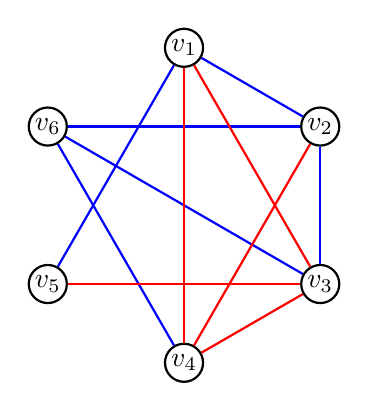
\begin{tikzpicture}
			\tikzset{punkt/.style={circle, thick, draw=black, minimum width=0.2cm,inner sep=1}}
			\node[punkt] at (0.0, 2.0) (a) {$v_1$};
			\node[punkt] at (1.73, 1.0) (b) {$v_2$};
			\node[punkt] at (1.73, -1.0) (c) {$v_3$};
			\node[punkt] at (0.0, -2.0) (d) {$v_4$};
			\node[punkt] at (-1.73, -1.0) (e) {$v_5$};
			\node[punkt] at (-1.73, 1.0) (f) {$v_6$};
			%\draw (0,0) circle [radius=2];

			% Blue edges
			\draw [thick, draw=blue] (a) -- (b);
			\draw [thick, draw=blue] (b) -- (c);
			\draw [thick, draw=blue] (e) -- (a);
			\draw [thick, draw=blue] (f) -- (d);
			\draw [thick, draw=blue] (f) -- (b);
			\draw [thick, draw=blue] (f) -- (c);

			% Red edges
			\draw [thick, draw=red] (a) -- (c);
			\draw [thick, draw=red] (c) -- (d);
			\draw [thick, draw=red] (b) -- (d);
			\draw [thick, draw=red] (c) -- (e);
			\draw [thick, draw=red] (a) -- (d);
		\end{tikzpicture}
		\caption{A graph $G$ with a $2$-edge coloring}
		\label{fig:cliques_and_neighbours}
	\end{figure}
	We see that $\mathcal{C}(G; 3) = \left\{G|_{\{v_1, v_2, v_3\}}, G|_{\{v_2, v_3, v_{6}\}}\right\}$ additionally we see that $\mathcal{N}(v_3; red) = \left\{v_1, v_{4}, v_5\right\}$ and $\mathcal{N}(v_3; blue) = \left\{v_2, v_{6}\right\}$.
\end{example}

\section{Existence of Ramsey Numbers}
This section is based upon \cite{rt}[Section 1.1].
\begin{definition}
	Let $\ell_1, \ell_2, \ldots, \ell_r, n \in \mathbb{N}^{+}$ we will write $n \to (\ell_1, \ell_2, \ldots, \ell_{r})$ if for every $r$-edge coloring $\chi: E(K_{n}) \to \left\{c_1, c_2, \ldots, c_{r}\right\}$ on $K_n$, there exists an $i \in \left\{1, 2, \ldots, r\right\}$ such that $\chi$ admits a $c_{i}$-monochromatic clique of order $\ell_{i}$.
\end{definition}
\begin{remark}
	Clearly $\ell_i \geq \ell_i'$ and $n \to (\ell_1, \ell_2, \ldots, \ell_{r})$ implies that $n \to (\ell_1', \ell_2', \ldots, \ell_{r}')$, since given an $r$-edge coloring $\chi: E(K_{n}) \to \left\{c_1, c_2, \ldots, c_{r}\right\}$ on $K_{n}$ there exists an $i \in [r]$ such that $K_n$ has a $c_{r}$-monochromatic clique of order $\ell_{i} \geq \ell_{i}'$.
\end{remark}

\begin{theorem}[Ramsey's Theorem]\label{thm:ramsey_two_colors}
	Let $\ell_1, \ell_2 \geq 2$, then there exists a $n \in \mathbb{N}^{+}$ such that $n \to (\ell_1, \ell_2)$.
\end{theorem}
\begin{proof}
	Clearly $\ell_1 \to (\ell_1, 2)$ and $\ell_2 \to (2, \ell_2)$ (after all either $K_{\ell_{i}}$ is monochromatic or there exist a monochromatic clique of order $2$). We will proceed using induction on $\ell_1 + \ell_{2}$, hence we may assume that $\ell_1 + \ell_2 \geq 6$, with $\ell_1, \ell_2 \geq 3$.
	Additionally by our induction hypothesis we may assume the existence of non-zero $n_1, n_2 \in \mathbb{N}$ such that $n_1 \to (\ell_1, \ell_2 - 1)$ and $n_2 \to (\ell_1 - 1, \ell_2)$. Next let $n := n_1 + n_2$ we will show that $n \to (\ell_1, \ell_2)$. Fix an arbitrary $2$-edge coloring $\chi: E(K_{n}) \to \left\{red, blue\right\}$ on $K_n$ and let $v$ be a vertex in $K_n$, then $v$ is adjacent to $n - 1$ other vertices in $K_{n}$, hence:
	\begin{equation*}
		n_1 + n_2 - 1 = n - 1 = \abs{\mathcal{N}_{\chi}(v; red)} + \abs{\mathcal{N}_{\chi}(v; blue)}
	\end{equation*}
	meaning either $\abs{N_{\chi}(v; red)} \geq n_2$ or $\abs{N_{\chi}(v; blue)} \geq n_1$, by the Generalized Pigeonhole Principle (Theorem \ref{thm:gpp}). Without loss of generality assume that the second inequality holds, namely $\abs{N_{\chi}(v; blue)} \geq n_1$. By our inductive hypothesis, the complete graph:
	\begin{equation*}
		G = \left(N_{\chi}(v; blue), E(K_{n}) \cap (N_{\chi}(v; blue) \times N_{\chi}(v; blue))\right)
	\end{equation*}
	contains either a $red$-monochromatic clique of order $\ell_{1}$ (in which case we are done) or a $blue$-monochromatic clique of order $\ell_{2} - 1$, in which case we note that $v$ is connected to the vertices in $N_{\chi}(v; 2)$ via edges which $\chi$ colors $blue$, and hence $K_n |_{\mathcal{N}_{\chi}(v, blue) \cup \left\{v\right\}}$ is a $blue$-monochromatic clique of order $\ell_{2}$.
\end{proof}

\begin{corollary}\label{cor:ramsey_for_arbitarily_many_colors}
	Let $\ell_1, \ell_2, \ldots, \ell_r \geq 2$, then there exists a $n \in \mathbb{N}^{+}$ such that $n \to (\ell_1, \ell_2, \ldots, \ell_{r})$.
\end{corollary}

\begin{proof}
	We proceed using induction on $r$, the base case $r = 2$ is proven in Theorem \ref{thm:ramsey_two_colors}.
	Next assume that the theorem holds for $r - 1$. From Theorem \ref{thm:ramsey_two_colors}, it follows that there exists a $\ell \in \mathbb{N}^{+}$ such that $\ell \to (\ell_{r - 1}, \ell_{r})$.
	By our induction hypothesis we may find a $n \in \mathbb{N}^{+}$ for which it holds that:
	\begin{equation*}
		n \to (\ell_1, \ell_2, \ldots, \ell_{r - 2}, \ell)
	\end{equation*}
	Now given any $r$-edge coloring $\chi: E(K_n) \to \left\{c_1, c_2, \ldots, c_{r}\right\}$ on $K_n$ we may obtain a $r - 1$-edge coloring $\chi': E(K_{n}) \to \left\{c_1, c_2, \ldots, c_{r-1}\right\}$ on $K_n$ by defining:
	\begin{equation*}
		\chi'(e) = \begin{cases} \chi(e) & \text{ if } \chi(e) \neq c_{r} \\ c_{r - 1} & \text{ if } \chi(e) = c_{r} \end{cases}
	\end{equation*}
	Hence $\chi'$ must either admit a $c_{i}$-monochromatic clique of order $\ell_i$, for some $i \in \left\{1, 2, \ldots, r - 2\right\}$ (in which case we are done) or a $c_{r - 1}$-monochromatic clique of order $\ell$. If the second case holds let $C$ be this $c_{r-1}$-monochromatic clique of order $\ell$, then $\chi$ colors every edge in $C$ with either $c_{r - 1}$ or $c_{r}$. However $\ell$ was chosen so that $\ell \to (\ell_{r - 1}, \ell_r)$, hence $C$ must contain either a $c_{r - 1}$-monochromatic clique of order $\ell_{r - 1}$ or a $c_{r}$-monochromatic clique of order $\ell_{r}$.
\end{proof}

\begin{definition}
	Let $\ell_1, \ell_2, \ldots, \ell_r \in \mathbb{N}^{+}$ the \textit{Ramsey number} $R(\ell_1, \ell_2, \ldots, \ell_{r})$, is the minimal $n \in \mathbb{N}^{+}$ such that $n \to (\ell_1, \ell_2, \ldots, \ell_{r})$, additionally we let $R(\ell; r)$ denote $R(\ell_1, \ell_2, \ldots, \ell_{r})$, with $\ell_1 = \ell_2 = \cdots = \ell_r = \ell$. The Ramsey numbers of the form $R(\ell; 2)$ are called \textit{digaonal Ramsey numbers}.
\end{definition}
\begin{remark}
	The Ramsey number $R(\ell,k)$ can also be thought of as the minimum order an arbitrary graph $G = (V, E)$ must be, to guarantee the existence of a clique of order $\ell$ or a set of $k$ independent vertices, that is there exists a set $U$ of $k$ verticies such that no two verticies in $U$ are adjacent.
\end{remark}
Generally direct computation of Ramsey numbers are extremely difficult, however there is some exceptions, for instance we have $R(2, \ell) = R(\ell, 2) = \ell$, confer the basis step in the proof of Theorem \ref{thm:ramsey_two_colors}, below we present another example.

\begin{example}\label{exmp:R3_3}
	In this example we will show that $R(3, 3) = 6$, we start by showing that $R(3, 3) \leq 6$. Consider an arbitary $2$-edge coloring $\chi: E(K_{6}) \to \left\{red, blue\right\}$ on $K_6$ and let $v$ be a vertex in $K_6$, then $v$ has $5$ adjacent neighbours, by the generalized pigeonhole principle, Theorem \ref{thm:gpp}, there is a color $c$ (either $red$ or $blue$) such that $\abs{\mathcal{N}_{\chi}(v; c)} \geq 3$.

	Without loss of generality we may assume that $c = red$. Next take pairwise distinct $v_1, v_2, v_3 \in \mathcal{N}_{\chi}(v; red)$, then we must have $\chi(v_{i}, v_{j}) = blue$ for pairwise distinct $i, j \in [3]$, otherwise $K_{6} |_{\left\{v, v_i, v_j\right\}}$ would form a $red$-monochromatic clique of order $3$. However this in turn means that $\chi(v_i, v_j) = blue$ for all pairwise distinct $i, j \in [3]$, hence $K_6 |_{\left\{v_1, v_2, v_3\right\}}$ forms a $blue$-monochromatic clique of order $3$.

	On the other hand it is easy to construct a $2$-edge coloring on $K_5$ which admit no monochromatic subclique of order $3$, one example of such a $2$-edge coloring is illustrated in Figure \ref{fig:K5_counter_example}.
	\begin{figure}[H]
		\centering
		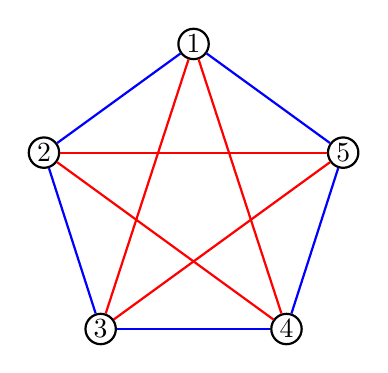
\begin{tikzpicture}
			\tikzset{punkt/.style={circle, thick, draw=black, minimum width=0.2cm,inner sep=1}}
			\node[punkt] at (0.0, 2.0) (a) {$1$};
			\node[punkt] at (-1.9, 0.62) (b) {$2$};
			\node[punkt] at (-1.18, -1.62) (c) {$3$};
			\node[punkt] at (1.18, -1.62) (d) {$4$};
			\node[punkt] at (1.9, 0.62) (e) {$5$};
			%\draw (0,0) circle [radius=2];

			% Blue edges
			\draw [thick, draw=blue] (a) -- (b);
			\draw [thick, draw=blue] (b) -- (c);
			\draw [thick, draw=blue] (c) -- (d);
			\draw [thick, draw=blue] (d) -- (e);
			\draw [thick, draw=blue] (e) -- (a);

			% Red edges
			\draw [thick, draw=red] (a) -- (c);
			\draw [thick, draw=red] (a) -- (d);
			\draw [thick, draw=red] (b) -- (d);
			\draw [thick, draw=red] (b) -- (e);
			\draw [thick, draw=red] (c) -- (e);
		\end{tikzpicture}
		\caption{A 2-edge coloring on $K_{5}$ that admits no monochromatic subclique of order $3$.}
		\label{fig:K5_counter_example}
	\end{figure}
	Finally since $R(3, 3) > 5$ and $R(3, 3) \leq 6$, we obtain that $R(3, 3) = 6$.
\end{example}
\newpage

We might also be interested in when an $r$-edge coloring of a complete graph admits some special monochromatic subgraphs, following this spirit we introduce the following definition:
\begin{definition}
	Let $G_1, G_2, \ldots, G_r$ be graphs, the \textit{generalized Ramsey number} $R(G_1, G_2, \ldots, G_{r})$ is the smallest integer $N$ such that for any $r$-edge coloring $\chi: E(K_N) \to \{c_1, c_2, \ldots, c_{r}\}$ there exists some index $i \in [1; r]$ such that there exists a $c_i$ monochromatic subgraph of $K_n$ which is isomorphic to $G_{i}$.
\end{definition}

It is worth noting that the generalized Ramsey number $R(G_1, G_2, \ldots, G_{r})$ is well defined. This can be seen as follows: let $\ell_j = \abs{V(G_{j})}$ consider the arbitrary $r$-coloring $\chi: E(K_n) \to \{c_1, c_2, \ldots, c_{r}\}$ of $K_n$ with $n = R(\ell_1, \ell_2, \ldots, \ell_{r})$. Then by the definition of $R(\ell_1, \ell_2, \ldots, \ell_{r})$ there exists an $i \in [1; r]$ such that $\chi$ admits a $c_i$-monochromatic clique of order $\ell_i$. The rest follows by the well ordering principle and the fact that $G_i$ is isomorphic to a subgraph of the previously mentioned $c_{i}$-monochromatic clique.

\section{Upper Bounds}\label{sec:upper_bound}
In this section we will prove several upper bounds for both regular and generalized Ramsey numbers, we will start by proving the following upper bound for $R(G_1, G_2, \ldots, G_{r})$.
\begin{theorem}\label{thm:ramsey_upper_bound}
	Let $G_1, G_2, \ldots, G_r$ be graphs with at least $2$ vertices, then:
	\begin{equation*}
		R(G_{1}, G_2, \ldots, G_{r}) \leq 2 - r + \sum_{i = 1}^r R(G_1, \ldots, G_{i - 1}, G_{i}', G_{i + 1}, \ldots, G_{r})
	\end{equation*}
	where the graph $G'$ is obtained from $G$ by deleting one vertex and all of the edges incident to it.
\end{theorem}
\begin{proof}
	For the sake of convenience we will let $R_i = R(G_1, \ldots, G_{i - 1}, G'_{i}, G_{i + 1}, \ldots, G_{r})$ throughout the proof.
	Let $N := 2 - r + \sum_{i = 1}^r R_{i}$ and $\chi$ be an $r$-edge coloring of $K_N$.
	Let $v \in V(K_{N})$, then $v$ is adjacent with $N - 1 = 1 +\sum_{i = 1}^r \left(R_{i} - 1\right)$ other vertices in $K_N$.
	By the Generalized Pigeon Hole Principle (Theorem \ref{thm:gpp}) there exists an $i \in [1; r]$ such that $\abs{\mathcal{N}_{\chi}(v, c_i)} \geq R_{i}$.
	By the definition of $R_i$, we have two cases:
	\begin{enumerate}
		\item Either $\chi$ admits a $c_j$-monochromatic subgraph which is isomorphic with $G_j$, with vertices belonging to $\mathcal{N}_{\chi}(v, c_{i})$, with $j \neq i$, in which case we are done.
		\item Or $\chi$ admits a $c_i$-monochromatic subgraph which is isomorphic with $G'_{i}$ with vertices belonging to $\mathcal{N}_{\chi}(v, c_i)$, of order $\ell_i - 1$, in which case adding $v$ along with the appropriate edges in the set $\left\{\{v, u\} \middle| u \in \mathcal{N}_{\chi}(v, c_{i})\right\}$ forms a $c_i$-monochromatic subgraph which is isomorphic with $G_{i}$. \qedhere
	\end{enumerate}
\end{proof}

In particular Theorem \ref{thm:ramsey_upper_bound}, with $G_i = K_{\ell_{i}}$ implies that:
\begin{equation}\label{eq:cor_1}
	R \left(\ell_1, \ell_2, \ldots, \ell_{r}\right) \leq 2 - r +  \sum_{i = 1}^r R(\ell_1, \ldots, \ell_{i - 1}, \ell_i, \ell_{i + 1}, \ldots, \ell_{r})
\end{equation}

\newpage
\begin{corollary}\label{cor:R3r}
	Let $r \in \mathbb{N}^{+}$ then $R(3; r) \leq 3r!$.
\end{corollary}
\begin{proof}
	We will prove the corollary using induction on $r$. Clearly the result holds in the case where $r = 1$. Next for an arbitrary $r \in \mathbb{N}^{+}$ it follows by Equation \eqref{eq:cor_1}, that:
	\begin{equation}\label{eq:R3r}
		R(3; r) \stackrel{(a)}{\leq} r R(2, 3, \ldots, 3) \stackrel{(b)}{=} r R(3; r - 1) \stackrel{(c)}{=} 3r (r - 1)! = 3r!
	\end{equation}
	where $(a)$ follows by Equation \eqref{eq:R3r}, $(b)$ follows since letting $n := R(2, 3, \ldots, 3)$ we see that every $r$-edge coloring on $K_n$ either admits a monochromatic clique of order $2$ of the appropriate color or we actually have $(r - 1)$-edge coloring on $K_n$. Finally $(c)$ follows directly by the induction hypothesis.
\end{proof}


%\begin{proposition}\label{prop:upper_bounds_form_ramseys_theorem}
%	Let $G, H$ be graphs with $\abs{V(G)}, \abs{V(H)} \geq 2$ and let $G'$ and $H'$ be subgraphs of $G$ and $H$ respectively obtained by deleting a vertex and the appropriate edges, then:
%	\begin{equation*}
%		R(G, H) \leq R(G', H) + R(G, H')
%	\end{equation*}
%\end{proposition}
%We will omit the proof, but note that the basic argument is the same as in the proof of Theorem \ref{thm:ramsey_two_colors}.
The following Corollary is a natural consequence of Theorem \ref{thm:ramsey_upper_bound} and the fact that $R(\ell, 2) = R(2, \ell) = \ell$ for all $\ell \geq 2$.
\begin{corollary}
	Let $\ell, k \in \mathbb{N}$ with $\ell, k \geq 2$, then $R(\ell, k) \leq \binom{\ell + k - 2}{\ell - 1}$
\end{corollary}
\begin{proof}
	We will apply induction on $\ell + k$, in the case where $\ell = 2$ we get that
	\begin{equation*}
		R(\ell, k) = k = \frac{k!}{(k - 1)!} = \binom{k + \ell - 2}{\ell - 1}
	\end{equation*}
	The case where $k = 2$ follows in a similar manner. Next we assume that $\ell, k \geq 3$, then:
	\begin{align*}
		R(\ell, k) \stackrel{(a)}{\leq} R(\ell - 1, k) + R(\ell, k - 1) & \stackrel{(b)}{\leq} \binom{(\ell - 1) + k - 2}{(\ell - 1) - 1} + \binom{\ell + (k - 1) - 2}{\ell - 1} \\
		                                                                & =  \frac{(\ell + k - 3)!}{(\ell - 2)!(k - 1)!} + \frac{(\ell + k - 3)!}{(\ell - 1)!(k - 2)!}           \\
		                                                                & =  \frac{(\ell + k - 3)!((\ell - 1) + (k - 1))}{(\ell - 1)!(k - 1)!}
		= \binom{\ell + k - 2}{\ell - 1}
	\end{align*}
	Where $(a)$ follows by Equation \eqref{eq:cor_1} and $(b)$ directly from the induction hypothesis.
\end{proof}

\begin{corollary}\label{cor:upper_bounds_from_ramseys_theorem_even}
	Let $G, H$ be graphs with at least two edges and let $G'$ and $H'$ be subgraphs of $G$ and $H$ respectively obtained by deleting a vertex and the appropriate edges, then if both $R(G', H)$ and $R(G, H')$ are even, then:
	\begin{equation*}
		R(G, H) \leq R(G', H) + R(G, H') - 1
	\end{equation*}
\end{corollary}
\begin{proof}
	Assume for the sake of contradiction that the inequality does not hold, then by Theorem \ref{thm:ramsey_upper_bound}, we must have $N := R(G, H) = R(G', H) + R(G, H')$ and hence there exists an $2$-edge coloring $\chi: E(K_{N - 1}) \to \left\{red, blue\right\}$ of $K_{N - 1}$ which admits no $red$-monochromatic subgraphs which are isomorphic to $G$ and no $blue$-monochromatic subgraph which are isomorphic to $H$. For all $v \in V(K_{N - 1})$ we thus must have:
	\begin{equation*}
		\abs{\mathcal{N}_{\chi}(v; red)} \leq R(G', H) - 1 \text{ and } \abs{\mathcal{N}_{\chi}(v; blue)} \leq R(G, H') - 1
	\end{equation*}
	since we would otherwise have a $red$(or $blue$)-monochromatic subgraph which is isomorphic to $G$ (or $H$). Next since $v$ is adjacent to $N - 2 = R(G', H) + R(G, H') - 2$ vertices we see that we must have:
	\begin{equation*}
		\abs{\mathcal{N}_{\chi}(v; red)} = R(G', H) - 1 \text{ and } \abs{\mathcal{N}_{\chi}(v; blue)} = R(G, H') - 1
	\end{equation*}
	Next let $k := \abs{\left\{e \in E(K_{N - 1}) | \chi(e) = red\right\}}$ that is $k$ is the number of edges which $\chi$, colors $red$. Thus we may also compute $k$ as:
	\begin{equation}\label{eq:k_is_not_integer}
		k = \frac{1}{2}\sum_{u \in V(K_{N - 1})}\abs{\mathcal{N}_{\chi}(u; red)} = \frac{1}{2}(N - 1)(R(G', H) - 1)
	\end{equation}
	however both $N-1$ and $R(G', H) - 1$ are odd by our assumptions, combining this with Equation \eqref{eq:k_is_not_integer}, implies that $k$ is not natural number a clear contradiction.
\end{proof}

\section{Lower Bounds and the Probabilistic Method}\label{sec:lower_bound}
The probabilistic methodprobability was pioneered by Paul Erdős, and it is generally used throughout combinatorics to establish various lower bounds using methods from probability theory, for graph Ramsey theory it yields some of the best lowerbounds for large Ramsey numbers. Suppose we wish to find a lower bound for $R(\ell_1, \ell_2, \ldots,  \ell_{r})$ the basic idea, at least when applying the method to graph Ramsey theory is to consider a random $r$-edge coloring $\chi$ on a the complete graph $K_{N}$. If the probability, that there exists no indices $i \in [1; r]$ such that $\chi$ admits a $c_{i}$-monochromatic clique of order $\ell_{i}$, is less than $1$, then we must have:
\begin{equation*}
	R(\ell_1, \ell_2, \ldots, \ell_{r}) > N
\end{equation*}
We will need the following lemma, which we state without proof.

\begin{lemma}[Stirlings formula]\label{lem:stirling}
	Let $n \in \mathbb{N}$, then:
	\begin{equation*}
		n! > \sqrt{2 \pi n} \left(\frac{n}{\e}\right)^{n}
	\end{equation*}
\end{lemma}
We now state and prove the main theorem of this section.
\begin{theorem}
	Let $r, \ell \geq 2$, then:
	\begin{equation*}
		R(\ell; r) > \frac{\left(2\pi \ell\right)^{\frac{1}{2\ell}}\ell \sqrt{r}^{\ell}}{r^{\frac{1}{2\ell}}\e}
	\end{equation*}
\end{theorem}
\begin{proof}
	Let $N \geq \ell$ be arbitrary for now. Let $\chi: E(K_N) \to \left\{c_1, c_2, \ldots, c_{r}\right\}$ be a random $r$-edge coloring, with each edge $e$ colored uniformly and independently of the other edges, that is $\mathbb{P}(\chi(e) = c_{i}) = \frac{1}{r}$ for every $i \in [1; r]$. Enumerate the $\ell$-cliques of $K_{N}$ as $C_1, C_2, \ldots, C_{\binom{N}{\ell}}$ and consider the stochastic variables $X_1, X_2, \ldots X_{\binom{N}{\ell}}$ as:
	\begin{equation*}
		X_i = \begin{cases}
			1 & \text{ if } \abs{\chi(E(G \vert_{C_i}))} = 1 \\
			0 & \text{ otherwise }
		\end{cases}
	\end{equation*}
	that is $X_i$ is an indicator function which indicates if the clique $C_i$ is monochromatic under $\chi$. Next notice that
	\begin{equation}\label{eq:prop_mon_clique}
		\mathbb{P}(X_i = 1) = r \cdot \left(\frac{1}{r}\right)^{\binom{\ell}{2}} = r \cdot \left(\frac{\sqrt{r}}{\sqrt{r}^{\ell}}\right)^\ell
	\end{equation}
	since $\abs{E(G \vert_{C_i})} = \binom{\ell}{2} = \frac{\ell^2 - \ell}{2}$. Thus:
	\begin{equation}\label{eq:prob_method}
		\mathbb{E} \left[\sum_{i = 1}^{\binom{N}{\ell}} X_{i}\right]
		= \sum_{i = 1}^{\binom{N}{\ell}} \mathbb{P}(X_i = 1)
		\stackrel{(a)}{\leq} \frac{N^{\ell}}{\ell!} \frac{r}{r^{\binom{\ell}{2}}}
		\stackrel{(b)}{<} \frac{N^{\ell}r}{\sqrt{2\pi \ell} \left(\frac{\ell}{\e}\right)^{\ell}}   \left(\frac{\sqrt{r}}{\sqrt{r}^{\ell}}\right)^{\ell}
		= \frac{r}{\sqrt{2\pi\ell}} \left(\frac{N \e \sqrt{r}}{\ell \sqrt{r}^{\ell}}\right)^{\ell}
	\end{equation}
	where $(a)$ follows by Equation \eqref{eq:prop_mon_clique} and $\frac{N!}{(N - \ell)!} = \prod^N_{k = N - \ell + 1} k < N^{\ell}$ and $(b)$ by Stirlings formula (Lemma \ref{lem:stirling}). \\
	The rest follows as $\frac{r}{\sqrt{2\pi\ell}} \left(\frac{N \e \sqrt{r}}{\ell \sqrt{r}^{\ell}}\right)^{\ell} \geq 1$ if and only if $N \geq \frac{\ell \sqrt{r}^{\ell}}{\e \sqrt{r}} \left(\frac{\sqrt{2\pi\ell}}{r}\right)^{\frac{1}{\ell}}$. Thus since inequality $(b)$ is strict we see that $R(\ell; r) > \frac{\ell \sqrt{r}^{\ell}}{\e \sqrt{r}} \left(\frac{\sqrt{2\pi\ell}}{r}\right)^{\frac{1}{\ell}}$.
	%Now if $\frac{r}{\sqrt{2\pi\ell}} \leq 1$, then setting $N := \frac{\ell\sqrt{r}^{\ell}}{e \sqrt{r}}$ implies $\mathbb{E} \left[\sum_{i = 1}^{\binom{N}{\ell}} X_{i}\right] < 1$, by Equation \eqref{eq:prob_method}, meaning $R(\ell; r) > N$. Alternately if $\frac{r}{\sqrt{2\pi\ell}}$ setting $N := \frac{\ell \sqrt{r}^{\ell}}{\e \sqrt{r}} \left(\frac{\sqrt{2\pi\ell}}{r}\right)^{\frac{1}{\ell}}$, then Equation \eqref{eq:prob_method}, once again gives $\mathbb{E} \left[\sum_{i = 1}^{\binom{N}{\ell}} X_{i}\right] < 1$ concluding the proof.
\end{proof}
%\begin{theorem}
%	Let $\ell \geq 3$ then $R(\ell, \ell) > \frac{\ell}{\e \sqrt{2}} 2^{\ell / 2}$.
%\end{theorem}
%\begin{proof}
%	Let $\chi: E(K_N) \to \left\{red, blue\right\}$ be a random $2$-edge coloring with, we will assume the $\chi(e)$ of is chosen uniformly and independently. Let $C$ be a subgraph of $K_N$ such that $C$ forms a clique and $A_C$ be the event that $\abs{\chi(E(G \vert_{C}))} = 1$, meaning $C$ is monochromatic. Then:
%	\begin{equation*}
%		\mathbb{P}(A_C) = 2 \left(\frac{1}{2} \right)^{\binom{\ell}{2}} = 2^{1 - \binom{\ell}{2}}
%	\end{equation*}
%	since all $\binom{\ell}{2}$ edges of $C$ is must be colored the same color by $\chi$. Let $\mathcal{C}(K_N;\ell)$ be the set of cliques of $K_N$ of order $\ell$, then:
%	\begin{equation*}
%		\mathbb{P} \left(\bigcup_{C \in \mathcal{C}(K_{N}; \ell)} A_{C}\right) \leq \sum_{C \in \mathcal{C}(K_N; \ell)} \mathbb{P}(A_{C}) = \binom{N}{\ell} 2^{1 - \binom{\ell}{2}}
%	\end{equation*}
%	which follows as $\mathcal{C}(K_N; \ell) = \binom{N}{\ell}$. Now if this probability is strictly less than $1$, we must have:
%	\begin{equation*}
%		\mathbb{P}\left(\bigcap_{C \in \mathcal{C}(K_N; \ell)} \overline{A_{C}}\right) = 1 - \mathbb{P} \left(\bigcup_{C \in \mathcal{C}(K_{N}; \ell)} A_{C}\right) \neq 0
%	\end{equation*}
%	where $\overline{A_C}$ is the complement of $A_C$, meaning it is the event that $C$ is not a monochromatic clique. Meaning if this is the case then there must exist a $2$-edge coloring which emits no monochromatic clique of order $\ell$. However it remains to find an integer $N$ such that $\mathbb{P} \left(\bigcup_{C \in \mathcal{C}(K_{N}; \ell)} A_{C}\right) < 1$. We start by computing an upper bound, for the probability that there is at least one monochromatic clique in $K_N$:
%	\begin{equation*}
%		\mathbb{P} \left(\bigcup_{C \in \mathcal{C}(K_{N}; \ell)} A_{C}\right) \leq \binom{N}{\ell} 2^{1 - \binom{\ell}{2}} \stackrel{(a)}{\leq} \frac{N^{\ell}}{\ell!} 2^{1 - \binom{\ell}{2}} \stackrel{(b)}{<} \frac{2}{\sqrt{2\pi \ell}} \left(\frac{\e \sqrt{2} N}{\ell 2^{\ell/2}}\right)^{\ell}
%	\end{equation*}
%	where inequality $(a)$ follow as $\binom{N}{\ell} = \frac{N(N - 1)\cdots(N - \ell + 1)}{\ell!} \leq \frac{N^{\ell}}{\ell!}$ and $(b)$ by Stirlings formula (Lemma \ref{lem:stirling}) and the fact that:
%	\begin{equation*}
%		2^{1 - \binom{\ell}{2}} = 2 \cdot 2^{(-\ell^2 + \ell) / 2} = \frac{2 \cdot \sqrt{2}^{\ell}}{2^{\frac{\ell^2}{2}}}
%	\end{equation*}
%	The rest follows by setting $N = \frac{\ell}{\e \sqrt{2}} 2^{\ell / 2}$.
%\end{proof}

The following theorem are based upon \cite{fg_and_rt}[Theorem 5.5] and gives us our first lower bound for the non-diagonal Ramsey numbers, note that the theorem can also be applied recursively to give a lower bound a general Ramsey number $R(\ell_1, \ell_2, \ldots, \ell_{r})$, via a process similar to the approach used in the proof of Corollary \ref{cor:ramsey_for_arbitarily_many_colors}.
\begin{theorem}
	Let $\ell \geq 2$, there exists a $c_{\ell} > 0$ such that:
	\begin{equation*}
		R(\ell, k) \geq c_{\ell} \left(\frac{k}{\log(k)}\right)^{\frac{\ell - 1}{2}}
	\end{equation*}
	for all $k \geq 2$.
\end{theorem}
We will only give a sketch of the proof.
\begin{proof}[Proof (Sketch)]
	Let $N = \floor{c_{\ell} \left(\frac{k}{\log(k)}\right)^{\frac{\ell - 1}{2}}}$\footnote{Please note that $N$, is not actually fixed, but rahter $N$ depends on $c_{\ell}$.} and $\chi: E(K_N) \to \left\{red, blue\right\}$ be a random $2$-edge coloring on $K_N$, with each edge $e \in E(K_{N})$ colored independently of the others, and with $\mathbb{P}(\chi(e) = red) = \frac{1}{N^{\frac{2}{\ell  - 1}}}$. Next enumerate the $\ell$ and $k$ cliques of $K_N$ as $C_1, C_2, \ldots, C_{\binom{N}{\ell}}$ and $C'_1, C'_2, \ldots, C'_{\binom{N}{k}}$ respectively. We will define the stochastic variables $X_1, X_2, \ldots, X_{\binom{N}{\ell}}$ and $Y_1, Y_2, \ldots, Y_{\binom{N}{k}}$ as:
	\begin{equation*}
		X_i = \begin{cases}
			1 & \text{ if } \chi(E(G \vert_{C_i})) = \left\{red\right\} \\
			0 & \text{ otherwise }
		\end{cases}
	\end{equation*}
	and
	\begin{equation*}
		Y_i = \begin{cases}
			1 & \text{ if } \chi(E(G \vert_{C'_i})) = \left\{blue\right\} \\
			0 & \text{ otherwise }
		\end{cases}
	\end{equation*}
	Letting $p := \mathbb{P}(\chi(e) = red)$ we see that:
	\begin{equation*}
		\mathbb{E} \left[\sum_{i = 1}^{\binom{N}{\ell}} X_i + \sum_{i = 1}^{\binom{N}{k}} Y_{i}\right] \stackrel{a}{=} \binom{N}{\ell} p^{\binom{\ell}{2}} + \binom{N}{k}(1 - p)^{\binom{k}{2}}
	\end{equation*}
	where $(a)$ follows since each edge is colored independently meaning $\mathbb{P} \left(X_i = 1\right) = p^{\binom{\ell}{2}}$ since each of the $\binom{\ell}{2}$ edges in $G \vert_{C_i}$ must be colored $red$ by $\chi$ and similarly $Y_j = 1$ if and only if each edge in $G \vert_{C'_{i}}$ is colored $blue$ by $\chi$. Finally we note that if $c_{\ell}$ is chosen sufficiently small, then $\binom{N}{\ell} p^{\binom{\ell}{2}} + \binom{N}{k}(1 - p)^{\binom{k}{2}} < 1$.
\end{proof}

\section{Exact Values of Small Ramsey Numbers}\label{sec:exact_values}
In this section we compute the exact values of some of the smaller ramsey numbers, using some of the upper bounds which we proved in Section \ref{sec:upper_bound}. The section will be based upon \cite{emogrt}[Chapter 2].
\begin{theorem}\label{thm:small_ramsey_numbers}
	$R(3, 4) = 9, R(3, 5) = 14$ and $R(4, 4) = 18$.
\end{theorem}
\begin{proof}
	by Corollary \ref{cor:upper_bounds_from_ramseys_theorem_even}, we have:
	\begin{equation}\label{eq:R3_4}
		R(3, 4) \leq R(2, 4) + R(3, 3) - 1 = 9
	\end{equation}
	since $R(2, 4) = 4$ and $R(3, 3) = 6$ by Example \ref{exmp:R3_3}. More over by Theorem \ref{thm:ramsey_upper_bound} and Equation \eqref{eq:R3_4} we have:
	\begin{equation}\label{eq:R3_5}
		R(3, 5) \leq R(2, 5) + R(3, 4) \leq 5 + 9 = 14
	\end{equation}
	If we can construct a $2$-edge coloring $\chi: E(K^{*}_{13}) \to \left\{red, blue\right\}$ on $K^{*}_{13}$ with no $red$-clique of order $3$ and no $blue$ clique of order $5$, then we may conclude that $R(3, 5) = 14$ and hence $R(3, 4) = 9$ by Equations \eqref{eq:R3_4} and \eqref{eq:R3_5}. It is in fact the case that we may construct such a $2$-edge coloring $\chi$ on $K^{*}_{13}$ one example of such a coloring is:
	\begin{equation*}
		\chi(\{i, j\}) = \begin{cases}
			red  & \text{ if } [i - j]_{13} \in \left\{1, 5, 8, 12\right\} \\
			blue & \text{ otherwise }
		\end{cases}
	\end{equation*}
	Please note that $\chi$ is well defined since $-1 \equiv 12 \mod 13$ and $-5 \equiv 8 \mod 13$ and hence $[i - j]_{13} \in \left\{1, 5, 8, 12\right\}$ if and only if $[j - i]_{13} \in \left\{1, 5, 8, 12\right\}$. The fact that $\chi$ admits no $red$-monochromatic cliques of order $3$ and no $blue$-monochromatic cliques of order $5$ is checked via the code in Appendix \ref{app:ramsey_code}.
	Additionally since $R(3, 4) = 14$ we have $R(4, 4) \leq R(3, 4) + R(4, 3) = 18$, once again by Theorem \ref{thm:ramsey_upper_bound}, using this inequality we can show that $R(4, 4) = 18$ by constructing a $2$-edge coloring $\gamma: E(K^{*}_{17}) \to \left\{red, blue\right\}$ which admits no $red$ or $blue$ monochromatic cliques of order $4$. One such $2$-edge coloring is given below:
	\begin{equation*}
		\gamma(\left\{i, j\right\}) = \begin{cases}
			red  & \text{ if } [i -  j]_{17} \in \left\{1, 2, 4, 8, 9, 13, 15, 16\right\} \\
			blue & otherwise
		\end{cases}
	\end{equation*}
	again please note that $\gamma$ is well defined, just like $\chi$, by an identical argument. Again the fact that $\gamma$ admits no $red$ or $blue$ monochromatic cliques of order $5$ is checked via the code in Appendix \ref{app:ramsey_code}.
\end{proof}

For the sake of illustration $K^{*}_{13}$ equiped with the $2$-edge coloring $\chi$ and $K^{*}_{17}$ equiped with the $2$-edge coloring $\gamma$, both from the proof of Theorem \ref{thm:small_ramsey_numbers} is illustated below in Figures \ref{fig:small_ramsey_graphs}
\begin{figure}[H]
	\begin{subfigure}[c]{0.4\textwidth}
		\centering
		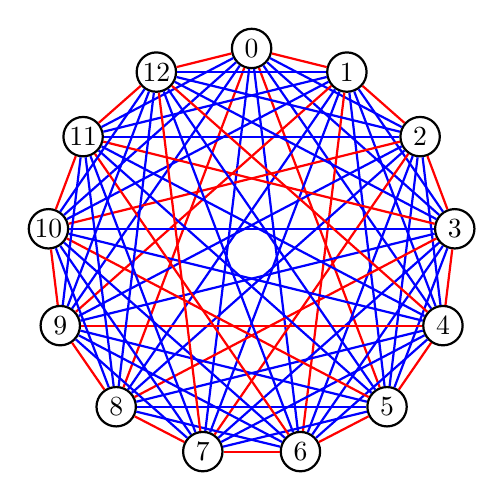
\begin{tikzpicture}
			\tikzset{punkt/.style={circle, thick, draw=black, minimum width=0.5cm,inner sep=0.2}}

			\node[punkt] at (0.0, 2.6) (a) {$0$};
			\node[punkt] at (1.21, 2.3) (b) {$1$};
			\node[punkt] at (2.14, 1.48) (c) {$2$};
			\node[punkt] at (2.58, 0.31) (d) {$3$};
			\node[punkt] at (2.43, -0.92) (e) {$4$};
			\node[punkt] at (1.72, -1.95) (f) {$5$};
			\node[punkt] at (0.62, -2.52) (g) {$6$};
			\node[punkt] at (-0.62, -2.52) (h) {$7$};
			\node[punkt] at (-1.72, -1.95) (i) {$8$};
			\node[punkt] at (-2.43, -0.92) (j) {$9$};
			\node[punkt] at (-2.58, 0.31) (k) {$10$};
			\node[punkt] at (-2.14, 1.48) (l) {$11$};
			\node[punkt] at (-1.21, 2.3) (m) {$12$};
			\draw [thick, draw=red] (a) -- (b);
			\draw [thick, draw=blue] (a) -- (c);
			\draw [thick, draw=blue] (a) -- (d);
			\draw [thick, draw=blue] (a) -- (e);
			\draw [thick, draw=red] (a) -- (f);
			\draw [thick, draw=blue] (a) -- (g);
			\draw [thick, draw=blue] (a) -- (h);
			\draw [thick, draw=red] (a) -- (i);
			\draw [thick, draw=blue] (a) -- (j);
			\draw [thick, draw=blue] (a) -- (k);
			\draw [thick, draw=blue] (a) -- (l);
			\draw [thick, draw=red] (a) -- (m);
			\draw [thick, draw=red] (b) -- (c);
			\draw [thick, draw=blue] (b) -- (d);
			\draw [thick, draw=blue] (b) -- (e);
			\draw [thick, draw=blue] (b) -- (f);
			\draw [thick, draw=red] (b) -- (g);
			\draw [thick, draw=blue] (b) -- (h);
			\draw [thick, draw=blue] (b) -- (i);
			\draw [thick, draw=red] (b) -- (j);
			\draw [thick, draw=blue] (b) -- (k);
			\draw [thick, draw=blue] (b) -- (l);
			\draw [thick, draw=blue] (b) -- (m);
			\draw [thick, draw=red] (c) -- (d);
			\draw [thick, draw=blue] (c) -- (e);
			\draw [thick, draw=blue] (c) -- (f);
			\draw [thick, draw=blue] (c) -- (g);
			\draw [thick, draw=red] (c) -- (h);
			\draw [thick, draw=blue] (c) -- (i);
			\draw [thick, draw=blue] (c) -- (j);
			\draw [thick, draw=red] (c) -- (k);
			\draw [thick, draw=blue] (c) -- (l);
			\draw [thick, draw=blue] (c) -- (m);
			\draw [thick, draw=red] (d) -- (e);
			\draw [thick, draw=blue] (d) -- (f);
			\draw [thick, draw=blue] (d) -- (g);
			\draw [thick, draw=blue] (d) -- (h);
			\draw [thick, draw=red] (d) -- (i);
			\draw [thick, draw=blue] (d) -- (j);
			\draw [thick, draw=blue] (d) -- (k);
			\draw [thick, draw=red] (d) -- (l);
			\draw [thick, draw=blue] (d) -- (m);
			\draw [thick, draw=red] (e) -- (f);
			\draw [thick, draw=blue] (e) -- (g);
			\draw [thick, draw=blue] (e) -- (h);
			\draw [thick, draw=blue] (e) -- (i);
			\draw [thick, draw=red] (e) -- (j);
			\draw [thick, draw=blue] (e) -- (k);
			\draw [thick, draw=blue] (e) -- (l);
			\draw [thick, draw=red] (e) -- (m);
			\draw [thick, draw=red] (f) -- (g);
			\draw [thick, draw=blue] (f) -- (h);
			\draw [thick, draw=blue] (f) -- (i);
			\draw [thick, draw=blue] (f) -- (j);
			\draw [thick, draw=red] (f) -- (k);
			\draw [thick, draw=blue] (f) -- (l);
			\draw [thick, draw=blue] (f) -- (m);
			\draw [thick, draw=red] (g) -- (h);
			\draw [thick, draw=blue] (g) -- (i);
			\draw [thick, draw=blue] (g) -- (j);
			\draw [thick, draw=blue] (g) -- (k);
			\draw [thick, draw=red] (g) -- (l);
			\draw [thick, draw=blue] (g) -- (m);
			\draw [thick, draw=red] (h) -- (i);
			\draw [thick, draw=blue] (h) -- (j);
			\draw [thick, draw=blue] (h) -- (k);
			\draw [thick, draw=blue] (h) -- (l);
			\draw [thick, draw=red] (h) -- (m);
			\draw [thick, draw=red] (i) -- (j);
			\draw [thick, draw=blue] (i) -- (k);
			\draw [thick, draw=blue] (i) -- (l);
			\draw [thick, draw=blue] (i) -- (m);
			\draw [thick, draw=red] (j) -- (k);
			\draw [thick, draw=blue] (j) -- (l);
			\draw [thick, draw=blue] (j) -- (m);
			\draw [thick, draw=red] (k) -- (l);
			\draw [thick, draw=blue] (k) -- (m);
			\draw [thick, draw=red] (l) -- (m);
		\end{tikzpicture}
		\caption{The $2$-edge coloring $\chi$ on $K^{*}_{13}$}
	\end{subfigure}
	\begin{subfigure}[c]{0.6\textwidth}
		\centering
		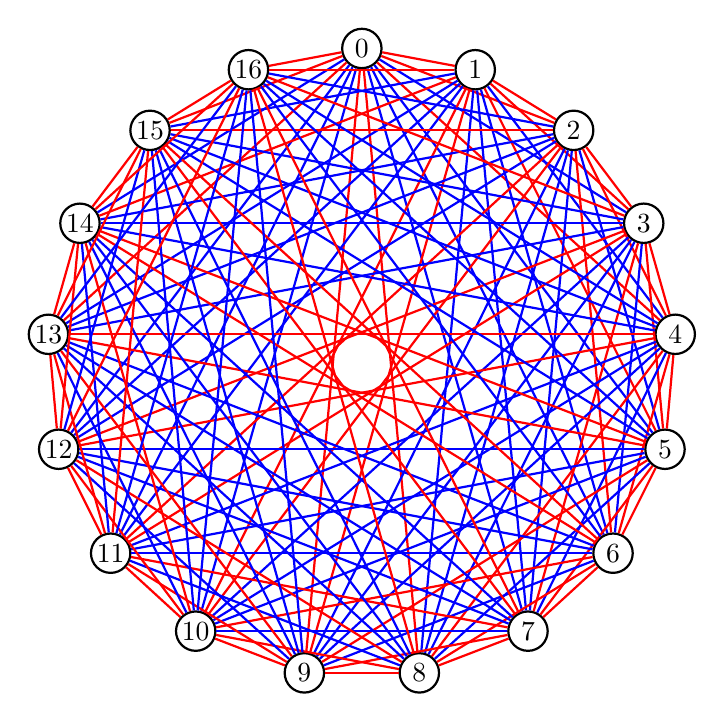
\begin{tikzpicture}
			\tikzset{punkt/.style={circle, thick, draw=black, minimum width=0.5cm,inner sep=0.2}}
			\node[punkt] at (0.0, 4.0) (a) {$0$};
			\node[punkt] at (1.44, 3.73) (b) {$1$};
			\node[punkt] at (2.69, 2.96) (c) {$2$};
			\node[punkt] at (3.58, 1.78) (d) {$3$};
			\node[punkt] at (3.98, 0.37) (e) {$4$};
			\node[punkt] at (3.85, -1.09) (f) {$5$};
			\node[punkt] at (3.19, -2.41) (g) {$6$};
			\node[punkt] at (2.11, -3.4) (h) {$7$};
			\node[punkt] at (0.73, -3.93) (i) {$8$};
			\node[punkt] at (-0.73, -3.93) (j) {$9$};
			\node[punkt] at (-2.11, -3.4) (k) {$10$};
			\node[punkt] at (-3.19, -2.41) (l) {$11$};
			\node[punkt] at (-3.85, -1.09) (m) {$12$};
			\node[punkt] at (-3.98, 0.37) (n) {$13$};
			\node[punkt] at (-3.58, 1.78) (o) {$14$};
			\node[punkt] at (-2.69, 2.96) (p) {$15$};
			\node[punkt] at (-1.44, 3.73) (q) {$16$};
			\draw [thick, draw=red] (a) -- (b);
			\draw [thick, draw=red] (a) -- (c);
			\draw [thick, draw=blue] (a) -- (d);
			\draw [thick, draw=red] (a) -- (e);
			\draw [thick, draw=blue] (a) -- (f);
			\draw [thick, draw=blue] (a) -- (g);
			\draw [thick, draw=blue] (a) -- (h);
			\draw [thick, draw=red] (a) -- (i);
			\draw [thick, draw=red] (a) -- (j);
			\draw [thick, draw=blue] (a) -- (k);
			\draw [thick, draw=blue] (a) -- (l);
			\draw [thick, draw=blue] (a) -- (m);
			\draw [thick, draw=red] (a) -- (n);
			\draw [thick, draw=blue] (a) -- (o);
			\draw [thick, draw=red] (a) -- (p);
			\draw [thick, draw=red] (a) -- (q);
			\draw [thick, draw=red] (b) -- (c);
			\draw [thick, draw=red] (b) -- (d);
			\draw [thick, draw=blue] (b) -- (e);
			\draw [thick, draw=red] (b) -- (f);
			\draw [thick, draw=blue] (b) -- (g);
			\draw [thick, draw=blue] (b) -- (h);
			\draw [thick, draw=blue] (b) -- (i);
			\draw [thick, draw=red] (b) -- (j);
			\draw [thick, draw=red] (b) -- (k);
			\draw [thick, draw=blue] (b) -- (l);
			\draw [thick, draw=blue] (b) -- (m);
			\draw [thick, draw=blue] (b) -- (n);
			\draw [thick, draw=red] (b) -- (o);
			\draw [thick, draw=blue] (b) -- (p);
			\draw [thick, draw=red] (b) -- (q);
			\draw [thick, draw=red] (c) -- (d);
			\draw [thick, draw=red] (c) -- (e);
			\draw [thick, draw=blue] (c) -- (f);
			\draw [thick, draw=red] (c) -- (g);
			\draw [thick, draw=blue] (c) -- (h);
			\draw [thick, draw=blue] (c) -- (i);
			\draw [thick, draw=blue] (c) -- (j);
			\draw [thick, draw=red] (c) -- (k);
			\draw [thick, draw=red] (c) -- (l);
			\draw [thick, draw=blue] (c) -- (m);
			\draw [thick, draw=blue] (c) -- (n);
			\draw [thick, draw=blue] (c) -- (o);
			\draw [thick, draw=red] (c) -- (p);
			\draw [thick, draw=blue] (c) -- (q);
			\draw [thick, draw=red] (d) -- (e);
			\draw [thick, draw=red] (d) -- (f);
			\draw [thick, draw=blue] (d) -- (g);
			\draw [thick, draw=red] (d) -- (h);
			\draw [thick, draw=blue] (d) -- (i);
			\draw [thick, draw=blue] (d) -- (j);
			\draw [thick, draw=blue] (d) -- (k);
			\draw [thick, draw=red] (d) -- (l);
			\draw [thick, draw=red] (d) -- (m);
			\draw [thick, draw=blue] (d) -- (n);
			\draw [thick, draw=blue] (d) -- (o);
			\draw [thick, draw=blue] (d) -- (p);
			\draw [thick, draw=red] (d) -- (q);
			\draw [thick, draw=red] (e) -- (f);
			\draw [thick, draw=red] (e) -- (g);
			\draw [thick, draw=blue] (e) -- (h);
			\draw [thick, draw=red] (e) -- (i);
			\draw [thick, draw=blue] (e) -- (j);
			\draw [thick, draw=blue] (e) -- (k);
			\draw [thick, draw=blue] (e) -- (l);
			\draw [thick, draw=red] (e) -- (m);
			\draw [thick, draw=red] (e) -- (n);
			\draw [thick, draw=blue] (e) -- (o);
			\draw [thick, draw=blue] (e) -- (p);
			\draw [thick, draw=blue] (e) -- (q);
			\draw [thick, draw=red] (f) -- (g);
			\draw [thick, draw=red] (f) -- (h);
			\draw [thick, draw=blue] (f) -- (i);
			\draw [thick, draw=red] (f) -- (j);
			\draw [thick, draw=blue] (f) -- (k);
			\draw [thick, draw=blue] (f) -- (l);
			\draw [thick, draw=blue] (f) -- (m);
			\draw [thick, draw=red] (f) -- (n);
			\draw [thick, draw=red] (f) -- (o);
			\draw [thick, draw=blue] (f) -- (p);
			\draw [thick, draw=blue] (f) -- (q);
			\draw [thick, draw=red] (g) -- (h);
			\draw [thick, draw=red] (g) -- (i);
			\draw [thick, draw=blue] (g) -- (j);
			\draw [thick, draw=red] (g) -- (k);
			\draw [thick, draw=blue] (g) -- (l);
			\draw [thick, draw=blue] (g) -- (m);
			\draw [thick, draw=blue] (g) -- (n);
			\draw [thick, draw=red] (g) -- (o);
			\draw [thick, draw=red] (g) -- (p);
			\draw [thick, draw=blue] (g) -- (q);
			\draw [thick, draw=red] (h) -- (i);
			\draw [thick, draw=red] (h) -- (j);
			\draw [thick, draw=blue] (h) -- (k);
			\draw [thick, draw=red] (h) -- (l);
			\draw [thick, draw=blue] (h) -- (m);
			\draw [thick, draw=blue] (h) -- (n);
			\draw [thick, draw=blue] (h) -- (o);
			\draw [thick, draw=red] (h) -- (p);
			\draw [thick, draw=red] (h) -- (q);
			\draw [thick, draw=red] (i) -- (j);
			\draw [thick, draw=red] (i) -- (k);
			\draw [thick, draw=blue] (i) -- (l);
			\draw [thick, draw=red] (i) -- (m);
			\draw [thick, draw=blue] (i) -- (n);
			\draw [thick, draw=blue] (i) -- (o);
			\draw [thick, draw=blue] (i) -- (p);
			\draw [thick, draw=red] (i) -- (q);
			\draw [thick, draw=red] (j) -- (k);
			\draw [thick, draw=red] (j) -- (l);
			\draw [thick, draw=blue] (j) -- (m);
			\draw [thick, draw=red] (j) -- (n);
			\draw [thick, draw=blue] (j) -- (o);
			\draw [thick, draw=blue] (j) -- (p);
			\draw [thick, draw=blue] (j) -- (q);
			\draw [thick, draw=red] (k) -- (l);
			\draw [thick, draw=red] (k) -- (m);
			\draw [thick, draw=blue] (k) -- (n);
			\draw [thick, draw=red] (k) -- (o);
			\draw [thick, draw=blue] (k) -- (p);
			\draw [thick, draw=blue] (k) -- (q);
			\draw [thick, draw=red] (l) -- (m);
			\draw [thick, draw=red] (l) -- (n);
			\draw [thick, draw=blue] (l) -- (o);
			\draw [thick, draw=red] (l) -- (p);
			\draw [thick, draw=blue] (l) -- (q);
			\draw [thick, draw=red] (m) -- (n);
			\draw [thick, draw=red] (m) -- (o);
			\draw [thick, draw=blue] (m) -- (p);
			\draw [thick, draw=red] (m) -- (q);
			\draw [thick, draw=red] (n) -- (o);
			\draw [thick, draw=red] (n) -- (p);
			\draw [thick, draw=blue] (n) -- (q);
			\draw [thick, draw=red] (o) -- (p);
			\draw [thick, draw=red] (o) -- (q);
			\draw [thick, draw=red] (p) -- (q);
		\end{tikzpicture}
		\caption{The $2$-edge coloring $\gamma$ on $K^{*}_{17}$}
	\end{subfigure}
	\caption{The two 2-edge colorings described in the proof of Theorem \ref{thm:small_ramsey_numbers} illustrated.}
	\label{fig:small_ramsey_graphs}
\end{figure}


Before moving on we will need one additional concept, introduced in the following definition:
\begin{definition}\label{def:set_sum_free}
	Let $(G, +)$ be an abelian group, then the subset $S \subseteq G$ is called \textit{sum-free} if the equation $x + y = z$ has no solution in $S$.
\end{definition}

Some parts of the proof of the following Theorem is inspired by \cite{graph_theory}[Exercise 12.3.4]
\begin{theorem}\label{thm:R3_3_3}
	We have $R(3, 3, 3) = 17$.
\end{theorem}
\begin{proof}
	We start by showing that any $3$-edge coloring $\chi: E(K_{17}) \to \left\{red, blue, green\right\}$ admits a monochromatic clique of order $3$. Let $v \in V(K_{17})$, by the generalized pigeonhole principle (Theorem \ref{thm:gpp}), there exists a color $c \in \left\{red, blue, green\right\}$ such that $\abs{\mathcal{N}_{\chi}(v; c)} \geq 6$. Assume without loss of generalization that $c = red$, then we may assume that $\chi\left(E(K_{17} \vert_{\mathcal{N}_{\chi}(v; c)})\right) = \left\{blue, green\right\}$, otherwise we would have a $red$-monochromatic clique of order $3$. However since $R(3, 3) = 6$, this means that $\chi$ admits either a $blue$ or $green$ monochromatic clique of order $3$.

	Next we will show that $R(3, 3, 3) > 16$, we will do this by constructing a $3$-edge coloring $\gamma$ on the complete graph $K$ with vertex set $\mathbb{Z}_2[X] / \gen{X^4 + X + 1}$\footnote{Which is of course isomorphic to $\mathbb{F}_{16}$, however it will be move convinient for us to work from this polynomial view.}. We will construct $3$ cosets $S_{red}, S_{blue}, S_{green}$ which partition $\mathbb{Z}_2[X] / \gen{X^4 + X + 1}$, and assign a color to the edge $\left\{v, u\right\}$ according to which coset $v + u$ belongs to. To start let:
	\begin{equation*}
		S_{red} := \left\{X^3, X^2 + X^{3}, X + X^{3}, 1 + X + X^2 + X^3 , 1\right\}
	\end{equation*}
	Note that $S_{red}$ is a subgroup of the multiplicative group $(\mathbb{Z}_2[X] / \gen{X^4 + X + 1})^{*}$, additionally we note that $S_{red}$ is sum-free, which is easy albeit cumbersome to check. Similarly we let $A_{blue} := X S_{red}$ and $S_{green} := X^2 S_{red}$, these cosets must also be sum-free since $a + b = c$ with $a, b, c \in S_{blue}$ or $a, b, c \in S_{green}$ would imply:
	\begin{equation*}
		Xa' + Xb' = Xc' \implies a' + b' = c' \text{ with } a', b', c' \in S_{red}
	\end{equation*}
	or
	\begin{equation*}
		X^{2}a' + X^{2}b' = X^{2}c' \implies a' + b' = c' \text{ with } a', b', c' \in S_{red}
	\end{equation*}
	respectively, since $\mathbb{Z}_2[X] / \gen{X^4 + X + 1}$ is a finite field and hence a domain. Define $\gamma(\left\{v, u\right\}) = c$ if and only if $v + u \in S_{c}$, additionally we note that $\gamma$ is well defined as $v \neq u$ and $\Char(\mathbb{Z}_2[X] / \gen{X^4 + X + 1}) = 2$. Assume for the sake of contradiction that $\gamma$ admits a $c$-monochromatic clique of order $3$, that is there exists $u, v, w \in V(K) = \mathbb{Z}_2[X] / \gen{X^4 + X + 1}$ such that $u + v, u + w, v + w \in S_c$, then $u + w = (u + v) + (v + w)$ contradicting the fact that $S_c$ is sum-free.
\end{proof}

Finally we present a summary of the exact values and bounds for small Ramsey numbers, below in Table \ref{tab:small_values}:
\begin{table}[H]
	\centering
	\begin{tabular} {||c|c|c|c|c||}
		\hline
		$\ell_1 \setminus \ell_{2}$ & $2$ & $3$  & $4$                     & $5$                      \\
		\hline
		$2$                         & $2$ & $3$  & $4$                     & $5$                      \\
		\hline
		$3$                         & $3$ & $6$  & $9$                     & $14$                     \\
		\hline
		$4$                         & $4$ & $9$  & $18$                    & $\leq31$, $\mathbf{25}$  \\
		\hline
		$5$                         & $5$ & $14$ & $\leq31$, $\mathbf{25}$ & $\leq62$, \textbf{43-48} \\
		\hline
	\end{tabular}
	\caption{Some exact values and bounds for small Ramsey numbers. The bold entries are exact values or best known bounds, if the exact value is unknown, which we have not covered in this project. The bold values are sourced from \cite{small_values}.}
	\label{tab:small_values}
\end{table}

\section{Asymptotic Behaviour of Certain Ramsey Numbers}\label{sec:ass_ramsey}
In this section we will investigate the asymptotic behaviour of certain Ramsey numbers. Starting with $R(\ell; r)$ as $r \to \infty$ and finishing providing an explicit construction using projective planes, which shows that $R(3, \ell) = \Omega(\ell^{3 / 2})$.
\subsection{Asymptotic Behaviour of $R(\ell; r)$ as $r \to \infty$}\label{sec:ramsey_ass}
In this subsection we will briefly investigate the asymptotic behaviour of $R(\ell; r)$ as $r \to \infty$, with $\ell \geq 3$, our primary reference will be \cite{emogrt}[Subsection 2.3]. We will not consider the case where $\ell = 2$, since $R(2; r) = 2$ for all $r \in \mathbb{N}^{+}$.

\begin{definition}
	Let $f: \mathbb{N} \to \mathbb{R}^{+}$, then $f$ is called \textit{super-multiplicative} if
	\begin{equation*}
		f(n + m) \geq f(m)f(n)
	\end{equation*}
	for all $n,m \in \mathbb{N}^{+}$.
\end{definition}

\begin{lemma}\label{lem:limit_of_super_multiplicative}
	Let $f: \mathbb{N} \to \mathbb{R}^{+}$ be a super-multiplicative function, then the limit of $f(k)^{1 / k}$ as $k \to \infty$ exists an is equal to $\sup_{k \in \mathbb{N}^{+}} f(k)^{1 / k}$. Furthermore if $m \in \mathbb{N}^{+}$ is fixed, then there exists some constant $c_m > 0$ such that:
	\begin{equation*}
		f(n) \geq c_{m} f(m)^{n / m}
	\end{equation*}
	for all $n \geq m$.
\end{lemma}
\begin{proof}
	We clearly have $\limsup_{k \to \infty} f(k)^{1/k} \leq \sup_{k \in \mathbb{N}^{+}} f(k)^{1/k}$, next we will show that $\liminf_{k \to \infty} f(k)^{1 / k} \geq \sup_{k \in \mathbb{N}^{+}} f(k)^{1/k}$, by considering two distinct cases, namely $\sup_{k \in \mathbb{N}^{+}} f(k)^{1/k} < \infty$ and $\sup_{k \in \mathbb{N}^{+}} f(k)^{1/k} = \infty$, separately:
	\begin{enumerate}
		\item If $\sup_{k \in \mathbb{N}^{+}} f(k)^{1/k} < \infty$, then for all $\varepsilon > 0$ there exists an $m \in \mathbb{N}^{+}$ such that:
		      \begin{equation*}
			      f(m)^{1/m} > \sup_{k \in \mathbb{N}^{+}} f(k)^{1/k} - \varepsilon
		      \end{equation*}
		      by the definition of $\sup_{k \in \mathbb{N}^+} f(k)^{1/k}$. Let $n \geq m$, then there exists $q, r \in \mathbb{N}$ with $0 \leq r < m$ such that $n = qm + r$ thus:
		      \begin{equation*}
			      f(n) \geq f(qm) f(r) \geq f(m)^q f(r)
		      \end{equation*}
		      Since $f$ is a super-multiplicative function. We note that $q / n \to 1 / m$ and $f(r)^{1/n} \to 1$ as $n \to \infty$, and hence:
		      \begin{equation*}
			      \liminf_{k \to \infty} f(k)^{1/k} \geq f(m)^{1/m} > \sup_{k \in \mathbb{N}^{+}} f(k)^{1/k} - \varepsilon
		      \end{equation*}
		      However $\varepsilon > 0$ was arbitrary and hence we must have:
		      \begin{equation*}
			      \liminf_{k \to \infty} f(k)^{1/k} \geq \sup_{k \in \mathbb{N}^{+}} f(k)^{1/k}
		      \end{equation*}
		      and thus:
		      \begin{equation*}
			      \sup_{k \in \mathbb{N}^{+}} f(k)^{1/k} \leq \liminf_{k \to \infty} f(k)^{1/k} \leq \limsup_{k \to \infty} f(k)^{1/k} \leq \sup_{k \in \mathbb{N}^{+}} f(k)^{1/k}
		      \end{equation*}
		      since $\liminf_{k \to \infty} x_{n} \leq \limsup_{k \to \infty} x_{n}$ for every real sequence $\left\{x_k\right\}_{k = 1}^{\infty}$. Meaning
		      \begin{equation*}
			      \liminf_{k\to \infty} f(k)^{1/k} = \limsup_{k \to \infty} f(k)^{1/k} = \sup_{k \in \mathbb{N}^+} f(k)^{1/k}
		      \end{equation*}
		\item If $\sup_{k \in \mathbb{N}^{+}} f(k)^{1/k} = \infty$, then for every $M > 0$ there exists some $m \in \mathbb{N}^{+}$ such that $f(m)^{1/m} > M$, by writing $n \geq m$ as $n = qm + r$, again for suitable $q, r \in \mathbb{N}$ and repeating the same argument we get that:
		      \begin{equation*}
			      \liminf_{k \to \infty} f(k)^{1/k} \geq f(m)^{1/m} > M
		      \end{equation*}
		      Meaning $\liminf_{k \to \infty} f(k)^{1/k} = \infty$.
	\end{enumerate}
	Finally we will show that if $m \in \mathbb{N}^{+}$ is fixed, then there exists a constant $c_m > 0$ such that $f(n) \geq c_{m} f(m)^{n / m}$ for all $n \geq m$. Once again we may write $n = qm + r$ for suitable $q, r \in \mathbb{N}$ such that $0 \leq r < m$. Then:
	\begin{equation*}
		f(n) \geq f(qm) f(r) \geq f(m)^q f(r) \stackrel{(a)}{=} f(m)^{(n - r) / m} f(r) = \frac{f(r)}{f(m)^{r / m}} f(m)^{n / m}
	\end{equation*}
	The rest follows by setting $c_m := \min \left\{\frac{f(r)}{f(m)^{r / m}} \middle| 0 \leq r \leq m\right\}$, notice that $c_m \neq 0$, singe $f$ is strictly positive.
\end{proof}

We now reach the main result of this subsection.
\begin{proposition}\label{prop:r_ell_k_is_super_multiplicative}
	Let $\ell \geq 3$, then the function $r \mapsto R(\ell; r) - 1$ is super-multiplicative. In particular $\lim_{r \to \infty} \left(R(\ell; r) - 1\right)^{1/r} = \sup_{r \in \mathbb{N}} (R(\ell; r) - 1)^{1 / r}$ and for every $r \in \mathbb{N}^{+}$ there exists a constant $c_r > 0$ such that $R(\ell; r') \geq c_r R(\ell; r)^{r' / r}$ for all $r' \geq r$.
\end{proposition}

The proof of Proposition \ref{prop:r_ell_k_is_super_multiplicative} will use a technique which is normally refereed to as ``blowing-up'' an $r_1$-edge coloring $\chi$ using another $r_2$-edge coloring $\gamma$, on two complete graphs $K_{1}$ and $K_{2}$ respectively. The process creates an $(r_1 + r_2)$-edge coloring $\psi$ on a complete graph with $\abs{V(K_1)} \cdot \abs{V(K_{2})}$ verticies.
Intuitively the process is the following:
We replace each vertex $u \in V(K_{1})$ with a copy of $K_{2}$, denoted by $K_{2}^{(u)}$, with the edges in $K_2^{(u)}$ colored according to $\gamma$, and color the edges joining the verticies in $K_2^{(v)}$ and $K_2^{(w)}$ the same color as $\left\{v, w\right\}$ under $\chi$.

\begin{proof}[Proof of Proposition \ref{prop:r_ell_k_is_super_multiplicative}]
	Let $r_{1}, r_2 \in \mathbb{N}^{+}$ with $r_1, r_2 \geq 2$, let $n = R(\ell; r_{1}) - 1$ and $m = R(\ell; r_{2}) - 1$. Let $\chi$ and $\gamma$, be a $r_{1}$-edge-coloring or a $r_2$-edge-coloring on the complete graphs $K_V, K_U$ with vertex sets $V := \left\{v_1, v_2, \ldots, v_{n}\right\}$ and $U := \left\{u_1, u_2, \ldots, u_{m}\right\}$ respectively.
	For the sake of simplicity we will without loss of generalization assume that the codomains of $\chi$ and $\gamma$ are disjoint\footnote{If the codomains are intersecting, simply compose either one of $\chi$ and $\gamma$, with a suitable bijection from its codomain to another finite set of colors.}. We will blow-up $\chi$ using $\gamma$ in order to construct a $(r_1 + r_2)$-edge coloring $\psi$ on the complete graph $K_{W}$ with vertex set $W := \left\{w_{i, j} | i \in [1; n], j \in [1; m]\right\}$ clearly $\abs{W} = nm$. We can construct a $(r_1 + r_2)$-edge coloring $\psi$, which admits no monochromatic cliques of order $\ell$, by blowing up $\chi$ with $\gamma$, since $\chi$ and $\gamma$ admits no monochromatic cliques of order $\ell$\footnote{The intuition here is that we have no cliques of order $\ell$, between copies of $K_{U}$ and no cliques contained within each copy of $K_{U}$, due to the properties of $\chi$ and $\gamma$.}.
	That is by defining $\psi$ as:
	\begin{equation*}
		\psi(\left \{w_{i,j}, w_{i', j'}\right\}) := \begin{cases}
			\chi(\left\{v_{i}, v_{i'}\right\})   & \text{ if } j = j' \\
			\gamma(\left\{u_{j}, u_{j'}\right\}) & otherwise          \\
		\end{cases}
	\end{equation*}
	Hence:
	\begin{equation*}
		R(\ell; r_{1} + r_{2}) - 1 \geq mn = (R(\ell; r_{1}) - 1)(R(\ell; r_{2}) - 1)
	\end{equation*}
	The rest follows directly by Lemma \ref{lem:limit_of_super_multiplicative}.
\end{proof}

\begin{corollary}\label{cor:limit_of_R}
	Let $\ell \geq 3$, then $\lim_{r \to \infty} R(\ell; r)^{1/r} = \sup_{r \in \mathbb{N}^{+}} (R(\ell; r) - 1)^{1/r}$
\end{corollary}
\begin{proof}
	We have $\lim_{r \to \infty} \frac{\left(R(\ell; r) - 1\right)^{1/r}}{R(\ell;r)^{1/r}} = \lim_{r \to \infty} \left(1 -  \frac{1}{R(\ell;r)}\right)^{1 / r} = 1$ since $\lim_{r \to \infty} \frac{1}{R(\ell; r)} = 0$, thus $\lim_{r \to \infty} R(\ell; r) ^{1/r} = \lim_{r \to \infty} \left(R(\ell; r) - 1\right)^{1/r} = \sup_{r \in \mathbb{N}^{+}} (R(\ell; r) - 1)^{1/r}$ by Proposition \ref{prop:r_ell_k_is_super_multiplicative}.
\end{proof}

From Corollary \ref{cor:limit_of_R} we see that:
\begin{equation*}
	\lim_{r \to \infty} R(3; r)^{1 / r} \geq \max \left\{(R(3; 2) - 1)^{1 / 2}, (R(3; 3) - 1)^{1/3}\right\}  = \max \left\{5^{1/2}, 16^{1/3}\right\} \geq \frac{5}{2}
\end{equation*}
Since $R(3, 3) = 6$ and $R(3, 3, 3) = 17$, by Example \ref{exmp:R3_3} and Theorem \ref{thm:R3_3_3}. More over we see that $R(3; r) \geq c_r (5 / 2)^r$, for some constant $c_r > 0$ and all $r \geq 2$ by Lemma \ref{lem:limit_of_super_multiplicative}. In subsection \ref{sub:schur_bounds_and_ass}, we will show that $R(3; r)$ grows even more rapidly, by relating it to a different construct.
Finally we note the following conjecture by Paul Erdős:
\begin{conjecture}[Erdős]\label{conj:erdos_limit}
	The limit of $R(3; r)^{1/r}$ as $r \to \infty$ is infinity.
\end{conjecture}
If Conjecture \ref{conj:erdos_limit} holds, then $\ell \geq 3$ implies that $\lim_{r \to \infty} R(\ell; r)^{1/r} = \infty$ since $R(\ell; r) \geq R(3; r)$.

\subsection{Explicit Constructions for $R(3, \ell)$ as $\ell \to \infty$ using Projective Planes}
Our treatment will be based upon \cite{fg_and_rt}[Chapter 1 and Section 5.2], it is a well known that $R(3; \ell) = \Theta(\ell^2 / \log(t))$, the lower bound was first proven in \cite{R3t}, however proof was based upon the probabilistic method. In this section we will provide an explicit construction, based on finite projective planes, which shows that $R(3; \ell) = \Omega(t^{3 / 2})$.

For our purposes it will be convenient to work from the axioms of finite geometry, instead of directly applying the definition of projective spaces found in related areas such as algebraic geometry.

\begin{definition}
	A \textit{point-line geometry} is a triple $(\mathcal{P}, \mathcal{L}, I)$, consisting of a non-empty set of \textit{points} $\mathcal{P}$ and a set \textit{lines} $\mathcal{L}$ as well as an \textit{incidence relation} $I \subseteq \mathcal{P} \times \mathcal{L}$. Such that $\mathcal{L} \cap \mathcal{P} = \emptyset$ and $I$ is a relation on $\mathcal{P}, \mathcal{L}$ such that for each $\ell \in \mathcal{L}$ there exists at least two distinct points $p \in \mathcal{P}$ such that $(p, \ell) \in I$.
\end{definition}
The incidence relation $I$, can be thought of as the relation that a point $p$ lies on the line $\ell$ if and only if $(p, \ell) \in I$. However as previously mentioned it will be more convenient for us to consider this axiomatic definition.
\begin{remark}\label{rem:every_graph_is_a_point_line_geometry}
	Every graph naturally corresponds to a point line geometry. More specifically the graph $G = (V, E)$ coresponds to the point line geometry $(V, E, \left\{(v, e) \in V \times E \middle| v \in e\right\})$.
\end{remark}

\begin{definition}
	A point-line geometry $(\mathcal{P}, \mathcal{L}, I)$ is a \textit{linear space} if for every pair of distinct points $p, q \in \mathcal{P}$ there exists an unique line $\ell \in \mathcal{L}$ such that $(p, \ell), (q, \ell) \in I$.
\end{definition}
Let $\mathbb{F}_q$ be a finite field, then both the affine space $\mathbb{A}^n(\mathbb{F}_q)$ and the projective space $\mathbb{P}^n(\mathbb{F}_q)$ are examples of linear spaces, we will show that $\mathbb{P}^2(\mathbb{F}_q)$ is a linear space in Theorem \ref{thm:proj_is_proj}. Another natural example is the complete graph $K_n$, through the natural correspondence described in Remark \ref{rem:every_graph_is_a_point_line_geometry}.

\begin{definition}
	Let $(\mathcal{P}, \mathcal{L}, I)$ be a linear space, a set of points $\mathcal{Q} \subseteq \mathcal{P}$ is said to be \textit{collinear} if there exists a line $\ell \in \mathcal{L}$ such that $(q, \ell) \in I$ for all $q \in \mathcal{Q}$. A \textit{projective plane} is a linear space $(\mathcal{P}, \mathcal{L}, I)$ which satisfies the following:
	\begin{enumerate}[label=(P\arabic*), leftmargin=*]
		\item Let $\ell, \ell' \in \mathcal{L}$ be two distinct lines, then they intersect at a unique point. That is there exists a unique point $p \in \mathcal{P}$ such that $(p, \ell), (p, \ell') \in I$. \label{P1}
		\item There exists a set of $4$ points $\mathcal{Q} \subseteq \mathcal{P}$ such that no three points in $\mathcal{Q}$ are collinear. \label{P2}
	\end{enumerate}
\end{definition}
Property \ref{P2} is simply a non-degeneracy condition, to ensure that a projective plane, is for instance not simply a set of points on a single line.
\newpage
\begin{proposition}\label{prop:order_of_a_projective_plane}
	Let $(\mathcal{P}, \mathcal{L}, I)$ be a projective plane, then there exists an unique $n \geq 2$, called the order of $(\mathcal{P}, \mathcal{L}, I)$ such that:
	\begin{enumerate}
		\item Every line $\ell \in \mathcal{L}$ is incident with $n + 1$ points in $\mathcal{P}$.
		\item Every point $p \in \mathcal{P}$ is incident with $n + 1$ lines in $\mathcal{L}$.
		\item $\abs{\mathcal{P}} = \abs{\mathcal{L}} = n^2 + n + 1$. \label{prop:order_of_a_projective_plane3}
	\end{enumerate}
\end{proposition}
We will not give a proof of Proposition \ref{prop:order_of_a_projective_plane} instead we refer to \cite{fg_and_rt}[Proposition 1.17].

\begin{theorem}\label{thm:proj_is_proj}
	Let $\mathbb{F}_q$ be a finite field. Let $\mathcal{P}$ and $\mathcal{L}$ be the sets consisting of the points and lines in $\mathbb{P}^{2}(\mathbb{F}_q)$ respectively and finally let $I = \left\{(p, \ell) \in \mathcal{P}\times \mathcal{L} \middle| p \in \ell\right\}$. Then the triple $PG(2, q) := (\mathcal{P}, \mathcal{L}, I)$ is a projective plane.
\end{theorem}
\begin{proof}
	We start by proving that $PG(2, q)$ is a linear space, thus assume $p, p' \in \mathcal{P}$ are two distinct points, then the linear system:
	\begin{equation}\label{eq:lin_sys1}
		\begin{bmatrix}
			p_x  & p_y  & p_z  \\
			p'_x & p'_y & p'_z
		\end{bmatrix}
		v= \begin{bmatrix} 0 \\ 0 \end{bmatrix}
	\end{equation}
	has a unique solution, since the rows of the matrix must be linearly independent, since $p$ and $p'$ are two distinct points in $\mathbb{P}^2(\mathcal{F}_q)$. Thus there exists a unique line with defining equation $aX + bY + cZ = 0$, assuming $(a, b, c) \in \mathbb{F}_q^3$ is the unique solution to \eqref{eq:lin_sys1}, which is incident to both $p$ and $p'$.

	Next we will show that $PG(2, q)$ satisfies properties \ref{P1} and \ref{P2}. We start by proving that \ref{P1} holds, thus let $\ell_1$ and $\ell_2$ be two distinct lines in $\mathbb{P}^2(\mathbb{F}_q)$, with defining equations $a_1 X + b_1 Y + c_1 Z = 0$ and $a_2 X + b_2 Y + c_2 Z = 0$ respectively. Consider the linear equation:
	\begin{equation*}
		\begin{bmatrix}
			a_1 & b_1 & c_1 \\
			a_2 & b_2 & c_2
		\end{bmatrix}
		v = \begin{bmatrix} 0 \\ 0 \end{bmatrix}
	\end{equation*}
	which once again has a unique solution since $\ell_1$ and $\ell_2$ are distinct lines in $\mathbb{P}^2(\mathbb{F}_{q})$.
	Finally \ref{P2} holds since the matrix:
	\begin{equation*}
		\begin{bmatrix} 1 & 0 & 0 & 1 \\ 0 & 1 & 0 & 1 \\ 0 & 0 & 1 & 1\end{bmatrix}
	\end{equation*}
	has rank $3$ over any finite field $\mathbb{F}_q$ and hence no three of the points $[1: 0: 0], [0: 1: 0], [0: 0: 1]$ and $[1: 1: 1]$ are collinear.
\end{proof}
\begin{corollary}\label{cor:number_of_points_and_lines_in_proj_plane}
	The projective plane $PG(2, q) = (\mathcal{P}, \mathcal{L}, I)$ has order $q$.
	%If $PG(2, q) = (\mathcal{P}, \mathcal{L}, I)$, then $\abs{\mathcal{P}} = q^2 + q + 1$, and for each $\ell \in \mathcal{L}$, there exists $q + 1$ distinct points $q$ such that $(q, \ell) \in I$.
\end{corollary}
\begin{proof}
	Suppose $p$ is an arbitrary point in $\mathbb{P}^2(\mathbb{F}_q)$, then either $p = [a: b : 1]$ for some $a, b \in \mathbb{F}_q$, $p = [a: 1: 0]$ for some $a \in \mathbb{F}_{q}$ or $p = [1: 0: 0]$. The result follows since $\abs{\mathbb{F}_q} = q$, implies that $\abs{\mathcal{P}} = q^2 + q + 1$, meaning the order of $PG(2, q)$ is $q$ by Proposition \ref{prop:order_of_a_projective_plane}\ref{prop:order_of_a_projective_plane3}.
\end{proof}
\newpage
\begin{definition}
	Let $PG(2, q)$ be a projective plane of order $q$, then the \textit{incidence graph} of $PG(2, q) = (\mathcal{P}, \mathcal{L}, I)$ is defined as:
	\begin{equation*}
		G_q := (\mathcal{P} \cup \mathcal{L}, \left\{\left\{p, \ell\right\} \middle| p \in \mathcal{P}, \ell \in \mathcal{L}, (p, \ell) \in I\right\})
	\end{equation*}
\end{definition}
That is $G_q$ is a bipartite graph, whose vertex set is the union of the sets of points and lines of $PG(2, q)$. With a line $\ell \in \mathcal{L}$ and a point $p \in \mathcal{P}$ being adjacent if and only $(p, \ell) \in I$.

Recall that a total ordering $\preccurlyeq$ on a set $A$ is a reflective, antisymmetric and transitive relation, which satisfies the property that for every $x, y \in A$ either $x \preccurlyeq y$ and $y \preccurlyeq x$.
\begin{definition}
	Let $\preccurlyeq$ be a total ordering on $E(G_q)$. Then we define the graph $H_q^{\preccurlyeq}$ on the vertex set $E(G_q)$ with $\left\{p, \ell\right\}, \left\{p', \ell'\right\} \in E(G_q)$ being adjacent if and only if $p \neq p', \ell \neq \ell'$ and either:
	\begin{enumerate}[label=(H\arabic*), leftmargin=*]
		\item $\left\{p, \ell\right\} \preccurlyeq \left\{p', \ell'\right\}$ and $\left\{p, \ell'\right\} \in E(G_q)$, \label{H1}
		\item or $\left\{p', \ell'\right\} \preccurlyeq \left\{p, \ell\right\}$ and $\left\{p', \ell\right\} \in E(G_q)$. \label{H2}
	\end{enumerate}
\end{definition}
Next we will prove that $H_q^{\preccurlyeq}$ has no cliques of order $3$ and no independent sets of order $2(q^2 + q + 1)$.
\begin{lemma}\label{lem:no_triangles}
	Let $\preccurlyeq$ be a total ordering on $E(G_q)$, then $H_q^{\preccurlyeq}$ has no cliques of order $3$.
\end{lemma}
\begin{proof}
	Assume for the sake of contradiction that $\left\{p_1, \ell_1\right\}, \left\{p_2, \ell_2\right\}, \left\{p_3, \ell_3\right\} \in E(G_q) = V(H_q^{\preccurlyeq})$ form a $3$ clique. Without loss of generalization we may assume that $\{p_1, \ell_1\} \preccurlyeq \{p_2, \ell_2\}\preccurlyeq \{p_3, \ell_3\}$. Then since $\{p_1, \ell_1\}$ is adjacent to $\{p_2, \ell_2\}$ and $\{p_3, \ell_3\}$ we see that $p_1$ is incident to $\ell_2$ and $\ell_3$, by \ref{H1}. Since $\left\{p_2, \ell_2\right\}$ and $\left\{p_3, \ell_3\right\}$ are adjacent we see that $p_2$ is incident with $\ell_{3}$ again by \ref{H1}.
	However this implies that $p_1$ and $p_2$ are both incident with two distinct lines $\ell_2$ and $\ell_3$, which is a contradiction since $PG(2, q)$ is a projective plane, so there is a unique line incident with both $p_1$ and $p_2$.
\end{proof}
In order to prove the next lemma we will need the following rather trivial proposition, from elementary graph theory.
\begin{proposition}\label{prop:cycle_in_graph}
	Let $G = (V, E)$ be a finite graph, then $G$ has a cycle if $\abs{E} \geq \abs{V}$.
\end{proposition}
\begin{proof}
	Let $v_{0}$ be one of the vertices with maximal degree in $G$, we will recursively construct a path by adding an arbitrary $v_i \in \mathcal{N}(v)$, with $\deg(v_i) \geq 2$, to the path if $v_i \neq v_j$ for every $j \leq i$, since $G$ has a finite number of vertices, this process must terminate giving the path $v_0, v_1, \ldots, v_{k}$. Finally augmenting the path with any vertex $u \neq v_{k - 1}$ adjacent to $v_k$, forms a cycle since there must exist an index $j \leq k - 1$ such that $u = v_{j}$. Note that such a vertex $u$ must exist since $\deg(v_k) \geq 2$.
\end{proof}

\begin{lemma}\label{lem:no_independent_sets}
	Let $\preccurlyeq$ be a total ordering on $E(G_q)$, then $H_q^{\preccurlyeq}$ has no independent sets of order $2(q^2 + q + 1)$.
\end{lemma}
\begin{proof}
	Suppose for the sake of contradiction that there exists an independent set of size $N := 2(q^2 + q + 1)$ in $H_q^{\preccurlyeq}$. As these vertices forms a set of $N$ edges in the $N$ vertex graph $G_q$ there must exist a cycle\footnote{Which only uses the $N$ edges corresponding to the set of independent verticies in $H_q^{\preccurlyeq}$.} $p_0, \ell_0, p_1, \ell_1, \ldots, p_{k - 1}, \ell_{k - 1}, p_{0}$ within $G_q$, confer Proposition \ref{prop:cycle_in_graph}. However this implies there exists an index $i$ such that $\{p_{[i + 1]_{k}}, \ell_{[i + 1]_{k}}\} \preccurlyeq \{p_i, \ell_i\}$. which in turn implies that $\left\{\left\{p_{[i + 1]_k}, \ell_{[i + 1]_k}\right\}, \left\{p_i, \ell_{i}\right\}\right\} \in E(H_q^{\preccurlyeq})$, a clear contradiction.
\end{proof}

Finally in order to prove the main theorem of this subsection we will need the following result, on prime numbers, and a couple of corollaries.
\begin{theorem}[Bertrand's Postulate]\label{thm:bertrands_postulate}
	Let $n \in \mathbb{N}^+$, then there exists a prime number $p$ with $n < p \leq 2n$.
\end{theorem}
We will not provide a proof of Theorem \ref{thm:bertrands_postulate}, instead we refer to \cite{proofs_from_the_book}[Chapter 2]
\begin{corollary}\label{cor:bertrands_postulate}
	Let $n \geq 2$, let $p$ be the largest prime such that $p \leq n$ and let $q$ be the smallest prime such that $n < q$, then $p \leq n < q < 2p$.
\end{corollary}
\begin{proof}
	Follows directly since Bertrand's Postulate (Theorem \ref{thm:bertrands_postulate}) implies we must have a prime strictly between $p$ and $2p$, since $2p$ is a composite number.
\end{proof}

\begin{lemma}\label{lem:density_of_number_of_points}
	Let $\ell \geq 14$, then there exists a prime number $p$ such that:
	\begin{equation*}
		2(p^2 + p + 1)  \leq \ell < 8(p^2 + p + 1)
	\end{equation*}
\end{lemma}
\begin{proof}
	Let $x = -\frac{1 + \sqrt{-3 + 2\ell}}{2}$ then $2(x^2 + x + 1) = \ell$. Additionally notice that $x \geq 2$, since $\ell \geq 14$. By Corollary \ref{cor:bertrands_postulate}, there exists primes $p$ and $q$ such that $p \leq \floor{x} \leq x \leq q < 2p$, thus since $\mathbb{R}^{+} \ni X \mapsto 2(X^2 + X + 1) \in \mathbb{R}^{+}$ is a strictly increasing function we see that
	\begin{equation*}
		2(p^2 + p + 1) \leq 2(x^2 + x + 1) = \ell < 2(4p^2 + 2p + 1) < 8(p^2 + p + 1)\qedhere
	\end{equation*}
\end{proof}

\begin{theorem}
	$R(3, \ell) \in \Omega(\ell^{3 / 2})$
\end{theorem}
\begin{proof}
	Let $\ell \geq 14$, then by Lemma \ref{lem:density_of_number_of_points} there exists a prime $p$ such that $2(p^2 + p + 1) \leq \ell < 8(p^2 + p + 1)$. Thus:
	\begin{equation*}
		R(3, \ell) \geq R(3, 2(p^2 + p + 1)) > \abs{V(H_p^{\preccurlyeq})}
	\end{equation*}
	by Lemmas \ref{lem:no_triangles} and \ref{lem:no_independent_sets}, combining this with the fact that
	\begin{equation*}
		\abs{V(H_p^{\preccurlyeq})} = \abs{E(G_p)} = (p + 1)(p^2 + p + 1) \in \Theta(p^{3})
	\end{equation*}
	since each of the $p^2 + p + 1$ points in $PG(2, p)$ are incident with $p + 1$ lines by Proposition \ref{prop:order_of_a_projective_plane} and Corollary \ref{cor:number_of_points_and_lines_in_proj_plane}, we see that $R(3, \ell) \in \Omega(p^{3})$. %, since $R(3, \ell) > \abs{V(H_p^{\preccurlyeq})} \in \Theta(p^{3})$.
	Next since:
	\begin{equation*}
		\ell^{3 / 2} < (8(p^2 + p + 1))^{3 / 2} < 8^{3 / 2}(3p)^{3} = 27 \cdot 8^{3 / 2} p^3
	\end{equation*}
	see that $R(3, \ell) \in \Omega(\ell^{3 / 2})$.
\end{proof}



%\chapter{Graph Ramsey Theory}\label{chap:graph_ramsey}
This chapter introduces graph Ramsey theory, and is based upon \cite{rt} and \cite{rtoi}[Chapter 1]. We will start by introducing the concept of a coloring and some related concepts.
\begin{definition}
	Let $A$ be a set, an \textit{$r$-coloring} on $A$ is a function $\chi: A \to C$ where $C$ is the set of \textit{colors} and $\abs{C} = r$. Let $a \in A$ if $\chi(a) = c$, then $a$ is said to be \textit{colored} $c$ by $\chi$. The subset $B \subseteq A$ is called \textit{monochromatic} if $\abs{\chi(B)} = 1$. Finally if $\mathcal{F} \subseteq \mathcal{P}(A)$ we say that $\chi$ \textit{admits} a monochromatic instance in $\mathcal{F}$ is there exists some monochromatic $B \in \mathcal{F}$.
\end{definition}
In order to visually illustrate the ideas presented through examples we often simply color (this time literally) each object a given color.

\begin{remark}\label{rem:color_sets}
The concrete choice of color set $C$, in our $r$-coloring $\chi: A \to C$, is not really a concern, since given any bijection $\phi$ between $C$ and another color set $C'$ one would obtain a new $r$-coloring $\chi' = \phi \circ \chi$.
Hence for the sake of simplicity we usually pick $C = \left\{c_1, c_2, \ldots, c_{r}\right\}$, unless $r = 2$ or $r = 3$ in which cases we usually let $C = \left\{red, blue\right\}$ or $C = \left\{red, blue, green\right\}$ respectively.
\end{remark}
\begin{remark}\label{rem:correspondence_between_colorings_and_partition}
	Every $r$-coloring $\chi: A \to \left\{c_1, c_2, \ldots, c_{r}\right\}$, corresponds to a partition of $A$ into $r$-subsets, that is the sets $A_{i} = \left\{a \in A \middle| \chi(a) = c_{i}\right\}$ for $i \in [1; r]$, and vice versa. Throughout the project we will use this correspondence, to use what ever framework is deemed most appropriate.
\end{remark}
The following theorem will play a pivotal role, in establishing some of the more elemental results.
\begin{theorem}[Generalized Pigeonhole Principle]\label{thm:gpp}
	Let $m, r \in \mathbb{N}^{+}$ and $A$ be a set such that $\abs{A} \geq m \cdot r$, if $A_1, A_2, \ldots A_r \subseteq A$ such that $A = \bigcup_{i = 1}^{r} A_i$, then there exists an $A_j$ with $\abs{A_j} > m$.
\end{theorem}
\begin{proof}
	Assume for the sake of contradiction that $\abs{A_j} < m$ for all $j = [r]$, then:
	\begin{equation*}
		\abs{A} \leq \sum_{j = 1}^r \abs{A_i} < r \cdot m
	\end{equation*}
	clearly a contradiction.
\end{proof}
We will primarily use the Generalized Pigeonhole Principle (Theorem \ref{thm:gpp}) by using the natural correspondence between partitions and colorings as desribed in Remark \ref{rem:correspondence_between_colorings_and_partition}.

Throughout this section we will primarily be interested in the case where $A$ is the set of edges $E$ of some graph $G$, in which case we will refer to $\chi$ as an \textit{edge coloring} on $G$.
Hence we shall need some basic notions from graph theory. Throughout the rest of this project a graph shall refer to a simple graph, unless otherwise specified. We say that a subgraph $H$ of $G$ is monochromatic, under $\chi$, if every edge in $H$ is colored the same color by $\chi$

\begin{definition}
	Let $G = (V, E)$ be a graph, $G$ is called \textit{complete} if $v, u \in V$ such that $v \neq u$ implies $\left\{v, u\right\} \in E$. A \textit{subgraph} of $G$ is a graph $G' = (V', E')$ such that $V' \subseteq V$ and $E' \subseteq E$. Finally a complete subgraph is called a \textit{clique}.
\end{definition}
\begin{remark}
	Given a graph $G$ we will some times abuse the notation and simply write $V(G)$ to mean the vertex set of $G$ and $E(G)$ to mean the edge set of $G$.
\end{remark}
We often denote a complete graph with $n$ vertices as $K_n^{*}$ or $K_n$. With the conventions that $V(K_n^{*}) = [0; n - 1]$ and $V(K_n) = [1; n]$ that is the sets $\left\{0, 1, \ldots, n - 1\right\}$ and $\left\{1, 2, \ldots, n\right\}$ respectively.

\begin{definition}\label{def:cliques_and_neighbours}
	Let $G = (V, E)$ be a graph and $U \subseteq V$. We denote the subgraph of $G$ consisting of the vertices in $U$ by $G|_U$ that is:
	\begin{equation*}
		G|_U := \left(U, E \cap (U \times U)\right)
	\end{equation*}
	If $\chi: E \to C$ an $r$-edge coloring on $G$, we will define the set:
	\begin{equation*}
		\mathcal{C}_{\chi}(G; \ell) := \left\{ G|_{U} \middle| U \subseteq V, \abs{U}  = \ell \text{ and }  \abs{\chi(E \cap \left(U \times U)\right)} = 1 \right\}
	\end{equation*}
	That is $\mathcal{C}_{\chi}(G; \ell)$ is the set of all monochromatic cliques (under $\chi$) of order $\ell$, note that $\chi$ may be omitted if no confusion is likely to be occur. Additionally we let:
	\begin{equation*}
		\mathcal{N}_{\chi}(v; c) := \left\{u \in V \middle| \{u, v\} \in E \text{ and } \chi\left(\left\{u, v\right\}\right) = c\right\}
	\end{equation*}
	That is $\mathcal{N}_{\chi}(v; c)$ is the set of notes adjacent to $v$ through a $c$-colored edge. Again we may simply write $\mathcal{N}(v; c)$ if no confusion is likely to occur.
\end{definition}
\begin{example}\label{exmp:cliques_and_neighbours}
	To illustrate the contents of Definition \ref{def:cliques_and_neighbours} we will consider graph the $G$ and  $2$-edge coloring, illustrated in figure \ref{fig:cliques_and_neighbours}.
	\begin{figure}[H]
		\centering
		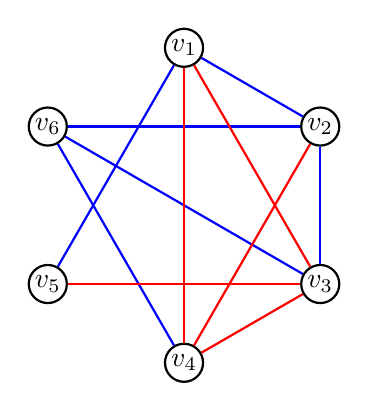
\begin{tikzpicture}
			\tikzset{punkt/.style={circle, thick, draw=black, minimum width=0.2cm,inner sep=1}}
			\node[punkt] at (0.0, 2.0) (a) {$v_1$};
			\node[punkt] at (1.73, 1.0) (b) {$v_2$};
			\node[punkt] at (1.73, -1.0) (c) {$v_3$};
			\node[punkt] at (0.0, -2.0) (d) {$v_4$};
			\node[punkt] at (-1.73, -1.0) (e) {$v_5$};
			\node[punkt] at (-1.73, 1.0) (f) {$v_6$};
			%\draw (0,0) circle [radius=2];

			% Blue edges
			\draw [thick, draw=blue] (a) -- (b);
			\draw [thick, draw=blue] (b) -- (c);
			\draw [thick, draw=blue] (e) -- (a);
			\draw [thick, draw=blue] (f) -- (d);
			\draw [thick, draw=blue] (f) -- (b);
			\draw [thick, draw=blue] (f) -- (c);

			% Red edges
			\draw [thick, draw=red] (a) -- (c);
			\draw [thick, draw=red] (c) -- (d);
			\draw [thick, draw=red] (b) -- (d);
			\draw [thick, draw=red] (c) -- (e);
			\draw [thick, draw=red] (a) -- (d);
		\end{tikzpicture}
		\caption{A graph $G$ with a $2$-edge coloring}
		\label{fig:cliques_and_neighbours}
	\end{figure}
	We see that $\mathcal{C}(G; 3) = \left\{G|_{\{v_1, v_2, v_3\}}, G|_{\{v_2, v_3, v_{6}\}}\right\}$ additionally we see that $\mathcal{N}(v_3; red) = \left\{v_1, v_{4}, v_5\right\}$ and $\mathcal{N}(v_3; blue) = \left\{v_2, v_{6}\right\}$.
\end{example}

\section{Existence of Ramsey Numbers}
This section is based upon \cite{rt}[Section 1.1].
\begin{definition}
	Let $\ell_1, \ell_2, \ldots, \ell_r, n \in \mathbb{N}^{+}$ we will write $n \to (\ell_1, \ell_2, \ldots, \ell_{r})$ if for every $r$-edge coloring $\chi: E(K_{n}) \to \left\{c_1, c_2, \ldots, c_{r}\right\}$ on $K_n$, there exists an $i \in \left\{1, 2, \ldots, r\right\}$ such that $\chi$ admits a $c_{i}$-monochromatic clique of order $\ell_{i}$.
\end{definition}
\begin{remark}
	Clearly $\ell_i \geq \ell_i'$ and $n \to (\ell_1, \ell_2, \ldots, \ell_{r})$ implies that $n \to (\ell_1', \ell_2', \ldots, \ell_{r}')$, since given an $r$-edge coloring $\chi: E(K_{n}) \to \left\{c_1, c_2, \ldots, c_{r}\right\}$ on $K_{n}$ there exists an $i \in [r]$ such that $K_n$ has a $c_{r}$-monochromatic clique of order $\ell_{i} \geq \ell_{i}'$.
\end{remark}

\begin{theorem}[Ramsey's Theorem]\label{thm:ramsey_two_colors}
	Let $\ell_1, \ell_2 \geq 2$, then there exists a $n \in \mathbb{N}^{+}$ such that $n \to (\ell_1, \ell_2)$.
\end{theorem}
\begin{proof}
	Clearly $\ell_1 \to (\ell_1, 2)$ and $\ell_2 \to (2, \ell_2)$ (after all either $K_{\ell_{i}}$ is monochromatic or there exist a monochromatic clique of order $2$). We will proceed using induction on $\ell_1 + \ell_{2}$, hence we may assume that $\ell_1 + \ell_2 \geq 6$, with $\ell_1, \ell_2 \geq 3$.
	Additionally by our induction hypothesis we may assume the existence of non-zero $n_1, n_2 \in \mathbb{N}$ such that $n_1 \to (\ell_1, \ell_2 - 1)$ and $n_2 \to (\ell_1 - 1, \ell_2)$. Next let $n := n_1 + n_2$ we will show that $n \to (\ell_1, \ell_2)$. Fix an arbitrary $2$-edge coloring $\chi: E(K_{n}) \to \left\{red, blue\right\}$ on $K_n$ and let $v$ be a vertex in $K_n$, then $v$ is adjacent to $n - 1$ other vertices in $K_{n}$, hence:
	\begin{equation*}
		n_1 + n_2 - 1 = n - 1 = \abs{\mathcal{N}_{\chi}(v; red)} + \abs{\mathcal{N}_{\chi}(v; blue)}
	\end{equation*}
	meaning either $\abs{N_{\chi}(v; red)} \geq n_2$ or $\abs{N_{\chi}(v; blue)} \geq n_1$, by the Generalized Pigeonhole Principle (Theorem \ref{thm:gpp}). Without loss of generality assume that the second inequality holds, namely $\abs{N_{\chi}(v; blue)} \geq n_1$. By our inductive hypothesis, the complete graph:
	\begin{equation*}
		G = \left(N_{\chi}(v; blue), E(K_{n}) \cap (N_{\chi}(v; blue) \times N_{\chi}(v; blue))\right)
	\end{equation*}
	contains either a $red$-monochromatic clique of order $\ell_{1}$ (in which case we are done) or a $blue$-monochromatic clique of order $\ell_{2} - 1$, in which case we note that $v$ is connected to the vertices in $N_{\chi}(v; 2)$ via edges which $\chi$ colors $blue$, and hence $K_n |_{\mathcal{N}_{\chi}(v, blue) \cup \left\{v\right\}}$ is a $blue$-monochromatic clique of order $\ell_{2}$.
\end{proof}

\begin{corollary}\label{cor:ramsey_for_arbitarily_many_colors}
	Let $\ell_1, \ell_2, \ldots, \ell_r \geq 2$, then there exists a $n \in \mathbb{N}^{+}$ such that $n \to (\ell_1, \ell_2, \ldots, \ell_{r})$.
\end{corollary}

\begin{proof}
	We proceed using induction on $r$, the base case $r = 2$ is proven in Theorem \ref{thm:ramsey_two_colors}.
	Next assume that the theorem holds for $r - 1$. From Theorem \ref{thm:ramsey_two_colors}, it follows that there exists a $\ell \in \mathbb{N}^{+}$ such that $\ell \to (\ell_{r - 1}, \ell_{r})$.
	By our induction hypothesis we may find a $n \in \mathbb{N}^{+}$ for which it holds that:
	\begin{equation*}
		n \to (\ell_1, \ell_2, \ldots, \ell_{r - 2}, \ell)
	\end{equation*}
	Now given any $r$-edge coloring $\chi: E(K_n) \to \left\{c_1, c_2, \ldots, c_{r}\right\}$ on $K_n$ we may obtain a $r - 1$-edge coloring $\chi': E(K_{n}) \to \left\{c_1, c_2, \ldots, c_{r-1}\right\}$ on $K_n$ by defining:
	\begin{equation*}
		\chi'(e) = \begin{cases} \chi(e) & \text{ if } \chi(e) \neq c_{r} \\ c_{r - 1} & \text{ if } \chi(e) = c_{r} \end{cases}
	\end{equation*}
	Hence $\chi'$ must either admit a $c_{i}$-monochromatic clique of order $\ell_i$, for some $i \in \left\{1, 2, \ldots, r - 2\right\}$ (in which case we are done) or a $c_{r - 1}$-monochromatic clique of order $\ell$. If the second case holds let $C$ be this $c_{r-1}$-monochromatic clique of order $\ell$, then $\chi$ colors every edge in $C$ with either $c_{r - 1}$ or $c_{r}$. However $\ell$ was chosen so that $\ell \to (\ell_{r - 1}, \ell_r)$, hence $C$ must contain either a $c_{r - 1}$-monochromatic clique of order $\ell_{r - 1}$ or a $c_{r}$-monochromatic clique of order $\ell_{r}$.
\end{proof}

\begin{definition}
	Let $\ell_1, \ell_2, \ldots, \ell_r \in \mathbb{N}^{+}$ the \textit{Ramsey number} $R(\ell_1, \ell_2, \ldots, \ell_{r})$, is the minimal $n \in \mathbb{N}^{+}$ such that $n \to (\ell_1, \ell_2, \ldots, \ell_{r})$, additionally we let $R(\ell; r)$ denote $R(\ell_1, \ell_2, \ldots, \ell_{r})$, with $\ell_1 = \ell_2 = \cdots = \ell_r = \ell$. The Ramsey numbers of the form $R(\ell; 2)$ are called \textit{digaonal Ramsey numbers}.
\end{definition}
\begin{remark}
	The Ramsey number $R(\ell,k)$ can also be thought of as the minimum order an arbitrary graph $G = (V, E)$ must be, to guarantee the existence of a clique of order $\ell$ or a set of $k$ independent vertices, that is there exists a set $U$ of $k$ verticies such that no two verticies in $U$ are adjacent.
\end{remark}
Generally direct computation of Ramsey numbers are extremely difficult, however there is some exceptions, for instance we have $R(2, \ell) = R(\ell, 2) = \ell$, confer the basis step in the proof of Theorem \ref{thm:ramsey_two_colors}, below we present another example.

\begin{example}\label{exmp:R3_3}
	In this example we will show that $R(3, 3) = 6$, we start by showing that $R(3, 3) \leq 6$. Consider an arbitary $2$-edge coloring $\chi: E(K_{6}) \to \left\{red, blue\right\}$ on $K_6$ and let $v$ be a vertex in $K_6$, then $v$ has $5$ adjacent neighbours, by the generalized pigeonhole principle, Theorem \ref{thm:gpp}, there is a color $c$ (either $red$ or $blue$) such that $\abs{\mathcal{N}_{\chi}(v; c)} \geq 3$.

	Without loss of generality we may assume that $c = red$. Next take pairwise distinct $v_1, v_2, v_3 \in \mathcal{N}_{\chi}(v; red)$, then we must have $\chi(v_{i}, v_{j}) = blue$ for pairwise distinct $i, j \in [3]$, otherwise $K_{6} |_{\left\{v, v_i, v_j\right\}}$ would form a $red$-monochromatic clique of order $3$. However this in turn means that $\chi(v_i, v_j) = blue$ for all pairwise distinct $i, j \in [3]$, hence $K_6 |_{\left\{v_1, v_2, v_3\right\}}$ forms a $blue$-monochromatic clique of order $3$.

	On the other hand it is easy to construct a $2$-edge coloring on $K_5$ which admit no monochromatic subclique of order $3$, one example of such a $2$-edge coloring is illustrated in Figure \ref{fig:K5_counter_example}.
	\begin{figure}[H]
		\centering
		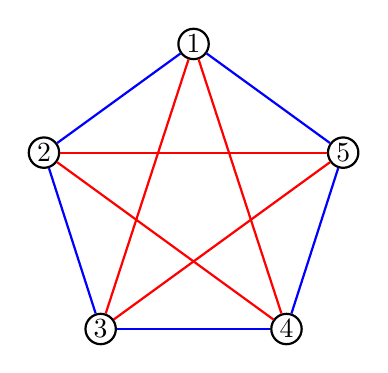
\begin{tikzpicture}
			\tikzset{punkt/.style={circle, thick, draw=black, minimum width=0.2cm,inner sep=1}}
			\node[punkt] at (0.0, 2.0) (a) {$1$};
			\node[punkt] at (-1.9, 0.62) (b) {$2$};
			\node[punkt] at (-1.18, -1.62) (c) {$3$};
			\node[punkt] at (1.18, -1.62) (d) {$4$};
			\node[punkt] at (1.9, 0.62) (e) {$5$};
			%\draw (0,0) circle [radius=2];

			% Blue edges
			\draw [thick, draw=blue] (a) -- (b);
			\draw [thick, draw=blue] (b) -- (c);
			\draw [thick, draw=blue] (c) -- (d);
			\draw [thick, draw=blue] (d) -- (e);
			\draw [thick, draw=blue] (e) -- (a);

			% Red edges
			\draw [thick, draw=red] (a) -- (c);
			\draw [thick, draw=red] (a) -- (d);
			\draw [thick, draw=red] (b) -- (d);
			\draw [thick, draw=red] (b) -- (e);
			\draw [thick, draw=red] (c) -- (e);
		\end{tikzpicture}
		\caption{A 2-edge coloring on $K_{5}$ that admits no monochromatic subclique of order $3$.}
		\label{fig:K5_counter_example}
	\end{figure}
	Finally since $R(3, 3) > 5$ and $R(3, 3) \leq 6$, we obtain that $R(3, 3) = 6$.
\end{example}
\newpage

We might also be interested in when an $r$-edge coloring of a complete graph admits some special monochromatic subgraphs, following this spirit we introduce the following definition:
\begin{definition}
	Let $G_1, G_2, \ldots, G_r$ be graphs, the \textit{generalized Ramsey number} $R(G_1, G_2, \ldots, G_{r})$ is the smallest integer $N$ such that for any $r$-edge coloring $\chi: E(K_N) \to \{c_1, c_2, \ldots, c_{r}\}$ there exists some index $i \in [1; r]$ such that there exists a $c_i$ monochromatic subgraph of $K_n$ which is isomorphic to $G_{i}$.
\end{definition}

It is worth noting that the generalized Ramsey number $R(G_1, G_2, \ldots, G_{r})$ is well defined. This can be seen as follows: let $\ell_j = \abs{V(G_{j})}$ consider the arbitrary $r$-coloring $\chi: E(K_n) \to \{c_1, c_2, \ldots, c_{r}\}$ of $K_n$ with $n = R(\ell_1, \ell_2, \ldots, \ell_{r})$. Then by the definition of $R(\ell_1, \ell_2, \ldots, \ell_{r})$ there exists an $i \in [1; r]$ such that $\chi$ admits a $c_i$-monochromatic clique of order $\ell_i$. The rest follows by the well ordering principle and the fact that $G_i$ is isomorphic to a subgraph of the previously mentioned $c_{i}$-monochromatic clique.

\section{Upper Bounds}\label{sec:upper_bound}
In this section we will prove several upper bounds for both regular and generalized Ramsey numbers, we will start by proving the following upper bound for $R(G_1, G_2, \ldots, G_{r})$.
\begin{theorem}\label{thm:ramsey_upper_bound}
	Let $G_1, G_2, \ldots, G_r$ be graphs with at least $2$ vertices, then:
	\begin{equation*}
		R(G_{1}, G_2, \ldots, G_{r}) \leq 2 - r + \sum_{i = 1}^r R(G_1, \ldots, G_{i - 1}, G_{i}', G_{i + 1}, \ldots, G_{r})
	\end{equation*}
	where the graph $G'$ is obtained from $G$ by deleting one vertex and all of the edges incident to it.
\end{theorem}
\begin{proof}
	For the sake of convenience we will let $R_i = R(G_1, \ldots, G_{i - 1}, G'_{i}, G_{i + 1}, \ldots, G_{r})$ throughout the proof.
	Let $N := 2 - r + \sum_{i = 1}^r R_{i}$ and $\chi$ be an $r$-edge coloring of $K_N$.
	Let $v \in V(K_{N})$, then $v$ is adjacent with $N - 1 = 1 +\sum_{i = 1}^r \left(R_{i} - 1\right)$ other vertices in $K_N$.
	By the Generalized Pigeon Hole Principle (Theorem \ref{thm:gpp}) there exists an $i \in [1; r]$ such that $\abs{\mathcal{N}_{\chi}(v, c_i)} \geq R_{i}$.
	By the definition of $R_i$, we have two cases:
	\begin{enumerate}
		\item Either $\chi$ admits a $c_j$-monochromatic subgraph which is isomorphic with $G_j$, with vertices belonging to $\mathcal{N}_{\chi}(v, c_{i})$, with $j \neq i$, in which case we are done.
		\item Or $\chi$ admits a $c_i$-monochromatic subgraph which is isomorphic with $G'_{i}$ with vertices belonging to $\mathcal{N}_{\chi}(v, c_i)$, of order $\ell_i - 1$, in which case adding $v$ along with the appropriate edges in the set $\left\{\{v, u\} \middle| u \in \mathcal{N}_{\chi}(v, c_{i})\right\}$ forms a $c_i$-monochromatic subgraph which is isomorphic with $G_{i}$. \qedhere
	\end{enumerate}
\end{proof}

In particular Theorem \ref{thm:ramsey_upper_bound}, with $G_i = K_{\ell_{i}}$ implies that:
\begin{equation}\label{eq:cor_1}
	R \left(\ell_1, \ell_2, \ldots, \ell_{r}\right) \leq 2 - r +  \sum_{i = 1}^r R(\ell_1, \ldots, \ell_{i - 1}, \ell_i, \ell_{i + 1}, \ldots, \ell_{r})
\end{equation}

\newpage
\begin{corollary}\label{cor:R3r}
	Let $r \in \mathbb{N}^{+}$ then $R(3; r) \leq 3r!$.
\end{corollary}
\begin{proof}
	We will prove the corollary using induction on $r$. Clearly the result holds in the case where $r = 1$. Next for an arbitrary $r \in \mathbb{N}^{+}$ it follows by Equation \eqref{eq:cor_1}, that:
	\begin{equation}\label{eq:R3r}
		R(3; r) \stackrel{(a)}{\leq} r R(2, 3, \ldots, 3) \stackrel{(b)}{=} r R(3; r - 1) \stackrel{(c)}{=} 3r (r - 1)! = 3r!
	\end{equation}
	where $(a)$ follows by Equation \eqref{eq:R3r}, $(b)$ follows since letting $n := R(2, 3, \ldots, 3)$ we see that every $r$-edge coloring on $K_n$ either admits a monochromatic clique of order $2$ of the appropriate color or we actually have $(r - 1)$-edge coloring on $K_n$. Finally $(c)$ follows directly by the induction hypothesis.
\end{proof}


%\begin{proposition}\label{prop:upper_bounds_form_ramseys_theorem}
%	Let $G, H$ be graphs with $\abs{V(G)}, \abs{V(H)} \geq 2$ and let $G'$ and $H'$ be subgraphs of $G$ and $H$ respectively obtained by deleting a vertex and the appropriate edges, then:
%	\begin{equation*}
%		R(G, H) \leq R(G', H) + R(G, H')
%	\end{equation*}
%\end{proposition}
%We will omit the proof, but note that the basic argument is the same as in the proof of Theorem \ref{thm:ramsey_two_colors}.
The following Corollary is a natural consequence of Theorem \ref{thm:ramsey_upper_bound} and the fact that $R(\ell, 2) = R(2, \ell) = \ell$ for all $\ell \geq 2$.
\begin{corollary}
	Let $\ell, k \in \mathbb{N}$ with $\ell, k \geq 2$, then $R(\ell, k) \leq \binom{\ell + k - 2}{\ell - 1}$
\end{corollary}
\begin{proof}
	We will apply induction on $\ell + k$, in the case where $\ell = 2$ we get that
	\begin{equation*}
		R(\ell, k) = k = \frac{k!}{(k - 1)!} = \binom{k + \ell - 2}{\ell - 1}
	\end{equation*}
	The case where $k = 2$ follows in a similar manner. Next we assume that $\ell, k \geq 3$, then:
	\begin{align*}
		R(\ell, k) \stackrel{(a)}{\leq} R(\ell - 1, k) + R(\ell, k - 1) & \stackrel{(b)}{\leq} \binom{(\ell - 1) + k - 2}{(\ell - 1) - 1} + \binom{\ell + (k - 1) - 2}{\ell - 1} \\
		                                                                & =  \frac{(\ell + k - 3)!}{(\ell - 2)!(k - 1)!} + \frac{(\ell + k - 3)!}{(\ell - 1)!(k - 2)!}           \\
		                                                                & =  \frac{(\ell + k - 3)!((\ell - 1) + (k - 1))}{(\ell - 1)!(k - 1)!}
		= \binom{\ell + k - 2}{\ell - 1}
	\end{align*}
	Where $(a)$ follows by Equation \eqref{eq:cor_1} and $(b)$ directly from the induction hypothesis.
\end{proof}

\begin{corollary}\label{cor:upper_bounds_from_ramseys_theorem_even}
	Let $G, H$ be graphs with at least two edges and let $G'$ and $H'$ be subgraphs of $G$ and $H$ respectively obtained by deleting a vertex and the appropriate edges, then if both $R(G', H)$ and $R(G, H')$ are even, then:
	\begin{equation*}
		R(G, H) \leq R(G', H) + R(G, H') - 1
	\end{equation*}
\end{corollary}
\begin{proof}
	Assume for the sake of contradiction that the inequality does not hold, then by Theorem \ref{thm:ramsey_upper_bound}, we must have $N := R(G, H) = R(G', H) + R(G, H')$ and hence there exists an $2$-edge coloring $\chi: E(K_{N - 1}) \to \left\{red, blue\right\}$ of $K_{N - 1}$ which admits no $red$-monochromatic subgraphs which are isomorphic to $G$ and no $blue$-monochromatic subgraph which are isomorphic to $H$. For all $v \in V(K_{N - 1})$ we thus must have:
	\begin{equation*}
		\abs{\mathcal{N}_{\chi}(v; red)} \leq R(G', H) - 1 \text{ and } \abs{\mathcal{N}_{\chi}(v; blue)} \leq R(G, H') - 1
	\end{equation*}
	since we would otherwise have a $red$(or $blue$)-monochromatic subgraph which is isomorphic to $G$ (or $H$). Next since $v$ is adjacent to $N - 2 = R(G', H) + R(G, H') - 2$ vertices we see that we must have:
	\begin{equation*}
		\abs{\mathcal{N}_{\chi}(v; red)} = R(G', H) - 1 \text{ and } \abs{\mathcal{N}_{\chi}(v; blue)} = R(G, H') - 1
	\end{equation*}
	Next let $k := \abs{\left\{e \in E(K_{N - 1}) | \chi(e) = red\right\}}$ that is $k$ is the number of edges which $\chi$, colors $red$. Thus we may also compute $k$ as:
	\begin{equation}\label{eq:k_is_not_integer}
		k = \frac{1}{2}\sum_{u \in V(K_{N - 1})}\abs{\mathcal{N}_{\chi}(u; red)} = \frac{1}{2}(N - 1)(R(G', H) - 1)
	\end{equation}
	however both $N-1$ and $R(G', H) - 1$ are odd by our assumptions, combining this with Equation \eqref{eq:k_is_not_integer}, implies that $k$ is not natural number a clear contradiction.
\end{proof}

\section{Lower Bounds and the Probabilistic Method}\label{sec:lower_bound}
The probabilistic methodprobability was pioneered by Paul Erdős, and it is generally used throughout combinatorics to establish various lower bounds using methods from probability theory, for graph Ramsey theory it yields some of the best lowerbounds for large Ramsey numbers. Suppose we wish to find a lower bound for $R(\ell_1, \ell_2, \ldots,  \ell_{r})$ the basic idea, at least when applying the method to graph Ramsey theory is to consider a random $r$-edge coloring $\chi$ on a the complete graph $K_{N}$. If the probability, that there exists no indices $i \in [1; r]$ such that $\chi$ admits a $c_{i}$-monochromatic clique of order $\ell_{i}$, is less than $1$, then we must have:
\begin{equation*}
	R(\ell_1, \ell_2, \ldots, \ell_{r}) > N
\end{equation*}
We will need the following lemma, which we state without proof.

\begin{lemma}[Stirlings formula]\label{lem:stirling}
	Let $n \in \mathbb{N}$, then:
	\begin{equation*}
		n! > \sqrt{2 \pi n} \left(\frac{n}{\e}\right)^{n}
	\end{equation*}
\end{lemma}
We now state and prove the main theorem of this section.
\begin{theorem}
	Let $r, \ell \geq 2$, then:
	\begin{equation*}
		R(\ell; r) > \frac{\left(2\pi \ell\right)^{\frac{1}{2\ell}}\ell \sqrt{r}^{\ell}}{r^{\frac{1}{2\ell}}\e}
	\end{equation*}
\end{theorem}
\begin{proof}
	Let $N \geq \ell$ be arbitrary for now. Let $\chi: E(K_N) \to \left\{c_1, c_2, \ldots, c_{r}\right\}$ be a random $r$-edge coloring, with each edge $e$ colored uniformly and independently of the other edges, that is $\mathbb{P}(\chi(e) = c_{i}) = \frac{1}{r}$ for every $i \in [1; r]$. Enumerate the $\ell$-cliques of $K_{N}$ as $C_1, C_2, \ldots, C_{\binom{N}{\ell}}$ and consider the stochastic variables $X_1, X_2, \ldots X_{\binom{N}{\ell}}$ as:
	\begin{equation*}
		X_i = \begin{cases}
			1 & \text{ if } \abs{\chi(E(G \vert_{C_i}))} = 1 \\
			0 & \text{ otherwise }
		\end{cases}
	\end{equation*}
	that is $X_i$ is an indicator function which indicates if the clique $C_i$ is monochromatic under $\chi$. Next notice that
	\begin{equation}\label{eq:prop_mon_clique}
		\mathbb{P}(X_i = 1) = r \cdot \left(\frac{1}{r}\right)^{\binom{\ell}{2}} = r \cdot \left(\frac{\sqrt{r}}{\sqrt{r}^{\ell}}\right)^\ell
	\end{equation}
	since $\abs{E(G \vert_{C_i})} = \binom{\ell}{2} = \frac{\ell^2 - \ell}{2}$. Thus:
	\begin{equation}\label{eq:prob_method}
		\mathbb{E} \left[\sum_{i = 1}^{\binom{N}{\ell}} X_{i}\right]
		= \sum_{i = 1}^{\binom{N}{\ell}} \mathbb{P}(X_i = 1)
		\stackrel{(a)}{\leq} \frac{N^{\ell}}{\ell!} \frac{r}{r^{\binom{\ell}{2}}}
		\stackrel{(b)}{<} \frac{N^{\ell}r}{\sqrt{2\pi \ell} \left(\frac{\ell}{\e}\right)^{\ell}}   \left(\frac{\sqrt{r}}{\sqrt{r}^{\ell}}\right)^{\ell}
		= \frac{r}{\sqrt{2\pi\ell}} \left(\frac{N \e \sqrt{r}}{\ell \sqrt{r}^{\ell}}\right)^{\ell}
	\end{equation}
	where $(a)$ follows by Equation \eqref{eq:prop_mon_clique} and $\frac{N!}{(N - \ell)!} = \prod^N_{k = N - \ell + 1} k < N^{\ell}$ and $(b)$ by Stirlings formula (Lemma \ref{lem:stirling}). \\
	The rest follows as $\frac{r}{\sqrt{2\pi\ell}} \left(\frac{N \e \sqrt{r}}{\ell \sqrt{r}^{\ell}}\right)^{\ell} \geq 1$ if and only if $N \geq \frac{\ell \sqrt{r}^{\ell}}{\e \sqrt{r}} \left(\frac{\sqrt{2\pi\ell}}{r}\right)^{\frac{1}{\ell}}$. Thus since inequality $(b)$ is strict we see that $R(\ell; r) > \frac{\ell \sqrt{r}^{\ell}}{\e \sqrt{r}} \left(\frac{\sqrt{2\pi\ell}}{r}\right)^{\frac{1}{\ell}}$.
	%Now if $\frac{r}{\sqrt{2\pi\ell}} \leq 1$, then setting $N := \frac{\ell\sqrt{r}^{\ell}}{e \sqrt{r}}$ implies $\mathbb{E} \left[\sum_{i = 1}^{\binom{N}{\ell}} X_{i}\right] < 1$, by Equation \eqref{eq:prob_method}, meaning $R(\ell; r) > N$. Alternately if $\frac{r}{\sqrt{2\pi\ell}}$ setting $N := \frac{\ell \sqrt{r}^{\ell}}{\e \sqrt{r}} \left(\frac{\sqrt{2\pi\ell}}{r}\right)^{\frac{1}{\ell}}$, then Equation \eqref{eq:prob_method}, once again gives $\mathbb{E} \left[\sum_{i = 1}^{\binom{N}{\ell}} X_{i}\right] < 1$ concluding the proof.
\end{proof}
%\begin{theorem}
%	Let $\ell \geq 3$ then $R(\ell, \ell) > \frac{\ell}{\e \sqrt{2}} 2^{\ell / 2}$.
%\end{theorem}
%\begin{proof}
%	Let $\chi: E(K_N) \to \left\{red, blue\right\}$ be a random $2$-edge coloring with, we will assume the $\chi(e)$ of is chosen uniformly and independently. Let $C$ be a subgraph of $K_N$ such that $C$ forms a clique and $A_C$ be the event that $\abs{\chi(E(G \vert_{C}))} = 1$, meaning $C$ is monochromatic. Then:
%	\begin{equation*}
%		\mathbb{P}(A_C) = 2 \left(\frac{1}{2} \right)^{\binom{\ell}{2}} = 2^{1 - \binom{\ell}{2}}
%	\end{equation*}
%	since all $\binom{\ell}{2}$ edges of $C$ is must be colored the same color by $\chi$. Let $\mathcal{C}(K_N;\ell)$ be the set of cliques of $K_N$ of order $\ell$, then:
%	\begin{equation*}
%		\mathbb{P} \left(\bigcup_{C \in \mathcal{C}(K_{N}; \ell)} A_{C}\right) \leq \sum_{C \in \mathcal{C}(K_N; \ell)} \mathbb{P}(A_{C}) = \binom{N}{\ell} 2^{1 - \binom{\ell}{2}}
%	\end{equation*}
%	which follows as $\mathcal{C}(K_N; \ell) = \binom{N}{\ell}$. Now if this probability is strictly less than $1$, we must have:
%	\begin{equation*}
%		\mathbb{P}\left(\bigcap_{C \in \mathcal{C}(K_N; \ell)} \overline{A_{C}}\right) = 1 - \mathbb{P} \left(\bigcup_{C \in \mathcal{C}(K_{N}; \ell)} A_{C}\right) \neq 0
%	\end{equation*}
%	where $\overline{A_C}$ is the complement of $A_C$, meaning it is the event that $C$ is not a monochromatic clique. Meaning if this is the case then there must exist a $2$-edge coloring which emits no monochromatic clique of order $\ell$. However it remains to find an integer $N$ such that $\mathbb{P} \left(\bigcup_{C \in \mathcal{C}(K_{N}; \ell)} A_{C}\right) < 1$. We start by computing an upper bound, for the probability that there is at least one monochromatic clique in $K_N$:
%	\begin{equation*}
%		\mathbb{P} \left(\bigcup_{C \in \mathcal{C}(K_{N}; \ell)} A_{C}\right) \leq \binom{N}{\ell} 2^{1 - \binom{\ell}{2}} \stackrel{(a)}{\leq} \frac{N^{\ell}}{\ell!} 2^{1 - \binom{\ell}{2}} \stackrel{(b)}{<} \frac{2}{\sqrt{2\pi \ell}} \left(\frac{\e \sqrt{2} N}{\ell 2^{\ell/2}}\right)^{\ell}
%	\end{equation*}
%	where inequality $(a)$ follow as $\binom{N}{\ell} = \frac{N(N - 1)\cdots(N - \ell + 1)}{\ell!} \leq \frac{N^{\ell}}{\ell!}$ and $(b)$ by Stirlings formula (Lemma \ref{lem:stirling}) and the fact that:
%	\begin{equation*}
%		2^{1 - \binom{\ell}{2}} = 2 \cdot 2^{(-\ell^2 + \ell) / 2} = \frac{2 \cdot \sqrt{2}^{\ell}}{2^{\frac{\ell^2}{2}}}
%	\end{equation*}
%	The rest follows by setting $N = \frac{\ell}{\e \sqrt{2}} 2^{\ell / 2}$.
%\end{proof}

The following theorem are based upon \cite{fg_and_rt}[Theorem 5.5] and gives us our first lower bound for the non-diagonal Ramsey numbers, note that the theorem can also be applied recursively to give a lower bound a general Ramsey number $R(\ell_1, \ell_2, \ldots, \ell_{r})$, via a process similar to the approach used in the proof of Corollary \ref{cor:ramsey_for_arbitarily_many_colors}.
\begin{theorem}
	Let $\ell \geq 2$, there exists a $c_{\ell} > 0$ such that:
	\begin{equation*}
		R(\ell, k) \geq c_{\ell} \left(\frac{k}{\log(k)}\right)^{\frac{\ell - 1}{2}}
	\end{equation*}
	for all $k \geq 2$.
\end{theorem}
We will only give a sketch of the proof.
\begin{proof}[Proof (Sketch)]
	Let $N = \floor{c_{\ell} \left(\frac{k}{\log(k)}\right)^{\frac{\ell - 1}{2}}}$\footnote{Please note that $N$, is not actually fixed, but rahter $N$ depends on $c_{\ell}$.} and $\chi: E(K_N) \to \left\{red, blue\right\}$ be a random $2$-edge coloring on $K_N$, with each edge $e \in E(K_{N})$ colored independently of the others, and with $\mathbb{P}(\chi(e) = red) = \frac{1}{N^{\frac{2}{\ell  - 1}}}$. Next enumerate the $\ell$ and $k$ cliques of $K_N$ as $C_1, C_2, \ldots, C_{\binom{N}{\ell}}$ and $C'_1, C'_2, \ldots, C'_{\binom{N}{k}}$ respectively. We will define the stochastic variables $X_1, X_2, \ldots, X_{\binom{N}{\ell}}$ and $Y_1, Y_2, \ldots, Y_{\binom{N}{k}}$ as:
	\begin{equation*}
		X_i = \begin{cases}
			1 & \text{ if } \chi(E(G \vert_{C_i})) = \left\{red\right\} \\
			0 & \text{ otherwise }
		\end{cases}
	\end{equation*}
	and
	\begin{equation*}
		Y_i = \begin{cases}
			1 & \text{ if } \chi(E(G \vert_{C'_i})) = \left\{blue\right\} \\
			0 & \text{ otherwise }
		\end{cases}
	\end{equation*}
	Letting $p := \mathbb{P}(\chi(e) = red)$ we see that:
	\begin{equation*}
		\mathbb{E} \left[\sum_{i = 1}^{\binom{N}{\ell}} X_i + \sum_{i = 1}^{\binom{N}{k}} Y_{i}\right] \stackrel{a}{=} \binom{N}{\ell} p^{\binom{\ell}{2}} + \binom{N}{k}(1 - p)^{\binom{k}{2}}
	\end{equation*}
	where $(a)$ follows since each edge is colored independently meaning $\mathbb{P} \left(X_i = 1\right) = p^{\binom{\ell}{2}}$ since each of the $\binom{\ell}{2}$ edges in $G \vert_{C_i}$ must be colored $red$ by $\chi$ and similarly $Y_j = 1$ if and only if each edge in $G \vert_{C'_{i}}$ is colored $blue$ by $\chi$. Finally we note that if $c_{\ell}$ is chosen sufficiently small, then $\binom{N}{\ell} p^{\binom{\ell}{2}} + \binom{N}{k}(1 - p)^{\binom{k}{2}} < 1$.
\end{proof}

\section{Exact Values of Small Ramsey Numbers}\label{sec:exact_values}
In this section we compute the exact values of some of the smaller ramsey numbers, using some of the upper bounds which we proved in Section \ref{sec:upper_bound}. The section will be based upon \cite{emogrt}[Chapter 2].
\begin{theorem}\label{thm:small_ramsey_numbers}
	$R(3, 4) = 9, R(3, 5) = 14$ and $R(4, 4) = 18$.
\end{theorem}
\begin{proof}
	by Corollary \ref{cor:upper_bounds_from_ramseys_theorem_even}, we have:
	\begin{equation}\label{eq:R3_4}
		R(3, 4) \leq R(2, 4) + R(3, 3) - 1 = 9
	\end{equation}
	since $R(2, 4) = 4$ and $R(3, 3) = 6$ by Example \ref{exmp:R3_3}. More over by Theorem \ref{thm:ramsey_upper_bound} and Equation \eqref{eq:R3_4} we have:
	\begin{equation}\label{eq:R3_5}
		R(3, 5) \leq R(2, 5) + R(3, 4) \leq 5 + 9 = 14
	\end{equation}
	If we can construct a $2$-edge coloring $\chi: E(K^{*}_{13}) \to \left\{red, blue\right\}$ on $K^{*}_{13}$ with no $red$-clique of order $3$ and no $blue$ clique of order $5$, then we may conclude that $R(3, 5) = 14$ and hence $R(3, 4) = 9$ by Equations \eqref{eq:R3_4} and \eqref{eq:R3_5}. It is in fact the case that we may construct such a $2$-edge coloring $\chi$ on $K^{*}_{13}$ one example of such a coloring is:
	\begin{equation*}
		\chi(\{i, j\}) = \begin{cases}
			red  & \text{ if } [i - j]_{13} \in \left\{1, 5, 8, 12\right\} \\
			blue & \text{ otherwise }
		\end{cases}
	\end{equation*}
	Please note that $\chi$ is well defined since $-1 \equiv 12 \mod 13$ and $-5 \equiv 8 \mod 13$ and hence $[i - j]_{13} \in \left\{1, 5, 8, 12\right\}$ if and only if $[j - i]_{13} \in \left\{1, 5, 8, 12\right\}$. The fact that $\chi$ admits no $red$-monochromatic cliques of order $3$ and no $blue$-monochromatic cliques of order $5$ is checked via the code in Appendix \ref{app:ramsey_code}.
	Additionally since $R(3, 4) = 14$ we have $R(4, 4) \leq R(3, 4) + R(4, 3) = 18$, once again by Theorem \ref{thm:ramsey_upper_bound}, using this inequality we can show that $R(4, 4) = 18$ by constructing a $2$-edge coloring $\gamma: E(K^{*}_{17}) \to \left\{red, blue\right\}$ which admits no $red$ or $blue$ monochromatic cliques of order $4$. One such $2$-edge coloring is given below:
	\begin{equation*}
		\gamma(\left\{i, j\right\}) = \begin{cases}
			red  & \text{ if } [i -  j]_{17} \in \left\{1, 2, 4, 8, 9, 13, 15, 16\right\} \\
			blue & otherwise
		\end{cases}
	\end{equation*}
	again please note that $\gamma$ is well defined, just like $\chi$, by an identical argument. Again the fact that $\gamma$ admits no $red$ or $blue$ monochromatic cliques of order $5$ is checked via the code in Appendix \ref{app:ramsey_code}.
\end{proof}

For the sake of illustration $K^{*}_{13}$ equiped with the $2$-edge coloring $\chi$ and $K^{*}_{17}$ equiped with the $2$-edge coloring $\gamma$, both from the proof of Theorem \ref{thm:small_ramsey_numbers} is illustated below in Figures \ref{fig:small_ramsey_graphs}
\begin{figure}[H]
	\begin{subfigure}[c]{0.4\textwidth}
		\centering
		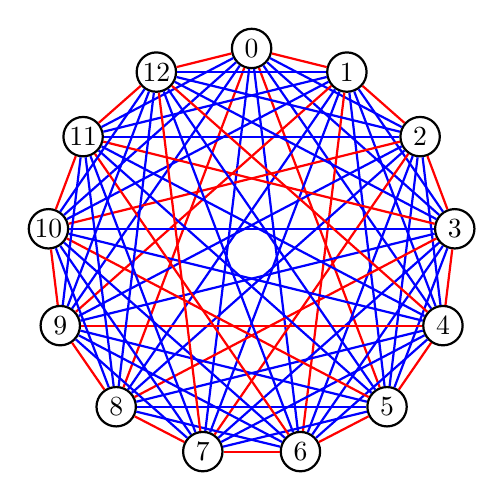
\begin{tikzpicture}
			\tikzset{punkt/.style={circle, thick, draw=black, minimum width=0.5cm,inner sep=0.2}}

			\node[punkt] at (0.0, 2.6) (a) {$0$};
			\node[punkt] at (1.21, 2.3) (b) {$1$};
			\node[punkt] at (2.14, 1.48) (c) {$2$};
			\node[punkt] at (2.58, 0.31) (d) {$3$};
			\node[punkt] at (2.43, -0.92) (e) {$4$};
			\node[punkt] at (1.72, -1.95) (f) {$5$};
			\node[punkt] at (0.62, -2.52) (g) {$6$};
			\node[punkt] at (-0.62, -2.52) (h) {$7$};
			\node[punkt] at (-1.72, -1.95) (i) {$8$};
			\node[punkt] at (-2.43, -0.92) (j) {$9$};
			\node[punkt] at (-2.58, 0.31) (k) {$10$};
			\node[punkt] at (-2.14, 1.48) (l) {$11$};
			\node[punkt] at (-1.21, 2.3) (m) {$12$};
			\draw [thick, draw=red] (a) -- (b);
			\draw [thick, draw=blue] (a) -- (c);
			\draw [thick, draw=blue] (a) -- (d);
			\draw [thick, draw=blue] (a) -- (e);
			\draw [thick, draw=red] (a) -- (f);
			\draw [thick, draw=blue] (a) -- (g);
			\draw [thick, draw=blue] (a) -- (h);
			\draw [thick, draw=red] (a) -- (i);
			\draw [thick, draw=blue] (a) -- (j);
			\draw [thick, draw=blue] (a) -- (k);
			\draw [thick, draw=blue] (a) -- (l);
			\draw [thick, draw=red] (a) -- (m);
			\draw [thick, draw=red] (b) -- (c);
			\draw [thick, draw=blue] (b) -- (d);
			\draw [thick, draw=blue] (b) -- (e);
			\draw [thick, draw=blue] (b) -- (f);
			\draw [thick, draw=red] (b) -- (g);
			\draw [thick, draw=blue] (b) -- (h);
			\draw [thick, draw=blue] (b) -- (i);
			\draw [thick, draw=red] (b) -- (j);
			\draw [thick, draw=blue] (b) -- (k);
			\draw [thick, draw=blue] (b) -- (l);
			\draw [thick, draw=blue] (b) -- (m);
			\draw [thick, draw=red] (c) -- (d);
			\draw [thick, draw=blue] (c) -- (e);
			\draw [thick, draw=blue] (c) -- (f);
			\draw [thick, draw=blue] (c) -- (g);
			\draw [thick, draw=red] (c) -- (h);
			\draw [thick, draw=blue] (c) -- (i);
			\draw [thick, draw=blue] (c) -- (j);
			\draw [thick, draw=red] (c) -- (k);
			\draw [thick, draw=blue] (c) -- (l);
			\draw [thick, draw=blue] (c) -- (m);
			\draw [thick, draw=red] (d) -- (e);
			\draw [thick, draw=blue] (d) -- (f);
			\draw [thick, draw=blue] (d) -- (g);
			\draw [thick, draw=blue] (d) -- (h);
			\draw [thick, draw=red] (d) -- (i);
			\draw [thick, draw=blue] (d) -- (j);
			\draw [thick, draw=blue] (d) -- (k);
			\draw [thick, draw=red] (d) -- (l);
			\draw [thick, draw=blue] (d) -- (m);
			\draw [thick, draw=red] (e) -- (f);
			\draw [thick, draw=blue] (e) -- (g);
			\draw [thick, draw=blue] (e) -- (h);
			\draw [thick, draw=blue] (e) -- (i);
			\draw [thick, draw=red] (e) -- (j);
			\draw [thick, draw=blue] (e) -- (k);
			\draw [thick, draw=blue] (e) -- (l);
			\draw [thick, draw=red] (e) -- (m);
			\draw [thick, draw=red] (f) -- (g);
			\draw [thick, draw=blue] (f) -- (h);
			\draw [thick, draw=blue] (f) -- (i);
			\draw [thick, draw=blue] (f) -- (j);
			\draw [thick, draw=red] (f) -- (k);
			\draw [thick, draw=blue] (f) -- (l);
			\draw [thick, draw=blue] (f) -- (m);
			\draw [thick, draw=red] (g) -- (h);
			\draw [thick, draw=blue] (g) -- (i);
			\draw [thick, draw=blue] (g) -- (j);
			\draw [thick, draw=blue] (g) -- (k);
			\draw [thick, draw=red] (g) -- (l);
			\draw [thick, draw=blue] (g) -- (m);
			\draw [thick, draw=red] (h) -- (i);
			\draw [thick, draw=blue] (h) -- (j);
			\draw [thick, draw=blue] (h) -- (k);
			\draw [thick, draw=blue] (h) -- (l);
			\draw [thick, draw=red] (h) -- (m);
			\draw [thick, draw=red] (i) -- (j);
			\draw [thick, draw=blue] (i) -- (k);
			\draw [thick, draw=blue] (i) -- (l);
			\draw [thick, draw=blue] (i) -- (m);
			\draw [thick, draw=red] (j) -- (k);
			\draw [thick, draw=blue] (j) -- (l);
			\draw [thick, draw=blue] (j) -- (m);
			\draw [thick, draw=red] (k) -- (l);
			\draw [thick, draw=blue] (k) -- (m);
			\draw [thick, draw=red] (l) -- (m);
		\end{tikzpicture}
		\caption{The $2$-edge coloring $\chi$ on $K^{*}_{13}$}
	\end{subfigure}
	\begin{subfigure}[c]{0.6\textwidth}
		\centering
		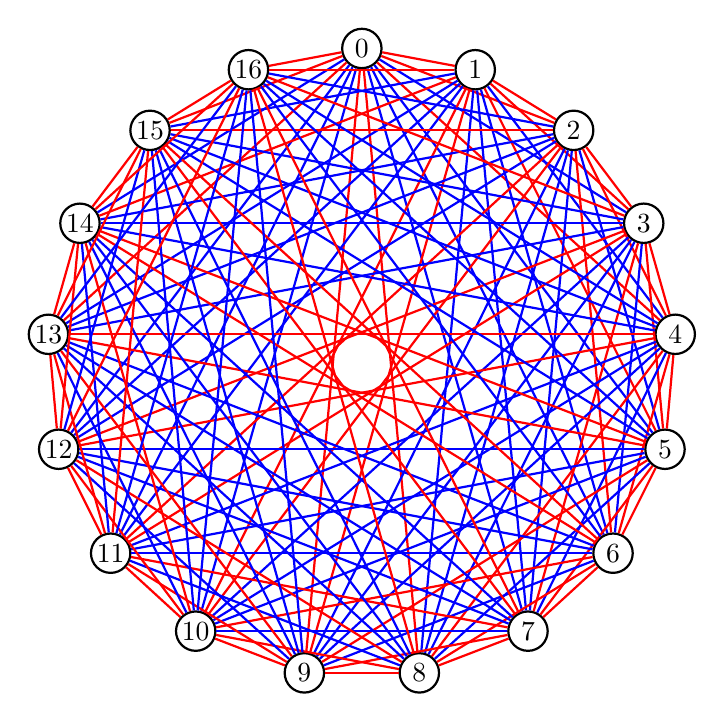
\begin{tikzpicture}
			\tikzset{punkt/.style={circle, thick, draw=black, minimum width=0.5cm,inner sep=0.2}}
			\node[punkt] at (0.0, 4.0) (a) {$0$};
			\node[punkt] at (1.44, 3.73) (b) {$1$};
			\node[punkt] at (2.69, 2.96) (c) {$2$};
			\node[punkt] at (3.58, 1.78) (d) {$3$};
			\node[punkt] at (3.98, 0.37) (e) {$4$};
			\node[punkt] at (3.85, -1.09) (f) {$5$};
			\node[punkt] at (3.19, -2.41) (g) {$6$};
			\node[punkt] at (2.11, -3.4) (h) {$7$};
			\node[punkt] at (0.73, -3.93) (i) {$8$};
			\node[punkt] at (-0.73, -3.93) (j) {$9$};
			\node[punkt] at (-2.11, -3.4) (k) {$10$};
			\node[punkt] at (-3.19, -2.41) (l) {$11$};
			\node[punkt] at (-3.85, -1.09) (m) {$12$};
			\node[punkt] at (-3.98, 0.37) (n) {$13$};
			\node[punkt] at (-3.58, 1.78) (o) {$14$};
			\node[punkt] at (-2.69, 2.96) (p) {$15$};
			\node[punkt] at (-1.44, 3.73) (q) {$16$};
			\draw [thick, draw=red] (a) -- (b);
			\draw [thick, draw=red] (a) -- (c);
			\draw [thick, draw=blue] (a) -- (d);
			\draw [thick, draw=red] (a) -- (e);
			\draw [thick, draw=blue] (a) -- (f);
			\draw [thick, draw=blue] (a) -- (g);
			\draw [thick, draw=blue] (a) -- (h);
			\draw [thick, draw=red] (a) -- (i);
			\draw [thick, draw=red] (a) -- (j);
			\draw [thick, draw=blue] (a) -- (k);
			\draw [thick, draw=blue] (a) -- (l);
			\draw [thick, draw=blue] (a) -- (m);
			\draw [thick, draw=red] (a) -- (n);
			\draw [thick, draw=blue] (a) -- (o);
			\draw [thick, draw=red] (a) -- (p);
			\draw [thick, draw=red] (a) -- (q);
			\draw [thick, draw=red] (b) -- (c);
			\draw [thick, draw=red] (b) -- (d);
			\draw [thick, draw=blue] (b) -- (e);
			\draw [thick, draw=red] (b) -- (f);
			\draw [thick, draw=blue] (b) -- (g);
			\draw [thick, draw=blue] (b) -- (h);
			\draw [thick, draw=blue] (b) -- (i);
			\draw [thick, draw=red] (b) -- (j);
			\draw [thick, draw=red] (b) -- (k);
			\draw [thick, draw=blue] (b) -- (l);
			\draw [thick, draw=blue] (b) -- (m);
			\draw [thick, draw=blue] (b) -- (n);
			\draw [thick, draw=red] (b) -- (o);
			\draw [thick, draw=blue] (b) -- (p);
			\draw [thick, draw=red] (b) -- (q);
			\draw [thick, draw=red] (c) -- (d);
			\draw [thick, draw=red] (c) -- (e);
			\draw [thick, draw=blue] (c) -- (f);
			\draw [thick, draw=red] (c) -- (g);
			\draw [thick, draw=blue] (c) -- (h);
			\draw [thick, draw=blue] (c) -- (i);
			\draw [thick, draw=blue] (c) -- (j);
			\draw [thick, draw=red] (c) -- (k);
			\draw [thick, draw=red] (c) -- (l);
			\draw [thick, draw=blue] (c) -- (m);
			\draw [thick, draw=blue] (c) -- (n);
			\draw [thick, draw=blue] (c) -- (o);
			\draw [thick, draw=red] (c) -- (p);
			\draw [thick, draw=blue] (c) -- (q);
			\draw [thick, draw=red] (d) -- (e);
			\draw [thick, draw=red] (d) -- (f);
			\draw [thick, draw=blue] (d) -- (g);
			\draw [thick, draw=red] (d) -- (h);
			\draw [thick, draw=blue] (d) -- (i);
			\draw [thick, draw=blue] (d) -- (j);
			\draw [thick, draw=blue] (d) -- (k);
			\draw [thick, draw=red] (d) -- (l);
			\draw [thick, draw=red] (d) -- (m);
			\draw [thick, draw=blue] (d) -- (n);
			\draw [thick, draw=blue] (d) -- (o);
			\draw [thick, draw=blue] (d) -- (p);
			\draw [thick, draw=red] (d) -- (q);
			\draw [thick, draw=red] (e) -- (f);
			\draw [thick, draw=red] (e) -- (g);
			\draw [thick, draw=blue] (e) -- (h);
			\draw [thick, draw=red] (e) -- (i);
			\draw [thick, draw=blue] (e) -- (j);
			\draw [thick, draw=blue] (e) -- (k);
			\draw [thick, draw=blue] (e) -- (l);
			\draw [thick, draw=red] (e) -- (m);
			\draw [thick, draw=red] (e) -- (n);
			\draw [thick, draw=blue] (e) -- (o);
			\draw [thick, draw=blue] (e) -- (p);
			\draw [thick, draw=blue] (e) -- (q);
			\draw [thick, draw=red] (f) -- (g);
			\draw [thick, draw=red] (f) -- (h);
			\draw [thick, draw=blue] (f) -- (i);
			\draw [thick, draw=red] (f) -- (j);
			\draw [thick, draw=blue] (f) -- (k);
			\draw [thick, draw=blue] (f) -- (l);
			\draw [thick, draw=blue] (f) -- (m);
			\draw [thick, draw=red] (f) -- (n);
			\draw [thick, draw=red] (f) -- (o);
			\draw [thick, draw=blue] (f) -- (p);
			\draw [thick, draw=blue] (f) -- (q);
			\draw [thick, draw=red] (g) -- (h);
			\draw [thick, draw=red] (g) -- (i);
			\draw [thick, draw=blue] (g) -- (j);
			\draw [thick, draw=red] (g) -- (k);
			\draw [thick, draw=blue] (g) -- (l);
			\draw [thick, draw=blue] (g) -- (m);
			\draw [thick, draw=blue] (g) -- (n);
			\draw [thick, draw=red] (g) -- (o);
			\draw [thick, draw=red] (g) -- (p);
			\draw [thick, draw=blue] (g) -- (q);
			\draw [thick, draw=red] (h) -- (i);
			\draw [thick, draw=red] (h) -- (j);
			\draw [thick, draw=blue] (h) -- (k);
			\draw [thick, draw=red] (h) -- (l);
			\draw [thick, draw=blue] (h) -- (m);
			\draw [thick, draw=blue] (h) -- (n);
			\draw [thick, draw=blue] (h) -- (o);
			\draw [thick, draw=red] (h) -- (p);
			\draw [thick, draw=red] (h) -- (q);
			\draw [thick, draw=red] (i) -- (j);
			\draw [thick, draw=red] (i) -- (k);
			\draw [thick, draw=blue] (i) -- (l);
			\draw [thick, draw=red] (i) -- (m);
			\draw [thick, draw=blue] (i) -- (n);
			\draw [thick, draw=blue] (i) -- (o);
			\draw [thick, draw=blue] (i) -- (p);
			\draw [thick, draw=red] (i) -- (q);
			\draw [thick, draw=red] (j) -- (k);
			\draw [thick, draw=red] (j) -- (l);
			\draw [thick, draw=blue] (j) -- (m);
			\draw [thick, draw=red] (j) -- (n);
			\draw [thick, draw=blue] (j) -- (o);
			\draw [thick, draw=blue] (j) -- (p);
			\draw [thick, draw=blue] (j) -- (q);
			\draw [thick, draw=red] (k) -- (l);
			\draw [thick, draw=red] (k) -- (m);
			\draw [thick, draw=blue] (k) -- (n);
			\draw [thick, draw=red] (k) -- (o);
			\draw [thick, draw=blue] (k) -- (p);
			\draw [thick, draw=blue] (k) -- (q);
			\draw [thick, draw=red] (l) -- (m);
			\draw [thick, draw=red] (l) -- (n);
			\draw [thick, draw=blue] (l) -- (o);
			\draw [thick, draw=red] (l) -- (p);
			\draw [thick, draw=blue] (l) -- (q);
			\draw [thick, draw=red] (m) -- (n);
			\draw [thick, draw=red] (m) -- (o);
			\draw [thick, draw=blue] (m) -- (p);
			\draw [thick, draw=red] (m) -- (q);
			\draw [thick, draw=red] (n) -- (o);
			\draw [thick, draw=red] (n) -- (p);
			\draw [thick, draw=blue] (n) -- (q);
			\draw [thick, draw=red] (o) -- (p);
			\draw [thick, draw=red] (o) -- (q);
			\draw [thick, draw=red] (p) -- (q);
		\end{tikzpicture}
		\caption{The $2$-edge coloring $\gamma$ on $K^{*}_{17}$}
	\end{subfigure}
	\caption{The two 2-edge colorings described in the proof of Theorem \ref{thm:small_ramsey_numbers} illustrated.}
	\label{fig:small_ramsey_graphs}
\end{figure}


Before moving on we will need one additional concept, introduced in the following definition:
\begin{definition}\label{def:set_sum_free}
	Let $(G, +)$ be an abelian group, then the subset $S \subseteq G$ is called \textit{sum-free} if the equation $x + y = z$ has no solution in $S$.
\end{definition}

Some parts of the proof of the following Theorem is inspired by \cite{graph_theory}[Exercise 12.3.4]
\begin{theorem}\label{thm:R3_3_3}
	We have $R(3, 3, 3) = 17$.
\end{theorem}
\begin{proof}
	We start by showing that any $3$-edge coloring $\chi: E(K_{17}) \to \left\{red, blue, green\right\}$ admits a monochromatic clique of order $3$. Let $v \in V(K_{17})$, by the generalized pigeonhole principle (Theorem \ref{thm:gpp}), there exists a color $c \in \left\{red, blue, green\right\}$ such that $\abs{\mathcal{N}_{\chi}(v; c)} \geq 6$. Assume without loss of generalization that $c = red$, then we may assume that $\chi\left(E(K_{17} \vert_{\mathcal{N}_{\chi}(v; c)})\right) = \left\{blue, green\right\}$, otherwise we would have a $red$-monochromatic clique of order $3$. However since $R(3, 3) = 6$, this means that $\chi$ admits either a $blue$ or $green$ monochromatic clique of order $3$.

	Next we will show that $R(3, 3, 3) > 16$, we will do this by constructing a $3$-edge coloring $\gamma$ on the complete graph $K$ with vertex set $\mathbb{Z}_2[X] / \gen{X^4 + X + 1}$\footnote{Which is of course isomorphic to $\mathbb{F}_{16}$, however it will be move convinient for us to work from this polynomial view.}. We will construct $3$ cosets $S_{red}, S_{blue}, S_{green}$ which partition $\mathbb{Z}_2[X] / \gen{X^4 + X + 1}$, and assign a color to the edge $\left\{v, u\right\}$ according to which coset $v + u$ belongs to. To start let:
	\begin{equation*}
		S_{red} := \left\{X^3, X^2 + X^{3}, X + X^{3}, 1 + X + X^2 + X^3 , 1\right\}
	\end{equation*}
	Note that $S_{red}$ is a subgroup of the multiplicative group $(\mathbb{Z}_2[X] / \gen{X^4 + X + 1})^{*}$, additionally we note that $S_{red}$ is sum-free, which is easy albeit cumbersome to check. Similarly we let $A_{blue} := X S_{red}$ and $S_{green} := X^2 S_{red}$, these cosets must also be sum-free since $a + b = c$ with $a, b, c \in S_{blue}$ or $a, b, c \in S_{green}$ would imply:
	\begin{equation*}
		Xa' + Xb' = Xc' \implies a' + b' = c' \text{ with } a', b', c' \in S_{red}
	\end{equation*}
	or
	\begin{equation*}
		X^{2}a' + X^{2}b' = X^{2}c' \implies a' + b' = c' \text{ with } a', b', c' \in S_{red}
	\end{equation*}
	respectively, since $\mathbb{Z}_2[X] / \gen{X^4 + X + 1}$ is a finite field and hence a domain. Define $\gamma(\left\{v, u\right\}) = c$ if and only if $v + u \in S_{c}$, additionally we note that $\gamma$ is well defined as $v \neq u$ and $\Char(\mathbb{Z}_2[X] / \gen{X^4 + X + 1}) = 2$. Assume for the sake of contradiction that $\gamma$ admits a $c$-monochromatic clique of order $3$, that is there exists $u, v, w \in V(K) = \mathbb{Z}_2[X] / \gen{X^4 + X + 1}$ such that $u + v, u + w, v + w \in S_c$, then $u + w = (u + v) + (v + w)$ contradicting the fact that $S_c$ is sum-free.
\end{proof}

Finally we present a summary of the exact values and bounds for small Ramsey numbers, below in Table \ref{tab:small_values}:
\begin{table}[H]
	\centering
	\begin{tabular} {||c|c|c|c|c||}
		\hline
		$\ell_1 \setminus \ell_{2}$ & $2$ & $3$  & $4$                     & $5$                      \\
		\hline
		$2$                         & $2$ & $3$  & $4$                     & $5$                      \\
		\hline
		$3$                         & $3$ & $6$  & $9$                     & $14$                     \\
		\hline
		$4$                         & $4$ & $9$  & $18$                    & $\leq31$, $\mathbf{25}$  \\
		\hline
		$5$                         & $5$ & $14$ & $\leq31$, $\mathbf{25}$ & $\leq62$, \textbf{43-48} \\
		\hline
	\end{tabular}
	\caption{Some exact values and bounds for small Ramsey numbers. The bold entries are exact values or best known bounds, if the exact value is unknown, which we have not covered in this project. The bold values are sourced from \cite{small_values}.}
	\label{tab:small_values}
\end{table}

\section{Asymptotic Behaviour of Certain Ramsey Numbers}\label{sec:ass_ramsey}
In this section we will investigate the asymptotic behaviour of certain Ramsey numbers. Starting with $R(\ell; r)$ as $r \to \infty$ and finishing providing an explicit construction using projective planes, which shows that $R(3, \ell) = \Omega(\ell^{3 / 2})$.
\subsection{Asymptotic Behaviour of $R(\ell; r)$ as $r \to \infty$}\label{sec:ramsey_ass}
In this subsection we will briefly investigate the asymptotic behaviour of $R(\ell; r)$ as $r \to \infty$, with $\ell \geq 3$, our primary reference will be \cite{emogrt}[Subsection 2.3]. We will not consider the case where $\ell = 2$, since $R(2; r) = 2$ for all $r \in \mathbb{N}^{+}$.

\begin{definition}
	Let $f: \mathbb{N} \to \mathbb{R}^{+}$, then $f$ is called \textit{super-multiplicative} if
	\begin{equation*}
		f(n + m) \geq f(m)f(n)
	\end{equation*}
	for all $n,m \in \mathbb{N}^{+}$.
\end{definition}

\begin{lemma}\label{lem:limit_of_super_multiplicative}
	Let $f: \mathbb{N} \to \mathbb{R}^{+}$ be a super-multiplicative function, then the limit of $f(k)^{1 / k}$ as $k \to \infty$ exists an is equal to $\sup_{k \in \mathbb{N}^{+}} f(k)^{1 / k}$. Furthermore if $m \in \mathbb{N}^{+}$ is fixed, then there exists some constant $c_m > 0$ such that:
	\begin{equation*}
		f(n) \geq c_{m} f(m)^{n / m}
	\end{equation*}
	for all $n \geq m$.
\end{lemma}
\begin{proof}
	We clearly have $\limsup_{k \to \infty} f(k)^{1/k} \leq \sup_{k \in \mathbb{N}^{+}} f(k)^{1/k}$, next we will show that $\liminf_{k \to \infty} f(k)^{1 / k} \geq \sup_{k \in \mathbb{N}^{+}} f(k)^{1/k}$, by considering two distinct cases, namely $\sup_{k \in \mathbb{N}^{+}} f(k)^{1/k} < \infty$ and $\sup_{k \in \mathbb{N}^{+}} f(k)^{1/k} = \infty$, separately:
	\begin{enumerate}
		\item If $\sup_{k \in \mathbb{N}^{+}} f(k)^{1/k} < \infty$, then for all $\varepsilon > 0$ there exists an $m \in \mathbb{N}^{+}$ such that:
		      \begin{equation*}
			      f(m)^{1/m} > \sup_{k \in \mathbb{N}^{+}} f(k)^{1/k} - \varepsilon
		      \end{equation*}
		      by the definition of $\sup_{k \in \mathbb{N}^+} f(k)^{1/k}$. Let $n \geq m$, then there exists $q, r \in \mathbb{N}$ with $0 \leq r < m$ such that $n = qm + r$ thus:
		      \begin{equation*}
			      f(n) \geq f(qm) f(r) \geq f(m)^q f(r)
		      \end{equation*}
		      Since $f$ is a super-multiplicative function. We note that $q / n \to 1 / m$ and $f(r)^{1/n} \to 1$ as $n \to \infty$, and hence:
		      \begin{equation*}
			      \liminf_{k \to \infty} f(k)^{1/k} \geq f(m)^{1/m} > \sup_{k \in \mathbb{N}^{+}} f(k)^{1/k} - \varepsilon
		      \end{equation*}
		      However $\varepsilon > 0$ was arbitrary and hence we must have:
		      \begin{equation*}
			      \liminf_{k \to \infty} f(k)^{1/k} \geq \sup_{k \in \mathbb{N}^{+}} f(k)^{1/k}
		      \end{equation*}
		      and thus:
		      \begin{equation*}
			      \sup_{k \in \mathbb{N}^{+}} f(k)^{1/k} \leq \liminf_{k \to \infty} f(k)^{1/k} \leq \limsup_{k \to \infty} f(k)^{1/k} \leq \sup_{k \in \mathbb{N}^{+}} f(k)^{1/k}
		      \end{equation*}
		      since $\liminf_{k \to \infty} x_{n} \leq \limsup_{k \to \infty} x_{n}$ for every real sequence $\left\{x_k\right\}_{k = 1}^{\infty}$. Meaning
		      \begin{equation*}
			      \liminf_{k\to \infty} f(k)^{1/k} = \limsup_{k \to \infty} f(k)^{1/k} = \sup_{k \in \mathbb{N}^+} f(k)^{1/k}
		      \end{equation*}
		\item If $\sup_{k \in \mathbb{N}^{+}} f(k)^{1/k} = \infty$, then for every $M > 0$ there exists some $m \in \mathbb{N}^{+}$ such that $f(m)^{1/m} > M$, by writing $n \geq m$ as $n = qm + r$, again for suitable $q, r \in \mathbb{N}$ and repeating the same argument we get that:
		      \begin{equation*}
			      \liminf_{k \to \infty} f(k)^{1/k} \geq f(m)^{1/m} > M
		      \end{equation*}
		      Meaning $\liminf_{k \to \infty} f(k)^{1/k} = \infty$.
	\end{enumerate}
	Finally we will show that if $m \in \mathbb{N}^{+}$ is fixed, then there exists a constant $c_m > 0$ such that $f(n) \geq c_{m} f(m)^{n / m}$ for all $n \geq m$. Once again we may write $n = qm + r$ for suitable $q, r \in \mathbb{N}$ such that $0 \leq r < m$. Then:
	\begin{equation*}
		f(n) \geq f(qm) f(r) \geq f(m)^q f(r) \stackrel{(a)}{=} f(m)^{(n - r) / m} f(r) = \frac{f(r)}{f(m)^{r / m}} f(m)^{n / m}
	\end{equation*}
	The rest follows by setting $c_m := \min \left\{\frac{f(r)}{f(m)^{r / m}} \middle| 0 \leq r \leq m\right\}$, notice that $c_m \neq 0$, singe $f$ is strictly positive.
\end{proof}

We now reach the main result of this subsection.
\begin{proposition}\label{prop:r_ell_k_is_super_multiplicative}
	Let $\ell \geq 3$, then the function $r \mapsto R(\ell; r) - 1$ is super-multiplicative. In particular $\lim_{r \to \infty} \left(R(\ell; r) - 1\right)^{1/r} = \sup_{r \in \mathbb{N}} (R(\ell; r) - 1)^{1 / r}$ and for every $r \in \mathbb{N}^{+}$ there exists a constant $c_r > 0$ such that $R(\ell; r') \geq c_r R(\ell; r)^{r' / r}$ for all $r' \geq r$.
\end{proposition}

The proof of Proposition \ref{prop:r_ell_k_is_super_multiplicative} will use a technique which is normally refereed to as ``blowing-up'' an $r_1$-edge coloring $\chi$ using another $r_2$-edge coloring $\gamma$, on two complete graphs $K_{1}$ and $K_{2}$ respectively. The process creates an $(r_1 + r_2)$-edge coloring $\psi$ on a complete graph with $\abs{V(K_1)} \cdot \abs{V(K_{2})}$ verticies.
Intuitively the process is the following:
We replace each vertex $u \in V(K_{1})$ with a copy of $K_{2}$, denoted by $K_{2}^{(u)}$, with the edges in $K_2^{(u)}$ colored according to $\gamma$, and color the edges joining the verticies in $K_2^{(v)}$ and $K_2^{(w)}$ the same color as $\left\{v, w\right\}$ under $\chi$.

\begin{proof}[Proof of Proposition \ref{prop:r_ell_k_is_super_multiplicative}]
	Let $r_{1}, r_2 \in \mathbb{N}^{+}$ with $r_1, r_2 \geq 2$, let $n = R(\ell; r_{1}) - 1$ and $m = R(\ell; r_{2}) - 1$. Let $\chi$ and $\gamma$, be a $r_{1}$-edge-coloring or a $r_2$-edge-coloring on the complete graphs $K_V, K_U$ with vertex sets $V := \left\{v_1, v_2, \ldots, v_{n}\right\}$ and $U := \left\{u_1, u_2, \ldots, u_{m}\right\}$ respectively.
	For the sake of simplicity we will without loss of generalization assume that the codomains of $\chi$ and $\gamma$ are disjoint\footnote{If the codomains are intersecting, simply compose either one of $\chi$ and $\gamma$, with a suitable bijection from its codomain to another finite set of colors.}. We will blow-up $\chi$ using $\gamma$ in order to construct a $(r_1 + r_2)$-edge coloring $\psi$ on the complete graph $K_{W}$ with vertex set $W := \left\{w_{i, j} | i \in [1; n], j \in [1; m]\right\}$ clearly $\abs{W} = nm$. We can construct a $(r_1 + r_2)$-edge coloring $\psi$, which admits no monochromatic cliques of order $\ell$, by blowing up $\chi$ with $\gamma$, since $\chi$ and $\gamma$ admits no monochromatic cliques of order $\ell$\footnote{The intuition here is that we have no cliques of order $\ell$, between copies of $K_{U}$ and no cliques contained within each copy of $K_{U}$, due to the properties of $\chi$ and $\gamma$.}.
	That is by defining $\psi$ as:
	\begin{equation*}
		\psi(\left \{w_{i,j}, w_{i', j'}\right\}) := \begin{cases}
			\chi(\left\{v_{i}, v_{i'}\right\})   & \text{ if } j = j' \\
			\gamma(\left\{u_{j}, u_{j'}\right\}) & otherwise          \\
		\end{cases}
	\end{equation*}
	Hence:
	\begin{equation*}
		R(\ell; r_{1} + r_{2}) - 1 \geq mn = (R(\ell; r_{1}) - 1)(R(\ell; r_{2}) - 1)
	\end{equation*}
	The rest follows directly by Lemma \ref{lem:limit_of_super_multiplicative}.
\end{proof}

\begin{corollary}\label{cor:limit_of_R}
	Let $\ell \geq 3$, then $\lim_{r \to \infty} R(\ell; r)^{1/r} = \sup_{r \in \mathbb{N}^{+}} (R(\ell; r) - 1)^{1/r}$
\end{corollary}
\begin{proof}
	We have $\lim_{r \to \infty} \frac{\left(R(\ell; r) - 1\right)^{1/r}}{R(\ell;r)^{1/r}} = \lim_{r \to \infty} \left(1 -  \frac{1}{R(\ell;r)}\right)^{1 / r} = 1$ since $\lim_{r \to \infty} \frac{1}{R(\ell; r)} = 0$, thus $\lim_{r \to \infty} R(\ell; r) ^{1/r} = \lim_{r \to \infty} \left(R(\ell; r) - 1\right)^{1/r} = \sup_{r \in \mathbb{N}^{+}} (R(\ell; r) - 1)^{1/r}$ by Proposition \ref{prop:r_ell_k_is_super_multiplicative}.
\end{proof}

From Corollary \ref{cor:limit_of_R} we see that:
\begin{equation*}
	\lim_{r \to \infty} R(3; r)^{1 / r} \geq \max \left\{(R(3; 2) - 1)^{1 / 2}, (R(3; 3) - 1)^{1/3}\right\}  = \max \left\{5^{1/2}, 16^{1/3}\right\} \geq \frac{5}{2}
\end{equation*}
Since $R(3, 3) = 6$ and $R(3, 3, 3) = 17$, by Example \ref{exmp:R3_3} and Theorem \ref{thm:R3_3_3}. More over we see that $R(3; r) \geq c_r (5 / 2)^r$, for some constant $c_r > 0$ and all $r \geq 2$ by Lemma \ref{lem:limit_of_super_multiplicative}. In subsection \ref{sub:schur_bounds_and_ass}, we will show that $R(3; r)$ grows even more rapidly, by relating it to a different construct.
Finally we note the following conjecture by Paul Erdős:
\begin{conjecture}[Erdős]\label{conj:erdos_limit}
	The limit of $R(3; r)^{1/r}$ as $r \to \infty$ is infinity.
\end{conjecture}
If Conjecture \ref{conj:erdos_limit} holds, then $\ell \geq 3$ implies that $\lim_{r \to \infty} R(\ell; r)^{1/r} = \infty$ since $R(\ell; r) \geq R(3; r)$.

\subsection{Explicit Constructions for $R(3, \ell)$ as $\ell \to \infty$ using Projective Planes}
Our treatment will be based upon \cite{fg_and_rt}[Chapter 1 and Section 5.2], it is a well known that $R(3; \ell) = \Theta(\ell^2 / \log(t))$, the lower bound was first proven in \cite{R3t}, however proof was based upon the probabilistic method. In this section we will provide an explicit construction, based on finite projective planes, which shows that $R(3; \ell) = \Omega(t^{3 / 2})$.

For our purposes it will be convenient to work from the axioms of finite geometry, instead of directly applying the definition of projective spaces found in related areas such as algebraic geometry.

\begin{definition}
	A \textit{point-line geometry} is a triple $(\mathcal{P}, \mathcal{L}, I)$, consisting of a non-empty set of \textit{points} $\mathcal{P}$ and a set \textit{lines} $\mathcal{L}$ as well as an \textit{incidence relation} $I \subseteq \mathcal{P} \times \mathcal{L}$. Such that $\mathcal{L} \cap \mathcal{P} = \emptyset$ and $I$ is a relation on $\mathcal{P}, \mathcal{L}$ such that for each $\ell \in \mathcal{L}$ there exists at least two distinct points $p \in \mathcal{P}$ such that $(p, \ell) \in I$.
\end{definition}
The incidence relation $I$, can be thought of as the relation that a point $p$ lies on the line $\ell$ if and only if $(p, \ell) \in I$. However as previously mentioned it will be more convenient for us to consider this axiomatic definition.
\begin{remark}\label{rem:every_graph_is_a_point_line_geometry}
	Every graph naturally corresponds to a point line geometry. More specifically the graph $G = (V, E)$ coresponds to the point line geometry $(V, E, \left\{(v, e) \in V \times E \middle| v \in e\right\})$.
\end{remark}

\begin{definition}
	A point-line geometry $(\mathcal{P}, \mathcal{L}, I)$ is a \textit{linear space} if for every pair of distinct points $p, q \in \mathcal{P}$ there exists an unique line $\ell \in \mathcal{L}$ such that $(p, \ell), (q, \ell) \in I$.
\end{definition}
Let $\mathbb{F}_q$ be a finite field, then both the affine space $\mathbb{A}^n(\mathbb{F}_q)$ and the projective space $\mathbb{P}^n(\mathbb{F}_q)$ are examples of linear spaces, we will show that $\mathbb{P}^2(\mathbb{F}_q)$ is a linear space in Theorem \ref{thm:proj_is_proj}. Another natural example is the complete graph $K_n$, through the natural correspondence described in Remark \ref{rem:every_graph_is_a_point_line_geometry}.

\begin{definition}
	Let $(\mathcal{P}, \mathcal{L}, I)$ be a linear space, a set of points $\mathcal{Q} \subseteq \mathcal{P}$ is said to be \textit{collinear} if there exists a line $\ell \in \mathcal{L}$ such that $(q, \ell) \in I$ for all $q \in \mathcal{Q}$. A \textit{projective plane} is a linear space $(\mathcal{P}, \mathcal{L}, I)$ which satisfies the following:
	\begin{enumerate}[label=(P\arabic*), leftmargin=*]
		\item Let $\ell, \ell' \in \mathcal{L}$ be two distinct lines, then they intersect at a unique point. That is there exists a unique point $p \in \mathcal{P}$ such that $(p, \ell), (p, \ell') \in I$. \label{P1}
		\item There exists a set of $4$ points $\mathcal{Q} \subseteq \mathcal{P}$ such that no three points in $\mathcal{Q}$ are collinear. \label{P2}
	\end{enumerate}
\end{definition}
Property \ref{P2} is simply a non-degeneracy condition, to ensure that a projective plane, is for instance not simply a set of points on a single line.
\newpage
\begin{proposition}\label{prop:order_of_a_projective_plane}
	Let $(\mathcal{P}, \mathcal{L}, I)$ be a projective plane, then there exists an unique $n \geq 2$, called the order of $(\mathcal{P}, \mathcal{L}, I)$ such that:
	\begin{enumerate}
		\item Every line $\ell \in \mathcal{L}$ is incident with $n + 1$ points in $\mathcal{P}$.
		\item Every point $p \in \mathcal{P}$ is incident with $n + 1$ lines in $\mathcal{L}$.
		\item $\abs{\mathcal{P}} = \abs{\mathcal{L}} = n^2 + n + 1$. \label{prop:order_of_a_projective_plane3}
	\end{enumerate}
\end{proposition}
We will not give a proof of Proposition \ref{prop:order_of_a_projective_plane} instead we refer to \cite{fg_and_rt}[Proposition 1.17].

\begin{theorem}\label{thm:proj_is_proj}
	Let $\mathbb{F}_q$ be a finite field. Let $\mathcal{P}$ and $\mathcal{L}$ be the sets consisting of the points and lines in $\mathbb{P}^{2}(\mathbb{F}_q)$ respectively and finally let $I = \left\{(p, \ell) \in \mathcal{P}\times \mathcal{L} \middle| p \in \ell\right\}$. Then the triple $PG(2, q) := (\mathcal{P}, \mathcal{L}, I)$ is a projective plane.
\end{theorem}
\begin{proof}
	We start by proving that $PG(2, q)$ is a linear space, thus assume $p, p' \in \mathcal{P}$ are two distinct points, then the linear system:
	\begin{equation}\label{eq:lin_sys1}
		\begin{bmatrix}
			p_x  & p_y  & p_z  \\
			p'_x & p'_y & p'_z
		\end{bmatrix}
		v= \begin{bmatrix} 0 \\ 0 \end{bmatrix}
	\end{equation}
	has a unique solution, since the rows of the matrix must be linearly independent, since $p$ and $p'$ are two distinct points in $\mathbb{P}^2(\mathcal{F}_q)$. Thus there exists a unique line with defining equation $aX + bY + cZ = 0$, assuming $(a, b, c) \in \mathbb{F}_q^3$ is the unique solution to \eqref{eq:lin_sys1}, which is incident to both $p$ and $p'$.

	Next we will show that $PG(2, q)$ satisfies properties \ref{P1} and \ref{P2}. We start by proving that \ref{P1} holds, thus let $\ell_1$ and $\ell_2$ be two distinct lines in $\mathbb{P}^2(\mathbb{F}_q)$, with defining equations $a_1 X + b_1 Y + c_1 Z = 0$ and $a_2 X + b_2 Y + c_2 Z = 0$ respectively. Consider the linear equation:
	\begin{equation*}
		\begin{bmatrix}
			a_1 & b_1 & c_1 \\
			a_2 & b_2 & c_2
		\end{bmatrix}
		v = \begin{bmatrix} 0 \\ 0 \end{bmatrix}
	\end{equation*}
	which once again has a unique solution since $\ell_1$ and $\ell_2$ are distinct lines in $\mathbb{P}^2(\mathbb{F}_{q})$.
	Finally \ref{P2} holds since the matrix:
	\begin{equation*}
		\begin{bmatrix} 1 & 0 & 0 & 1 \\ 0 & 1 & 0 & 1 \\ 0 & 0 & 1 & 1\end{bmatrix}
	\end{equation*}
	has rank $3$ over any finite field $\mathbb{F}_q$ and hence no three of the points $[1: 0: 0], [0: 1: 0], [0: 0: 1]$ and $[1: 1: 1]$ are collinear.
\end{proof}
\begin{corollary}\label{cor:number_of_points_and_lines_in_proj_plane}
	The projective plane $PG(2, q) = (\mathcal{P}, \mathcal{L}, I)$ has order $q$.
	%If $PG(2, q) = (\mathcal{P}, \mathcal{L}, I)$, then $\abs{\mathcal{P}} = q^2 + q + 1$, and for each $\ell \in \mathcal{L}$, there exists $q + 1$ distinct points $q$ such that $(q, \ell) \in I$.
\end{corollary}
\begin{proof}
	Suppose $p$ is an arbitrary point in $\mathbb{P}^2(\mathbb{F}_q)$, then either $p = [a: b : 1]$ for some $a, b \in \mathbb{F}_q$, $p = [a: 1: 0]$ for some $a \in \mathbb{F}_{q}$ or $p = [1: 0: 0]$. The result follows since $\abs{\mathbb{F}_q} = q$, implies that $\abs{\mathcal{P}} = q^2 + q + 1$, meaning the order of $PG(2, q)$ is $q$ by Proposition \ref{prop:order_of_a_projective_plane}\ref{prop:order_of_a_projective_plane3}.
\end{proof}
\newpage
\begin{definition}
	Let $PG(2, q)$ be a projective plane of order $q$, then the \textit{incidence graph} of $PG(2, q) = (\mathcal{P}, \mathcal{L}, I)$ is defined as:
	\begin{equation*}
		G_q := (\mathcal{P} \cup \mathcal{L}, \left\{\left\{p, \ell\right\} \middle| p \in \mathcal{P}, \ell \in \mathcal{L}, (p, \ell) \in I\right\})
	\end{equation*}
\end{definition}
That is $G_q$ is a bipartite graph, whose vertex set is the union of the sets of points and lines of $PG(2, q)$. With a line $\ell \in \mathcal{L}$ and a point $p \in \mathcal{P}$ being adjacent if and only $(p, \ell) \in I$.

Recall that a total ordering $\preccurlyeq$ on a set $A$ is a reflective, antisymmetric and transitive relation, which satisfies the property that for every $x, y \in A$ either $x \preccurlyeq y$ and $y \preccurlyeq x$.
\begin{definition}
	Let $\preccurlyeq$ be a total ordering on $E(G_q)$. Then we define the graph $H_q^{\preccurlyeq}$ on the vertex set $E(G_q)$ with $\left\{p, \ell\right\}, \left\{p', \ell'\right\} \in E(G_q)$ being adjacent if and only if $p \neq p', \ell \neq \ell'$ and either:
	\begin{enumerate}[label=(H\arabic*), leftmargin=*]
		\item $\left\{p, \ell\right\} \preccurlyeq \left\{p', \ell'\right\}$ and $\left\{p, \ell'\right\} \in E(G_q)$, \label{H1}
		\item or $\left\{p', \ell'\right\} \preccurlyeq \left\{p, \ell\right\}$ and $\left\{p', \ell\right\} \in E(G_q)$. \label{H2}
	\end{enumerate}
\end{definition}
Next we will prove that $H_q^{\preccurlyeq}$ has no cliques of order $3$ and no independent sets of order $2(q^2 + q + 1)$.
\begin{lemma}\label{lem:no_triangles}
	Let $\preccurlyeq$ be a total ordering on $E(G_q)$, then $H_q^{\preccurlyeq}$ has no cliques of order $3$.
\end{lemma}
\begin{proof}
	Assume for the sake of contradiction that $\left\{p_1, \ell_1\right\}, \left\{p_2, \ell_2\right\}, \left\{p_3, \ell_3\right\} \in E(G_q) = V(H_q^{\preccurlyeq})$ form a $3$ clique. Without loss of generalization we may assume that $\{p_1, \ell_1\} \preccurlyeq \{p_2, \ell_2\}\preccurlyeq \{p_3, \ell_3\}$. Then since $\{p_1, \ell_1\}$ is adjacent to $\{p_2, \ell_2\}$ and $\{p_3, \ell_3\}$ we see that $p_1$ is incident to $\ell_2$ and $\ell_3$, by \ref{H1}. Since $\left\{p_2, \ell_2\right\}$ and $\left\{p_3, \ell_3\right\}$ are adjacent we see that $p_2$ is incident with $\ell_{3}$ again by \ref{H1}.
	However this implies that $p_1$ and $p_2$ are both incident with two distinct lines $\ell_2$ and $\ell_3$, which is a contradiction since $PG(2, q)$ is a projective plane, so there is a unique line incident with both $p_1$ and $p_2$.
\end{proof}
In order to prove the next lemma we will need the following rather trivial proposition, from elementary graph theory.
\begin{proposition}\label{prop:cycle_in_graph}
	Let $G = (V, E)$ be a finite graph, then $G$ has a cycle if $\abs{E} \geq \abs{V}$.
\end{proposition}
\begin{proof}
	Let $v_{0}$ be one of the vertices with maximal degree in $G$, we will recursively construct a path by adding an arbitrary $v_i \in \mathcal{N}(v)$, with $\deg(v_i) \geq 2$, to the path if $v_i \neq v_j$ for every $j \leq i$, since $G$ has a finite number of vertices, this process must terminate giving the path $v_0, v_1, \ldots, v_{k}$. Finally augmenting the path with any vertex $u \neq v_{k - 1}$ adjacent to $v_k$, forms a cycle since there must exist an index $j \leq k - 1$ such that $u = v_{j}$. Note that such a vertex $u$ must exist since $\deg(v_k) \geq 2$.
\end{proof}

\begin{lemma}\label{lem:no_independent_sets}
	Let $\preccurlyeq$ be a total ordering on $E(G_q)$, then $H_q^{\preccurlyeq}$ has no independent sets of order $2(q^2 + q + 1)$.
\end{lemma}
\begin{proof}
	Suppose for the sake of contradiction that there exists an independent set of size $N := 2(q^2 + q + 1)$ in $H_q^{\preccurlyeq}$. As these vertices forms a set of $N$ edges in the $N$ vertex graph $G_q$ there must exist a cycle\footnote{Which only uses the $N$ edges corresponding to the set of independent verticies in $H_q^{\preccurlyeq}$.} $p_0, \ell_0, p_1, \ell_1, \ldots, p_{k - 1}, \ell_{k - 1}, p_{0}$ within $G_q$, confer Proposition \ref{prop:cycle_in_graph}. However this implies there exists an index $i$ such that $\{p_{[i + 1]_{k}}, \ell_{[i + 1]_{k}}\} \preccurlyeq \{p_i, \ell_i\}$. which in turn implies that $\left\{\left\{p_{[i + 1]_k}, \ell_{[i + 1]_k}\right\}, \left\{p_i, \ell_{i}\right\}\right\} \in E(H_q^{\preccurlyeq})$, a clear contradiction.
\end{proof}

Finally in order to prove the main theorem of this subsection we will need the following result, on prime numbers, and a couple of corollaries.
\begin{theorem}[Bertrand's Postulate]\label{thm:bertrands_postulate}
	Let $n \in \mathbb{N}^+$, then there exists a prime number $p$ with $n < p \leq 2n$.
\end{theorem}
We will not provide a proof of Theorem \ref{thm:bertrands_postulate}, instead we refer to \cite{proofs_from_the_book}[Chapter 2]
\begin{corollary}\label{cor:bertrands_postulate}
	Let $n \geq 2$, let $p$ be the largest prime such that $p \leq n$ and let $q$ be the smallest prime such that $n < q$, then $p \leq n < q < 2p$.
\end{corollary}
\begin{proof}
	Follows directly since Bertrand's Postulate (Theorem \ref{thm:bertrands_postulate}) implies we must have a prime strictly between $p$ and $2p$, since $2p$ is a composite number.
\end{proof}

\begin{lemma}\label{lem:density_of_number_of_points}
	Let $\ell \geq 14$, then there exists a prime number $p$ such that:
	\begin{equation*}
		2(p^2 + p + 1)  \leq \ell < 8(p^2 + p + 1)
	\end{equation*}
\end{lemma}
\begin{proof}
	Let $x = -\frac{1 + \sqrt{-3 + 2\ell}}{2}$ then $2(x^2 + x + 1) = \ell$. Additionally notice that $x \geq 2$, since $\ell \geq 14$. By Corollary \ref{cor:bertrands_postulate}, there exists primes $p$ and $q$ such that $p \leq \floor{x} \leq x \leq q < 2p$, thus since $\mathbb{R}^{+} \ni X \mapsto 2(X^2 + X + 1) \in \mathbb{R}^{+}$ is a strictly increasing function we see that
	\begin{equation*}
		2(p^2 + p + 1) \leq 2(x^2 + x + 1) = \ell < 2(4p^2 + 2p + 1) < 8(p^2 + p + 1)\qedhere
	\end{equation*}
\end{proof}

\begin{theorem}
	$R(3, \ell) \in \Omega(\ell^{3 / 2})$
\end{theorem}
\begin{proof}
	Let $\ell \geq 14$, then by Lemma \ref{lem:density_of_number_of_points} there exists a prime $p$ such that $2(p^2 + p + 1) \leq \ell < 8(p^2 + p + 1)$. Thus:
	\begin{equation*}
		R(3, \ell) \geq R(3, 2(p^2 + p + 1)) > \abs{V(H_p^{\preccurlyeq})}
	\end{equation*}
	by Lemmas \ref{lem:no_triangles} and \ref{lem:no_independent_sets}, combining this with the fact that
	\begin{equation*}
		\abs{V(H_p^{\preccurlyeq})} = \abs{E(G_p)} = (p + 1)(p^2 + p + 1) \in \Theta(p^{3})
	\end{equation*}
	since each of the $p^2 + p + 1$ points in $PG(2, p)$ are incident with $p + 1$ lines by Proposition \ref{prop:order_of_a_projective_plane} and Corollary \ref{cor:number_of_points_and_lines_in_proj_plane}, we see that $R(3, \ell) \in \Omega(p^{3})$. %, since $R(3, \ell) > \abs{V(H_p^{\preccurlyeq})} \in \Theta(p^{3})$.
	Next since:
	\begin{equation*}
		\ell^{3 / 2} < (8(p^2 + p + 1))^{3 / 2} < 8^{3 / 2}(3p)^{3} = 27 \cdot 8^{3 / 2} p^3
	\end{equation*}
	see that $R(3, \ell) \in \Omega(\ell^{3 / 2})$.
\end{proof}



\chapter{Partiton Regularity on $\mathbb{N}^{+}$}\label{chap:partition_regularity}
In this chapter we will study when finite colorings of $\mathbb{N}^{+}$ yields a monochromatic member of certain families subsets of $\mathbb{N}^+$. Throughout the chapter we will use the correspondence between partitions and colorings, as discussed in Remark \ref{rem:correspondence_between_colorings_and_partition}, to use what every framework is deemed most convenient. Our primary reference will be \cite{rtoi}[Chapters 2, 8 and 9] but we will also use some of terminology presented in \cite{exponential_ultrafilters_and_patterns_in_Ramsey_theory}.

\begin{definition}\label{def:partition_regularity}
	A \textit{configuration} over $\mathbb{N}^{+}$ is a function $\mathcal{C}: (\mathbb{N}^{+})^n \to \mathcal{P}(\mathbb{N}^{+})$. Every value of $\mathcal{C}$ is called an \textit{instance} of the configuration $\mathcal{C}$ and the configuration $\mathcal{C}$ is said to be \textit{partition regular} on $\mathbb{N}^{+}$, if for every finite coloring $\chi$ of $\mathbb{N}^{+}$ there exists a monochromatic instance of $\mathcal{C}$.
	%for all $r \in \mathbb{N}^{+}$ every $r$-coloring $\chi$ of $\mathbb{N}^{+}$ there exists a \textit{witness} $x \in (\mathbb{N}^{+})^{n}$ such that the instance $\mathcal{C}(x)$ is monchromatic.
	%an monochromatic instance $\mathcal{C}(x)$ of $\mathcal{C}$, when this is the case $x$ is called the \textit{witness} of $\mathcal{C}$ under $\chi$.
\end{definition}
\begin{remark}
	We will often abuse the notation and simply write the configuration $x \mapsto \left\{f_1(x), f_2(x), \ldots, f_{m}(x)\right\}$ as $\left\{f_1(x), f_2(x), \ldots, f_m(x)\right\}$. Additionally if $\mathcal{C}$ is a constant configuration we often say that $\mathcal{C}$ is monochromatic whenever the unique instance of $\mathcal{C}$ is monochromatic.
\end{remark}

If $\mathcal{F}$ is a family of configurations, then $\mathcal{F}$ is said to be \textit{partition regular}, if for every finite coloring $\chi$ of $\mathbb{N}^{+}$, there exists a configuration $\mathcal{C} \in \mathcal{F}$ an instance which is monochromatic under $\chi$. Notice that if $\mathcal{F}$ only contains one configuration, then the two definitions of partition regularity coincide.

Analogously given $g_1, g_2, \ldots, g_{m'}: (\mathbb{N}^{+})^{n'} \to \mathbb{Z}$ we say that the system $\mathcal{S}$ defined by the equations $g_1(x) = 0, g_2(x) = 0, \ldots, g_k(x) = 0$ is partition regular if for every $r \in \mathbb{N}^+$ and every $r$-coloring $\chi$ on $\mathbb{N}$ there exists an $x \in (\mathbb{N}^{+})^{n'}$ such that $g_1(x) = g_2(x) = \cdots = g_k(x) = 0$ and $\chi(x_1) = \chi(x_2) = \cdots = \chi(x_{n'})$.

%Throughout the section we will sometimes use the following shorthand for defining colorings over $\mathbb{N}^{+}$ or subsets of $\mathbb{N}$.
%Let $C = \left\{c_1, c_2, \ldots, c_{r}\right\}$, and let $S$ be a string over $C$, then $S$ determines an $r$-coloring $\chi$ of $[1; \abs{S}]$, by letting $\chi(n) = S_{n}$
Before we move on we will show that if $\mathcal{F}$ is a family of configurations, then the following statements are equivalent:
%, we will show a brief but important result on the implications of a family of configurations being partition regular, namely let $\mathcal{F}$ be a family of configurations, we will show that the following statements are equivalent:
\begin{enumerate}[label=(PR\arabic*), leftmargin=*]
	\item $\mathcal{F}$ is partition regular. \label{statement_a}
	\item For each $r \in \mathbb{N}^{+}$ there exists a least natural number $n(\mathcal{F}, r)$ such that every $r$-coloring $\chi$ of $[1; n(\mathcal{F}, r)]$ admits a monochromatic instance of some $\mathcal{C} \in \mathcal{F}$. \label{statement_b}
\end{enumerate}
Clearly \ref{statement_b} implies statement \ref{statement_a}, since if we have an $r$-coloring $\chi: \mathbb{N}^+ \to C$, then there exists a monochromatic instance of some $\mathcal{C} \in \mathcal{F}$ within the subset $[1; n(\mathcal{F}, r)]$ of $\mathbb{N}^{+}$. The other implication is less clear.
%and wish to find a monochromatic $k$-term arithmetic progression, we can find one in the interval $[1; w(k; \abs{C})]$. The other implication is not as simple, however it will be a special case of the following theorem, namely when $\mathcal{F}$ is the family of $k$-term arithmetic progressions.
\begin{lemma}\label{lem:compactness_principle}
	Suppose $\mathcal{F}$ is a family of configurations over $\mathbb{N}^{+}$ and that every $r$-coloring on $\mathbb{N}^{+}$ admits a monochromatic instance of some $\mathcal{C} \in \mathcal{F}$. Then there exists a least natural number $n(\mathcal{F}, r)$ such that every $r$-coloring of $[1; n(\mathcal{F}; r)]$ admits a monochromatic instance of some $\mathcal{C} \in \mathcal{F}$.
\end{lemma}
\begin{proof}
	Fix a set $C$ of $r$ distinct colors and assume for the sake of contradiction that for every $k \in \mathbb{N}^{+}$ there exists a $r$-coloring $\chi_k: [1; k] \to C$ which does not admit a monochromatic instance of any configuration $\mathcal{C} \in \mathcal{F}$.
	%Next among $\chi_1(1), \chi_2(1), \ldots$ there must be some color $c_1 \in C$ which occurs an infinite number of times,
	Let $\mathcal{T}_0 = \left\{\chi_{j} | j \in \mathbb{N}^{+}\right\}$, we will recursively define $\mathcal{T}_k$, with $k \in \mathbb{N}^{+}$, using the fact that there must exist at least one color $c_{k}$ which occurs infinitely often among $\chi_j(k)$, since $\abs{T_{k - 1}} = \infty$ and $C$ is a finite set of colors, by setting:
	\begin{equation*}
		\mathcal{T}_{k} := \left\{\chi_j \in \mathcal{T} | j \geq k, j \in \mathcal{T}_{k - 1}, \chi_{j}(k) = c_{k}\right\}
	\end{equation*}
	Consider the $r$-coloring $\chi: \mathbb{N}^{+} \to C$ defined as $\chi(k) = c_{k}$, now since $\mathcal{F}$ is partition regular, there exists a monochromatic instance $\mathcal{C}(x)$ of some configuration $\mathcal{C} \in \mathcal{F}$ under $\chi$. Letting $m = \max C(x)$ we see that every coloring in $\mathcal{T}_{m}$ admits a monochromatic instance in of a configuration $\mathcal{C} \in \mathcal{F}$, a clear contradiction.
\end{proof}

\begin{theorem}[Compactness Principle]\label{thm:compactness_principle}
	Let $r \in \mathbb{N}^+$ such that $r \geq 2$ and $\mathcal{F}$ be a family of configurations. If $\mathcal{F}$ is partition regular, then there exists a least natural number $n(\mathcal{F}; r)$ such that every $r$-coloring of $[1; n(\mathcal{F}; r)]$ admits a monochromatic instance of some $\mathcal{C} \in \mathcal{F}$.
\end{theorem}
\begin{proof}
	Follows directly from Lemma \ref{lem:compactness_principle}, since $\mathcal{F}$ being partition regular means that every finite coloring of $\mathbb{N}^{+}$ admits a monochromatic instance of some $\mathcal{C} \in \mathcal{F}$.
\end{proof}

\begin{remark}
	A similar result holds for partition regular systems of equations, since the family of solutions $\mathcal{F}$, can be thought of a family of constant configurations over $\mathbb{N}^{+}$.
\end{remark}

Due to the lack of restrictions on the family $\mathcal{F}$ the Compactness Principle (Theorem \ref{thm:compactness_principle}) allows us to go back and fourth between a finite (in the sense that we are looking at finite coloring of $[1, k]$) and infinite (in the sense that we are looking at partition regularity) version of a particular Ramsey type theorem.

Additionally the Compactness Principle (Theorem \ref{thm:compactness_principle}) implies that every $r$-coloring of a finite field $\mathbb{F}$ of prime order, yields a monochromatic instance of a configuration in $\mathcal{F}$, that is provided $[1; n(\mathcal{F}, r)]$ is viewed as a subset of $\mathbb{F}$ and that $\Char(\mathbb{F})$ is sufficiently large.

\begin{theorem}
	Let $\mathcal{F}$ be a family of partition regular configurations over $\mathbb{N}^{+}$, if $\abs{\mathcal{C}(x)} \geq 2$ for every instance $\mathcal{C}(x)$ of every configuration $\mathcal{C} \in \mathcal{F}$, then every finite coloring admits an infinite number of instances of configurations in $\mathcal{F}$.
\end{theorem}
\begin{proof} Let $A_{0} = [1; r]$ and $\chi_{0}: \mathbb{N}^+ \to A_{0}$\footnote{The result holds in general, by Remark \ref{rem:color_sets}, however we use this set of colors, for convenience throughout the proof} be an arbitrary $r$-coloring. By the partition regularity of $\mathcal{F}$, $\chi_{0}$ admits an instance $\mathcal{C}_{0}(x_{0})$ of some configuration $\mathcal{C}_{0} \in \mathcal{F}$. Enumerate the elements in $\mathcal{C}_{0}(x_{0})$ as $a_{0,1}, a_{0,2}, \ldots, a_{0, k_{0}}$, with $k_0 = \abs{C_{0}(x_{0})}$. Consider the $(r + k_{0})$-coloring $\chi_{1}$, defined as:
	\begin{equation*}
		\chi_1(n) := \begin{cases} \chi_{0}(n)   & \text{ if } n \not \in \mathcal{C}_{0}(x_{0}) \\
              \max(A_0) + i & \text{ if }  n = a_{0, i}
		\end{cases}
	\end{equation*}
	Notice that $\chi_1$ similarly admits a monochromatic instance $C_1(x_1)$ of some configuration $\mathcal{C}_1 \in \mathcal{F}$. However since $\abs{C_1(x_1)} \geq 2$ we must have that $C_1(x_1)$ is similarly monochromatic under $\chi_0$. The result follows since we can repeat the same argument.
\end{proof}

\section{Van Der Waerden's Theorem}
In this chapter we will study a classical theorem of van der Waerden, concerning $r$-colorings on the integers and arithmetic progressions. Our treatment is based upon the treatment found in \cite{rtoi}[Chapter 2].

\begin{definition}
	Let $a \in \mathbb{Z}$ and $d \in \mathbb{N}^{+}$, the set $\left\{a, a + d, \ldots, a + (k - 1)d\right\}$ is called a \textit{$k$-term arithmetic progression} with \textit{gap} $d$. Let $D \subseteq \mathbb{N}^{+}$, then we will let $AP_D$ denote the family of arithmetic progressions, with gaps $d \in D$.
\end{definition}
That is a $k$-term arithmetic progression is a constant configuration. Next we will present the statement of van der Waerden's theorem, we will delay the proof of the theorem until later in the chapter, in Section \ref{sec:van_der_waerden_proof}.

\begin{theorem}[van der Waerden]\label{thm:van_der_waerden}
	Let $k, r \in \mathbb{N}^{+}$. Then there exists a least natural number $W(k;r)$ such that any $r$ coloring of $[1; W(k;r)]$ admits a monochromatic $k$-term arithmetic progression.
\end{theorem}
To get a better felling for the statement of the theorem we consider the following example.
\begin{example}\label{exmp:Van_Der_Waerden_2_2}
	Consider the case where $k = 2$ and $r \geq 2$, is arbitrary.
	That is we wish to the least natural number $w$ such that any $r$-coloring $\chi: [1; w] \to C$ admits a $2$-term monochromatic arithmetic progression.\\
	Clearly there exists an $r$-coloring of $[1; r]$ that admits no $2$-term monochromatic arithmetic progression, afterall each element in $[1; r]$ may be assigned a distinct color.\\
	Next consider an $r$-coloring $\chi$ on $[1; r + 1]$, by the generalized pigeon hole principle (Theorem \ref{thm:gpp}) there must exist at least two elements $a, b \in [1; r +  1]$ such that $\chi(a) = \chi(b)$, without loss of generalization we may assume that $a < b$.
	The rest follows by setting $d = b - a$ as $\{a, a + d = b\}$ forms a monochromatic $2$-term arithmetic progression.
\end{example}

Only a few small values of $W(k; r)$ are known\footnote{Atleast to the knowledge of the author.}, namely $W(3; 2) = 9, W(3; 3)= 27, W(3; 4) = 76, W(4; 2)= 35, W(4, 3) = 293, W(5; 2) = 178$ and $W(2; 6) = 1132$ confer \cite{van_der_waerden_lower_bound}[Section 6]. Additionally we note that $W(2; r) = r + 1$ for all $r \geq 2$, by Example \ref{exmp:Van_Der_Waerden_2_2}.

The following theorem is based upon \cite{rtoi}[Lemma 4.6 and Theorem 4.9], before we state the theorem we will need some more notation. Let $D \subseteq \mathbb{N}^{+}$ be a set of gaps, then we will let $W^{*}(AP_D, k; r)$ be the least natural number such that every $r$-coloring of $[1; W^{*}(AP_D, k; r)]$ yields a monochromatic $k$-term arithmetic progression, with a gap in $D$, provided such an integer exist. If no such natural number exist we will use the convention that $W^{*}(AP_D, k; r) = \infty$.
%when ever no such integer exists, so whenever $w^{*}(AP_D, k; r)$ is finite we know that each $r$-coloring of $\mathbb{N}^{+}$ admits a monochromatic $k$-term arithmetic progression of with a gap in $D$.

\begin{example}\label{exmp:van_der_waerden_strengthend_version}
	It is relatively easy to find subsets $D$ of $\mathbb{N}^{+}$ such that $W^{*}(AP_D, k; r) = \infty$, for sufficiently large $r$. One general example is when $D$ is any finite subset of $\mathbb{N}^{+}$, say $D = \left\{d_1, d_2, \ldots, d_{m}\right\}$ then $W^{*}(AP_D, k; r) = \infty$ if $r \geq \max D + 1$. This can be seen as follows define an $r$-coloring $\chi: \mathbb{N^{+}} \to \left\{c_0, c_1, \ldots, c_{r - 1}\right\}$ by defining:
	\begin{equation*}
		\chi(n) := c_{[n]_{r}}
	\end{equation*}
	This $r$-coloring $\chi$ admits no monochromatic $k$-term arithmetic progressions with gaps in $D$ since $\chi(n) = c$ implies $\chi(n + d_{j}) \neq c$ for each $j \in [1; m]$.
\end{example}

\begin{theorem}[Strengthened van der Waerden] \label{thm:strengthend_version_of_van_der_waerden}
	Let $D \subseteq \mathbb{N}^{+}$, $r, k \geq 2$, and $m \in \mathbb{N}^{+}$, then
	\begin{equation}\label{eq:strengthend_van_der_waerden_1}
		W^{*}(AP_{mD}, k; r) = m(W^{*}(AP_D, k; r) - 1) + 1
	\end{equation}
	with the usual conventions for addition and multiplications involving $\infty$, and in particular:
	\begin{equation}\label{eq:strengthed_van_der_waerden_2}
		W^{*}(AP_{m\mathbb{N}^{+}}, k; r) = m(W(k; r) - 1) + 1
	\end{equation}
	for all $m, k, r \in \mathbb{N}^{+}$ such that $k, r \geq 2$.
\end{theorem}
\begin{proof}
	To prove that Equation \eqref{eq:strengthend_van_der_waerden_1} holds, we consider two disjoint cases:
	\begin{enumerate}
		\item First consider the case where $W^{*}(AP_D, k; r) < \infty$. We will start by proving that:
		      \begin{equation*}
			      W^{*}(AP_{mD}, k; r) \leq m(W^{*}(AP_D, k; r) - 1) + 1
		      \end{equation*}
		      Thus, let $\chi$ be any $r$-coloring of $[1; m(W^{*}(AP_D, k; r) - 1) + 1]$, then we may define an $r$-coloring $\chi'$ on $[1; W^{*}(AP_D, k; r)]$ as $\chi'(n) := \chi(m(n - 1) + 1)$.
		      However by our assumption on $W^{*}(AP_D, k; r)$, the $r$-coloring $\chi'$ admits a monochromatic $k$-term arithmetic progression $\left\{a, a + d, \ldots, a + (k - 1)d\right\}$ with $d \in D$.
		      However by the definition of $\chi'$ the sequence $\left\{m(a - 1) + 1, m(a + d - 1) + 1, \ldots, m(a + (k - 1)d - 1) + 1\right\}$ is monochromatic under $\chi$, furthermore it is easy to see that this sequence is a $k$-term arithmetic progression with a gap $md \in mD$.

		      Next we will show that:
		      \begin{equation*}
			      W^{*}(AP_{mD}, k; r) \geq m(W^{*}(AP_D, k; r) - 1) + 1
		      \end{equation*}
		      Let $\gamma$ be an $r$-coloring of $[1; W^{*}(AP_D, k; r) - 1]$, which does not admit a monochromatic $k$-term arithmetic progression with a gap in $D$.
		      We may construct an $r$-coloring $\gamma'$ on $[1; m(W^{*}(AP_D, k; r) - 1)]$ which does not admit a monochromatic $k$-term arithmetic progression with a gap in $mD$, by defining $\gamma'$ as $\gamma'(n) = \gamma(n')$ if and only if $n \in [m(n' -1) + 1; mn']$.
		      Then $\gamma'$ does not admit a monochromatic $k$-term arithmetic progression with a gap in $mD$, since $d \in D$ and $a < m(W^{*}(AP_D, k; r) - 1) - md$ implies $\gamma'(a) \neq \gamma'(a + md)$, since $d \geq 1$.
		\item Finally if $W^{*}(AP_D, k; r) = \infty$, then for every $K \in \mathbb{N}$ there exists a $r$-coloring $\psi$ of $[1; K]$ such that $\psi$ admits no $k$-term arithmetic progression with a gap $d \in D$. We may construct an $r$-coloring $\psi'$ of $[1; m(K - 1) + 1]$, from $\psi$ analogously to how $\gamma'$ was constructed from $\gamma$, which admits no $k$-term arithmetic progression with a gap in $mD$.
	\end{enumerate}
	Finally Equation \eqref{eq:strengthed_van_der_waerden_2} follows directly by Equation \eqref{eq:strengthend_van_der_waerden_1} by setting $D = \mathbb{N}^{+}$, since $W^{*}(AP_{\mathbb{N}^+}, k; r) = W(k; r)$.
\end{proof}

\newpage
\subsection{A Proof of Van Der Waerdens Theorem}\label{sec:van_der_waerden_proof}
Finally we will provide a proof of van der Waerdens Theorem \ref{thm:van_der_waerden}. First we will need some results based on those found in \cite{rtoi}[Section 2.6 and Exercise 2.15]

\begin{proposition}\label{prop:2.30_rtoi}
	Let $a, b \in \mathbb{N}^+$ and $\mathcal{F}$ be a family of subsets of $\mathbb{N}^{+}$ such that $S \in \mathcal{F}$ if and only if $(a - b) + bS = \left\{a + b(s - 1) | s \in S\right\} \in \mathcal{F}$. Let $r \in \mathbb{N}^+$ then every $r$-coloring of $[1, n]$ yields a monochromatic member of $\mathcal{F}$ if and only if every $r$-coloring of
	\begin{equation*}
		a + b[0; n - 1] = \left\{a, a + b, \ldots, a + (n - 1)b\right\}
	\end{equation*}
	yields a monochromatic member of $\mathcal{F}$.
\end{proposition}
\begin{proof}
	``$\implies$'' Let $\chi$ be an $r$-coloring on $a + b[0; n - 1]$, then we define an $r$-coloring $\chi'$ on $[1;n]$ as:
	\begin{equation*}
		\chi'(k) = \chi(a + b(k - 1))
	\end{equation*}
	then $\chi'$ admits a $S \in \mathcal{F}$, however this means that $(a - b) + bS$ is monochromatic under $\chi$ and is a subset of $a + b[0; n - 1]$. \\
	``$\impliedby$'' Let $\chi$ be an $r$-coloring on $[1; n]$, then we define an $r$-coloring $\chi'$ on $a + b[0; n - 1]$ as:
	\begin{equation*}
		\chi'(a + bk) = \chi(k + 1)
	\end{equation*}
	now since $\chi'$ is an $r$-coloring on $a + b[0; n - 1]$, there exists a monochromatic subset $S \in \mathcal{F}$ of $a + b[0; n - 1]$, but then $S = (a - b) + bS'$, for some $S' \in \mathcal{F}$ by our condition on $a$ and $b$. Hence $S'$ is a monochromatic subset under $\chi$.
\end{proof}
We note that the family $\mathcal{F}$ described in Proposition \ref{prop:2.30_rtoi} can alternatively be thought of as constant configurations over $\mathbb{N}^{+}$.

%\begin{proposition}\label{prop:2.30_rtoi}[original version]
%	Let $a, b \in \mathbb{N}^+$ and $\mathcal{F}$ be a family of subsets of $\mathbb{N}^{+}$ such that $S \in \mathcal{F}$ if and only if $a + bS = \left\{a + bs | s \in S\right\} \in \mathcal{F}$. Let $r \in \mathbb{N}^+$ then every $r$-coloring of $[1, n]$ yields a monochromatic member of $\mathcal{F}$ if and only if every $r$-coloring of
%	\begin{equation*}
%		a + b[0; n - 1] = \left\{a, a + b, \ldots, a + (n - 1)b\right\}
%	\end{equation*}
%	yields a monochromatic member of $\mathcal{F}$.
%\end{proposition}
%
%\begin{proof}[Proof of Proposition \ref{prop:2.30_rtoi} original version]
%	``$\implies$'' \textcolor{red}{\textbf{TODO}} there is something iffy here. Let $\chi: a + b[0; n - 1] \to C$ be an $r$-coloring. Next we define another $r$-coloring $\chi': [1; n] \to C$ by $\chi'(k) = \chi(a + b (k - 1))$, by our assumption this $r$-coloring of $[1; n]$ admits a monochromatic subset $S \in \mathcal{F}$. The rest follows as $a + bS$ must be monochromatic under $\chi$.
%
%	``$\impliedby$'' Let $\chi: [1; n] \to C$ be an $r$-coloring, then we define $\chi': a + b[0; n - 1] \to C$ by $\chi'(a + b k) = \chi(k + 1)$ that is $\chi'(n) = \chi \left( \frac{n - a}{b} + 1\right)$, applying our assumption we see that $\chi'$ admits a monochromatic subset $S \in \mathcal{F}$ of $a + b[0; n - 1]$, however this implies that $(S - a) \cdot \frac{1}{b} \in \mathcal{F}$ is monochromatic under $\chi$, additionally we note that $(S - a) \cdot \frac{1}{b}$ is indeed a subset of $[1; n]$.
%\end{proof}

\begin{definition}
	Let $r,m,n \in \mathbb{N}^{+}$. Let $\gamma: [1; n + m] \to C$ be an $r$-coloring, the \textit{$r^m$-coloring $\chi_{\gamma, m}: [1; n] \to C^{m}$ derived from $\gamma$} is defined as:
	\begin{equation*}
		\chi_{\gamma, m}(i) = (\gamma(i + 1), \gamma(i + 2), \ldots, \gamma(i + m))
	\end{equation*}
\end{definition}
Note that $\chi_{\gamma, m}(i) = \chi_{\gamma, m}(j)$ if and only if $[i + 1; i + m]$ and $[j + 1; i + m]$ is colored in the same way by $\gamma$, that is $\gamma(i + k) = \gamma(j + k)$ for all $k \in [1; m]$.

\begin{definition}\label{def:refined}
	Let $k, t, r \in \mathbb{N}^{+}$ then the triple $(k, t, r)$ is called \textit{refined} if there exists an $m \in \mathbb{N}^{+}$ such that for every $r$-coloring $\chi: [1; m] \to C$, there exists $z, x_0, x_1, \ldots, x_t \in \mathbb{N}^+$ such that every set:
	\begin{equation*}
		T_s := \left\{b_{s} + \sum_{i = 0}^{s - 1} \lambda_i x_i \middle| \lambda_i \in [1; k]\right\} \text{ with }  b_s = z + (k + 1) \sum_{i = s}^t x_i
	\end{equation*}
	is monochromatic for all $s \in [0; t]$.
\end{definition}
\begin{remark}\label{rem:2.34_rtoi}
	The definition of a refined triple $(k, t, r)$ may look quite abstract however if we take $\lambda_0 = \lambda_1 = \cdots = \lambda_{s - 1} = j$ with $j \in [1; k]$ see that $a + jd \in T_{s}$ where $a = b_s$ and $d = \sum_{i = 0}^{s - 1} x_{i}$ hence we have that the arithmetic progression $\left\{a + d, a + 2d, \ldots, a + kd\right\}$ is contained within the monochromatic set $T_{s}$.
\end{remark}
\begin{example}\label{exmp:refined}
	To get a better intuition for what it means for a triple to be refined, we will consider the triple $(2, 2; r)$. In this case the sets $T_s$ using the same notation as in Definition \ref{def:refined} will be of the form\footnote{Note that $z, x_0, x_1, x_2$ depend on the coloring $\chi$, however the general forms of the sets remain the same.}:
	\begin{align*}
		T_0 & = \left\{b_0\right\}                                                                            \\
		T_1 & = \left\{b_1 + x_0, b_1 + 2x_{0}\right\}                                                        \\
		T_1 & = \left\{b_2 + x_0 + x_{1}, b_2 + 2x_{0} + x_{1}, b_2 + x_1 + 2x_2, b_{2} + 2x_1 + 2x_2\right\}
	\end{align*}
	with $b_0 = z + 3 (x_0 + x_1 + x_2), b_1 = z + 3 (x_1 + x_{2})$ and $b_2 = z + 3x_{2}$. Clearly $T_0$ is monochromatic, under all colorings, afterall $\abs{T_0} = 1$. Hence $(2, 2, r)$ is refined if and only if there exists an $m \in \mathbb{N}^+$ such that for any $r$-coloring $\chi$ on $[1; m]$ there exists $z, x_0, x_1, x_2 \in \mathbb{N}^{+}$ with:
	\begin{equation*}
		\chi(b_1 + x_{0}) =  \chi(b_1 + 2x_{0})
	\end{equation*}
	and
	\begin{equation*}
		\chi(b_2 + x_0 + x_1) = \chi(b_2 + 2x_0 + x_1) = \chi(b_2 + x_0 + 2x_1) = \chi(b_2 + 2x_0 + 2x_1)
	\end{equation*}
	Please notice that we do not require that $T_0, T_1, T_2$ to be colored the same color.
\end{example}

In order to prove van der Waerden's theorem we will need two lemmas, which asserts some results regarding refined triples and van der Waerden numbers.
\begin{lemma}\label{lem:2.35_rtoi}
	Let $k \geq 2$, if $W(k; r)$ exists for all $r \in \mathbb{N}^{+}$, then the triple $(k, t, r)$ is refined for all $r, t \in \mathbb{N}^{+}$
\end{lemma}
\begin{proof}
	Let $r \in \mathbb{N}^{+}$, we will prove the lemma use induction on $t$. To prove that $(k, 1, r)$ is refined, we show that we may take $m$ (from Definition \ref{def:refined}) to be $3W(k; r) + k + 1$. Hence consider an arbitrary $r$-coloring $\chi: [1; 3W(k;r) + k + 1] \to C$. We wish to apply Proposition \ref{prop:2.30_rtoi}, by letting $\mathcal{F}$ to be the family of arithmetic progressions. Notice that we may pick $a = W(k;r) + k + 3$ and $b = 1$, since if $S$ is a $k$-term arithmetic progression, then $(a - b) + bS = \left\{W(k; r) + k + 2 + s | s \in S\right\}$, is simply another $k$-term arithmetic progression. Hence we see that the interval $[W(k;r) + k + 2; 2W(k; r) + k + 1]$ must contain a monochromatic $k$-term arithmetic progression\footnote{That is under our assumption that $W(k;r)$ exists.}
	\begin{equation*}
		\left\{a' + d, a' + 2d, \ldots, a' + kd\right\}
	\end{equation*}
	again using the notation of Definition \ref{def:refined}, let $z = a' - (k + 1), x_0 = d$ and $x_1 = 1$. Then $T_{0} = \left\{a' + (k + 1)d\right\}$ and $T_1 = S$ are both monochromatic, under $\chi$, and both are subsets of $[1; 3W(k; r) + k + 1]$. Hence $(k, 1, r)$ is a refined triple.

	Next for the induction step assume that $t \in \mathbb{N}^+$ and that $(k, t, r)$ is refined. We will show that this implies that $(k, t + 1, r)$ is refined. First let $m := m_{k, t, r}$ be as in definition \ref{def:refined} we will show that we may take $m_{k, t + 1; r} := m + 2W(k; r^{m})$. Let $\gamma: [1, m_{k, t + 1; r}] \to C$ be an arbitrary $r$-coloring. Let $\chi_{\gamma, m}$ be the $r^m$-coloring of $[1; 2W(k; r^{m})]$ derived from $\gamma$. This coloring $\chi_{\gamma, m}$ must admit a $k$-term arithmetic progression\footnote{Again under our the assumption that $W(k; r^{m})$ exists}
	\begin{equation*}
		\left\{a' + d, a' + 2d, \ldots, a' + kd\right\} \subseteq [1; 2W(k; r^{m})]
	\end{equation*}
	Since $\chi_{\gamma, m}$ is a derived from $\gamma$, we must have that the $k$ intervals $I_j := [a' + jd + 1, a' + jd  + m], j \in [1; k]$ are colored identically under $\gamma$.
	Additionally we note that since $(k, t, r)$ is refined, there exists $z, x_0, x_1, \ldots, x_t \in \mathbb{N}^{+}$ such that each $T_s$'s (as in Definition \ref{def:refined}) are monochromatic under $\gamma$.
	Hence each interval $I_j$ contains the monochromatic (under $\gamma$) sets:
	\begin{equation*}
		S_s(j) = T_{s} + (a' + jd) = \left\{(b_s + a' + jd) + \sum_{i = 0}^{s - 1} \lambda_ix_i \middle| \lambda_i \in [1; k]\right\}, \text{ with }  s \in [0; t]
	\end{equation*}
	recall that $m = m_{k, t, r}$ and that each $I_j$ was colored the same under $\gamma$. Furthermore since each interval has the same coloring under $\gamma$, we have that $S_s(u)$ and $S_s(v)$ must have the same coloring under $\gamma$ for all $u, v \in [1; k]$. Hence the sets:
	\begin{equation*}
		Q_s = \left\{(b_s + a') + \sum_{i = 0}^{s -  1} \lambda_i x_i + jd \middle| j, \lambda_i \in [1; k]\right\},i \text{ with }  s \in [0; t]
	\end{equation*}
	is monochromatic under $\gamma$. It remains to find $z', x'_0, x'_1, \ldots, x'_{t + 1}$ which produces monochromatic sets (under $\gamma$) $T'_s$ for $s \in [0; t+ 1]$ to show that $(k, t + 1, r)$ is refined. This follows by letting:
	\begin{align*}
		z'   & = z + a',                                  \\
		x_0' & = d                                        \\
		x'_i & = x_{i - 1} \text{ for }  s \in [1; t + 1]
	\end{align*}
	since then, for each $s \in [0; t]$ we have:
	\begin{align*}
		T'_{s + 1} & = \Bigg\{b'_{s + 1} + \sum_{i = 0}^{s} \lambda_i x'_i \Bigg| \lambda_i \in [1; k]\Bigg\}                                                                                             \\
		           & = \Bigg\{z' + (k + 1) \sum_{i = {s + 1}}^{t + 1} x'_i + \sum_{i = 1}^{s} \lambda_i x'_i + \lambda_0 d \Bigg| \lambda_i \in [1; k]\Bigg\}                                             \\
		           & = \Bigg\{\underset{=(b_s + a')}{\underbrace{z + a' + (k + 1) \sum_{i = s}^t x_i}} + \sum_{i = 0}^{s - 1} \lambda_{i + 1} x_i +\lambda_0 d \Bigg| \lambda_i \in [0; k] \Bigg\}  = Q_s
	\end{align*}
	which are monochromatic under $\gamma$. The rest follows as $\abs{T'_0} = 1$ and hence it is trivially monochromatic, since each $Q_s$ is monochromatic under $\gamma$. Hence $(k, t + 1, r)$ is refined.
\end{proof}
\begin{lemma}\label{lem:2.36_rtoi}
	Let $k \in \mathbb{N}^+$, if $(k, t, r)$ is a refined triple for all $t, r \in \mathbb{N}^{+}$, then $W(k + 1, r)$ exists for all $r \in \mathbb{N}^{+}$.
\end{lemma}
\begin{proof}
	Let $r \in \mathbb{N}^{+}$ be arbitrary and $\chi$ be an arbitrary $r$-coloring on $\mathbb{N}^{+}$, by our assumption the triple $(k, r, r)$ is refined. Meaning there exists $z, x_0, x_1, \ldots, x_{r} \in \mathbb{N}^{+}$ such that $T_0, T_1, \ldots, T_{r}$, defined as in Definition \ref{def:refined}, is monochromatic under $\chi$. By the generalized pigeonhole principle (Theorem \ref{thm:gpp}) there exists at least two sets $T_v, T_w$, with $v \neq w$, which $\chi$ colors the same color, that is $\chi(T_v) = \chi(T_w)$. We have:
	\begin{equation*}
		T_v = \left\{ z + (k + 1)\sum_{i = v}^{r} x_{i} + \sum_{i = 0}^{r - 1} \lambda_ix_i \middle| \lambda_i \in [1;k]\right\}
	\end{equation*}
	and
	\begin{equation*}
		T_w = \left\{ z + (k + 1)\sum_{i = u}^{r} x_{i} + \sum_{i = 0}^{r - 1} \lambda_ix_i \middle| \lambda_i \in [1;k]\right\}
	\end{equation*}
	Without loss of generality we may assume that $v < w$, then setting $a = z + \sum_{i = 0}^{v - 1} x_i + (k + 1) \sum_{i = w}^{r} x_{i}$, we may write:
	\begin{equation*}
		T_v = \left\{a + (k + 1) \sum_{i = v}^{w - 1} x_i + \sum_{i = 0}^{v - 1} (\lambda_i - 1) x_i \middle| \lambda_i \in [1; k]\right\}
	\end{equation*}
	and
	\begin{equation*}
		T_w = \left\{a - \sum_{i = 0}^{v - 1} x_i + \sum_{i = 0}^{w - 1} \lambda_i x_i \middle| \lambda_i \in [1; k]\right\}
	\end{equation*}
	Fixing $\lambda_0 = \lambda_1 = \cdots = \lambda_{v - 1} = 1$ we have:
	\begin{equation*}
		T_w' = \left\{a + \sum_{i = v}^{w - 1} \lambda_i x_i \middle| \lambda_i \in [1; k]\right\} \subseteq T_{w}
	\end{equation*}
	Letting $d = \sum_{i = v}^{w - 1} x_i$ we see that $a + (k + 1)d \in T_v$ and by Remark \ref{rem:2.34_rtoi}, we have:
	\begin{equation*}
		\left\{a + d, a + 2d, \ldots, a + kd\right\} \subseteq T_w'
	\end{equation*}
	Hence $\{a + d, a + 2d, \ldots, a + (k + 1)d\}$ forms a monochromatic $(k + 1)$-term arithmetic progression of length $k + 1$ under $\chi$. The fact that $W(k + 1; r)$ exists follows directly by the well ordering principle.
\end{proof}

Now using Lemmas \ref{lem:2.35_rtoi} and \ref{lem:2.36_rtoi} we are finally able to prove van der Waerden's theorem.
\begin{proof}[Proof of van der Waerden's Theorem \ref{thm:van_der_waerden}]
	By Example \ref{exmp:Van_Der_Waerden_2_2} $W(2; r)$ exists for all $r \in \mathbb{N}^+$, hence by Lemma \ref{lem:2.35_rtoi} $(2, t, r)$ is refined for all $r, t$ which in turn implies that $W(3; r)$ exists, by Lemma \ref{lem:2.36_rtoi}. The rest similarly follows by repeated applications of Lemmas \ref{lem:2.35_rtoi} and \ref{lem:2.36_rtoi}.
\end{proof}

\subsection{Bounds on Van Der Waerden Numbers}
During this section we will present some bounds on van der Waerden Numbers, we will focus our efforts on lower bounds of $W(k; r)$, since the upper bounds are generally enormous, for example the best known general upper bound is due to \cite{van_der_waerden_upper_bound} asserts that:
\begin{equation*}
	W(r; k) \leq 2^{2^{r^{2^{2^{k + 9}}}}}
\end{equation*}
for all $k, r \geq 2$. In contrast the following theorem is the best general lower bound for $W(p + 1; 2)$ when $p$ is a prime, the bound is due to \cite{berlekamp_lower_bound}. However our proof will be based on the proof found in \cite{berlekamp_proof}. First we will need some basic results on the properties of field extensions:

\newpage
\begin{lemma}\label{lem:field_extension}
	Let $F / K$ be a field extension and $\alpha \in F \setminus K$ be algebraic over $K$ with minimal polynomial $f \in K[X]$. Then the following assertions holds:
	\begin{enumerate}
		\item Let $g \in K[X]$ with $g(\alpha) = 0$, then $f | g$. \label{lem:field_extension1}
		\item $K(\alpha) = K[\alpha] \cong K[X] / \gen{f}$. \label{lem:field_extension2}
	\end{enumerate}
\end{lemma}
\begin{proof}
	We start by proving that Assertion \ref{lem:field_extension1}, by polynomial division there exists $q, r \in K[X]$ with $\deg(r) < \deg(f)$ such that $g = fq + r$. Assume for the sake of contradiction that $r \neq 0$, then we have $r(\alpha) = g(\alpha) - f(\alpha)q(\alpha) = 0$, clearly a contradiction since this would imply that $f$ is not a minimal polynomial of $\alpha$.

	Next to prove Assertion \ref{lem:field_extension2} consider the function $\ev_{\alpha}: K[X] \to K[\alpha]$ defined as:
	\begin{equation*}
		\ev_{\alpha}(f) = f(\alpha)
	\end{equation*}
	Note that $\ev_{\alpha}$ is a surjective homomorphism, and that by Assertion \ref{lem:field_extension1} we have:
	\begin{equation*}
		\ker(\ev_{\alpha}) = \left\{g \in K[X] \middle| f \text{ divides }  g\right\} = \gen{f}
	\end{equation*}
	Thus by the ring isomorphism theorem we have that $K[X] / \gen{f} \cong K[\alpha]$. Next since $f$ is irreducible\footnote{If $f$ is not irreducible, then $\alpha$ must be a root of one of its factors, contradicting the fact that $f$ is a minimal polynomial of $\alpha$} we have that $K[X] / \gen{f}$ is a field, which in turn implies that $K(\alpha) = K[\alpha]$, since $K[\alpha] \subseteq K(\alpha)$.
\end{proof}

\begin{lemma}\label{lem:no_roots}
	Let $p$ be a prime and $g$ a primitive element of $\mathbb{F}_{2^p}$ and $f \in \mathbb{F}_{2}[X]$ with $\deg(f) \leq p - 1$, then $f(g^k) \neq 0$ for all $k \in [1; 2^{p} - 1]$.
\end{lemma}
\begin{proof}
	First notice that there exists no intermediate field $F$ between $\mathbb{F}_2$ and $\mathbb{F}_{2^{p}}$, that is a field $F$ such that $\mathbb{F}_{2} \subset F \subset \mathbb{F}_{2^p}$, since this would imply that:
	\begin{equation*}
		[\mathbb{F}_{2^p} : F] [F : \mathbb{F}_2] = [\mathbb{F}_2 : \mathbb{F}_{2^p}] = p
	\end{equation*}
	with $[\mathbb{F}_{2^p} : F] \neq 1$ and $[F : \mathbb{F}_2] \neq 1$.

	Consider an arbitrary element $g^k$ with $k \in [1; 2^p - 1]$, then $g^k \in \mathbb{F}_{2^p} \setminus \mathbb{F}_2$, notice that this means that $\mathbb{F}_2(g^k) = \mathbb{F}_{2^p}$, since there exists no intermediate fields. Additionally since $\mathbb{F}_{2^p} / \mathbb{F}_2$ is a finite and hence algebraic field extension, we see that $g^k$ has a minimal polynomial $h \in \mathbb{F}_2[X]$. By Lemma \ref{lem:field_extension}\ref{lem:field_extension2}, we must have $\deg(h) = p$, since $\mathbb{F}_{2^p} \cong \mathbb{F}_2[X] / \gen{h}$. The rest follows by Lemma \ref{lem:field_extension}\ref{lem:field_extension1}.
\end{proof}

\begin{theorem}[Berlekamps Lower Bound]\label{thm:berlekamps_lower_bound}
	Let $p$ be a prime, then $W(p + 1; 2) > p (2^{p} - 1)$.
\end{theorem}
\begin{proof}
	Consider the finite field $\mathbb{F}_{2^p}$ with $2^p$ elements, and let $g$ be a primitive element of $\mathbb{F}_{2^p}^{*}$. Fixing a $\mathbb{F}_{2}$ basis $v_1, v_2, \ldots, v_p \in \mathbb{F}_{2^p}$ of $\mathbb{F}_{2^{p}}$, we may write:
	\begin{equation}\label{eq:lin_comb}
		g^j = \sum_{i = 1}^p a_{i,j} v_i \text{ for } j \in [1; p(2^p - 1)]
	\end{equation}
	where $a_{i, j} \in \mathbb{F}_2$. We claim that the coloring $\chi: [1; p(2^p - 1)] \to \{c_0, c_1\}$, defined as $\chi(j) = c_{a_{1, j}}$ does not yield a monochromatic $(p + 1)$-term arithmetic progression. Assume for the sake of contradiction that $\chi$ does yield a monochromatic $(p + 1)$-term arithmetic progression, say:
	\begin{equation*}
		\left\{a, a + d, \ldots, a + pd\right\} \subseteq [1; p(2^p - 1)]
	\end{equation*}
	Next we will let $\alpha = g^{a}$ and $\beta = g^{d}$, note that since $a + pd \leq p(2^p - 1)$ and $a \geq 1$ we see that $d \leq 2^p - 2$, thus $\beta \neq 1$. Consider the set $A := \left\{g^a, g^{a + d}, \ldots, g^{a + pd}\right\} = \left\{\alpha, \alpha \beta, \ldots, \alpha \beta^{p}\right\}$
	We will consider the cases where the monochromatic $(p + 1)$-term arithmetic progression is colored $c_0$ and $c_1$ separately.
	\begin{enumerate}
		\item If $\chi\left(\left\{a, a + d, \ldots, a + pd\right\}\right) = \{c_0\}$, then all of the $p + 1$ elements of $A$ must be contained within the $p - 1$ dimensional space $\Span_{\mathbb{F}_2} \left\{v_2, \ldots, v_{p}\right\}$. Hence any subset of $A$ containing $p$ elements are linearly dependent over $\mathbb{F}_2$. In particular there exists $\lambda_0, \lambda_1, \ldots \lambda_{p - 1} \in \mathbb{F}_2$, not all $0$, such that:
		      \begin{equation*}
			      \sum_{i = 0}^{p - 1} \lambda_i \alpha \beta^{i} = 0
		      \end{equation*}
		      however $g$ is a primitive element of $\mathbb{F}_{2^p}$ we must have $\alpha \neq 0$ meaning we must have that $\sum_{i = 0}^{p - 1} \lambda_i \beta^i = 0$, which is a contradiction by Lemma \ref{lem:no_roots}.
		\item Conversely if $\chi\left(\left\{a, a + d, \ldots, a + pd\right\}\right) = \{c_{1}\}$, then consider the set $I - \alpha = \left\{0, \alpha(\beta - 1), \ldots, \alpha(\beta^p - 1)\right\}$, this set is once again contained within $\Span_{\mathbb{F}_2} \left\{v_2, \ldots, v_p\right\}$\footnote{This can be seen by expanding each element in $I$ and $\alpha$ via the linear combination in Equation \eqref{eq:lin_comb}}, meaning there exists $\lambda_0, \lambda_1, \ldots, \lambda_{p - 1} \in \mathbb{F}_2$, not all $0$ such that:
		      \begin{equation*}
			      \sum_{i = 0}^{p - 1} \lambda \alpha (\beta^i - 1) = 0
		      \end{equation*}
		      once again since $\alpha \neq 0$, we see that $\sum_{i = 1}^{p - 1} \lambda_i \beta^{i} - \sum_{i = 0}^{p - 1} \lambda_{i} = 0$, which once again yields a contradiction by Lemma \ref{lem:no_roots}. \qedhere
	\end{enumerate}
\end{proof}

Next discuss a generalization of Berlekamps lower bound, presented in the paper \cite{van_der_waerden_lower_bound}. In order to prove this generalization we will use the following theorem,
\begin{theorem}\label{thm:from_paper}
	Let $r, k \geq 2$, then $W(k; r) > p \left(w \left(k; r - \ceil{\frac{r}{p}}\right) - 1\right)$, where $p$ is the largest prime such that $p \leq k$.
\end{theorem}
We will not provide a proof of the theorem instead we refer to \cite{van_der_waerden_lower_bound}[Section 2]. However we note that the general idea of the proof is to ``blow-up'' a $r - \ceil{\frac{r}{p}}$-coloring $\chi$ on $\left[1; w \left(k; r - \ceil{\frac{r}{p}}\right) - 1\right]$, which admits no monochromatic $k$-term arithmetic progressions, to get a $r$-coloring of $\left[1; p \left(w \left(k; r - \ceil{\frac{r}{p}}\right) - 1\right) \right]$, which similarly admits no monochromatic $k$-term arithmetic progressions. Their approach is similar to the approach used in proof of Proposition \ref{prop:r_ell_k_is_super_multiplicative}, however instead of replacing vertices with copies of an edge colored graphs, they replace each $n \in \left[1; w \left(k; r - \ceil{\frac{r}{p}}\right) - 1\right]$ with a finite colored subset of $\mathbb{N}^{+}$ of cardinality $p$.

%This leads us to the following easy corollary, which generalizes Berlekamps lower bound (Theorem \ref{thm:berlekamps_lower_bound}).
\newpage
\begin{corollary}[Berlekamps Lower Bound Generalized]
	Let $r \geq 2$ and $p$ be any prime, such that $r \leq p$, then:
	\begin{equation*}
		W(r; p + 1) > p^{r - 1}(2^{p} - 1)
	\end{equation*}
\end{corollary}
\begin{proof}
	We prove the corollary using induction on $r$, the case where $r = 2$, is covered by Berlekamps lower bound (Theorem \ref{thm:berlekamps_lower_bound}). Next assume $W(p + 1; r) > p^{r - 1}(2^{p} - 1)$, then
	\begin{align*}
		W(p + 1; r + 1) & \stackrel{(a)}{>}p \left[w\left(p + 1; r - \ceil{\frac{r}{p}}\right) - 1\right]  \\
		                & \stackrel{(b)}{=} p \left[W(p + 1; r - 1) - 1\right]                             \\
		                & \stackrel{(c)}{\geq} p \left[p^{r - 1}(2^{p} - 1) + 1 - 1\right] = p^r (2^p - 1)
	\end{align*}
	where $(a)$ follows by Theorem \ref{thm:from_paper}, with $k = p + 1$, $(b)$ follows as $r \leq p$ and hence $\ceil{\frac{r}{p}} = 1$ and $(c)$ from the induction hypothesis.
\end{proof}

\subsection{Arithmetic Progressions $(\textnormal{mod } m)$}
Before we move on from the topic of arithmetic progressions and in particular van der Waerdens Theorem, we will briefly consider a different type of arithmetic progression.

\begin{definition}
	Let $m \geq 2$, the strictly increasing sequence $\left\{x_i\right\}_{i = 1}^k$ with $x_i \in \mathbb{N}^{+}$ is called a \textit{$k$-term $(\textit{mod } m)$-arithmetic progression} if there exists an $a \in [1; m - 1]$ such that $x_{i + 1} - x_{i} \equiv a \mod m$ for all $i \in [1; k - 1]$. We will denote the family of $k$-term $(\textnormal{mod } m)$-arithmetic progressions by $AP_{(m, k)}$ and the family:
	\begin{equation*}
		AP_{(m)} := \bigcup_{k \in \mathbb{N}^{+}} AP_{(m, k)}
	\end{equation*}
	will be refereed to as \textit{family of $(\textit{mod } m)$-arithmetic progressions}.
\end{definition}
\begin{remark}
	Notice that we do not allow $a$ to equal $0$ or equivalently $m$, if we did allow this would have $AP_{\left\{m\right\}} \subseteq AP_{(m)}$.
\end{remark}

\begin{example}\label{exmp:mod_arithmetic_progression}
	The sequence $\left\{8, 17, 34, 43, 68\right\}$, forms a $5$-term $(\textnormal{mod } 8)$-arithmetic progression. Notice that we do not require that the gap between consecutive numbers in the arithmetic progression to be fixed, but rather we simply require that the gap between consecutive numbers are is in the same residue class modulo $8$.
\end{example}

Contrary to the partition regularity of the family $k$-term arithmetic progressions, by van der Waerdens Theorem \ref{thm:van_der_waerden}, and even the partition regularity of $k$-term arithmetic progressions in $AP_{m\mathbb{N}^{+}}$, by Theorem \ref{thm:strengthend_version_of_van_der_waerden}, we have that the family $AP_{(m, k)}$ is not partition regular, provided $k$ is sufficiently large with respect to $m$. We will prove this in the following theorem:

\begin{theorem}
	Let $m \geq 2$ and $k > \ceil{\frac{m}{2}}$. Then the family $AP_{(m, k)}$ is not partition regular.
\end{theorem}
\begin{proof}
	%We may assume that $k = \ceil{\frac{m}{2}}$, since it is sufficient to show that the family of $\ceil{\frac{m}{2}}$-term $(\textnormal{mod } m)$-arithmetic progressions aren't partition regular\footnote{Since every $k$-term (\textnormal{mod m})-arithmetic progression, with $k \geq \ceil{\frac{m}{2}}$, must contain a $\ceil{\frac{m}{2}}$-term $(\textnormal{mod } m)$-arithmetic progression.}.
	For the sake of simplicity we will let $M := \ceil{\frac{m}{2}}$ throughout the proof. To prove the theorem we will consider that the following $2$-coloring $\chi: \mathbb{N} \to \left\{red, blue\right\}$ defined as:
	\begin{equation*}
		\chi(n) = \begin{cases}
			red  & \text{ if } [n]_{M} < M \\
			blue & \text{ otherwise }
		\end{cases}
	\end{equation*}
	where $[n]_{M}$ denotes the remainder of $n$ after division by $M$. We will show that if $\chi$ admits a $K$-term $(\textnormal{mod } m)$-arithmetic progression then we must have $K \leq M$.

	Next, fix an arbitrary $a \in [1; k - 1]$ and let $d := \gcd(a, m)$ as well as $q = \frac{m}{d}$.
	Next assume that $\left\{x_i\right\}_{i = 1}^q$ is some $q$-term $(\textnormal{mod } m)$-arithmetic progression (not necessarily monochromatic under $\chi$), with gaps which are congruent to $a$ modulo $m$ that is:
	\begin{equation*}
		x_{i + 1} = x_i + d_i \text{ with } d_i \equiv a \mod m
	\end{equation*}
	We know that since $q$ is a divisor of $m$, there exists a unique $q$-element cyclic subgroup $H$ of $\mathbb{Z}_{m}$, by \cite{alg_lauritzen}[Theorem 2.7.4], thus since $\left\{0, d, \ldots, (q - 1)d\right\}$ and $\gen{a}$ are both subgroups, of $\mathbb{Z}_m$, with cardinalities $q$ since $\gcd(a, q) = 1$, by \cite{alg_lauritzen}[Remark 2.7.5], thus we must have:
	\begin{equation*}
		H = \left\{0, d, \ldots, (q - 1)d\right\} = \gen{a}
	\end{equation*}
	It follows that:
	\begin{equation*}
		\left\{[x_1]_{m}, [x_2]_{m}, \ldots, [x_{q}]_{m}\right\} = \left\{[x_1]_{m} + [i a]_{m} | i \in [0; q - 1]\right\} = [x_1]_m + H
	\end{equation*}
	thus $[x_1]_m + H$ a subset of $\mathbb{Z}_{m}$, which is an $q$-term arithmetic progression with gap $d$, thus $\abs{([x_1]_m + H) \cap [0; \ceil{\frac{m}{2}}]} \leq \ceil{\frac{q}{2}}$ and $\abs{([x_1]_m + H) \cap [\ceil{\frac{m}{2}} + 1; m - 1]} \leq \ceil{\frac{q}{2}}$.
	Hence by the definition of $\chi$, no more than $\ceil{\frac{q}{2}}$ members of $[x_1]_m + H$ can be monochromatic.
	However by the definition of $\chi$ we have $\chi(x_i) = \chi([x_{i}]_{m})$ and hence at most $\ceil{\frac{q}{2}}$ elements in $\left\{x_1, x_2, \ldots, x_{q}\right\}$ can be monochromatic.
	The rest follows as $a$ was chosen arbitrarily and $\ceil{\frac{q}{2}} = \ceil{\frac{m}{2\gcd(a, m)}} \leq \ceil{\frac{m}{2}}$.
\end{proof}


\section{Schurs Theorem}
In this section, we will show that for each $k \in \mathbb{N}^{+}$ the configurations
\begin{equation*}
\left\{x_1, x_2, \ldots, x_{k}, \sum_{i = 1}^k x_i\right\} \text{ and }  \left\{x_1, x_2, \ldots, x_{k}, \prod_{i = 1}^k x_i\right\}
\end{equation*}
are partition regular. Our treatment is based on the treatment found in \cite{rtoi}[Chapter 8].
%\begin{enumerate}[label=(S\arabic*), leftmargin=*]
%	\item The configuration $\left\{x_1, x_2, \ldots, x_{k}, \sum_{i = 1}^k x_i\right\}$ is partition regular for every $k \in \mathbb{N}^{+}$. \label{schur_1}
%	\item Let $r, k \in \mathbb{N}^{+}$, then there exists a least positive natural number $S_k(r)$ such that every $r$-coloring of $[1; S_k(r)]$ admits a monochromatic subset of the form $\left\{x_1, x_2, \ldots, x_{k}, \sum_{i = 1}^k x_i\right\}$. \label{schur_2}
%\end{enumerate}
%Statement \ref{schur_2} seems stronger than Statement \ref{schur_1}, since it implies Statement \ref{schur_1}. However they are actually equivalent we need to show the opposite direction, so fix $r, k$ and for each $r$-coloring $\chi$ on $\mathbb{N}$, let
%\begin{equation*}
%	N_{\chi} = \min \left\{\sum_{i = 1}^k x_{i} \middle| \left\{x_1, x_2, \ldots, x_{k}, \sum_{i = 1}^k x_i\right\} \text{ is monochromatic under } \chi \right\}
%\end{equation*}
%(is well defined by \ref{schur_1} and the well ordering of the natural numbers.) The rest should follow by setting $S_k(r) = \max_{\chi} N_{\chi}$. (\textcolor{red}{\textbf{HELP}} I think at least, since although we have an infinite number of $r$-colorings on $\mathbb{N}$ we only have a finite number of $N_{\chi}$'s, since we only have a finite number of colorings if we restrict our selves to $[1; N]$, where $N \in \mathbb{N}^{+}$)

\begin{example}\label{exmp:schur}
	To get a better intuition for the problem, consider the case where $r = 3$ and $k = 2$ and $\mathbb{N}^+$ is colored by:
	\begin{equation*}
		\chi(n) = \begin{cases} red   & \text{ if } n \equiv 0 \mod 3  \\
              blue  & \text{ if }  n \equiv 1 \mod 3 \\
              green & \text{ otherwise }
		\end{cases}
	\end{equation*}
	%A visual representation of $\chi$ would be: $\textcolor{blue}{1}, \textcolor{green}{2}, \textcolor{red}{3}, \textcolor{blue}{4}, \textcolor{green}{5}, \textcolor{red}{6}, \ldots$
	Then $\chi$ admits at least one $red$-monochromatic instance $\left\{3, 3, 6\right\}$ of the configuration $\left\{x, y, x + y\right\}$.
\end{example}

\begin{theorem}[Additive Schur Theorem]\label{thm:additive_schur}
	Let $r, k \in \mathbb{N}^{+}$, then there exists a least natural number $S(k; r)$ such that any $r$-coloring $\chi: [1, S(k; r)] \to C$ admits a monochromatic instance of the configuration $\left\{x_1, x_2, \ldots, x_{k}, \sum_{i = 1}^k x_i\right\}$.
\end{theorem}
\begin{proof}
	We will show that any $r$-coloring $\chi$ of $[1, R(k + 1; r)]$ admits a monochromatic instance of $\left\{x_1, x_2, \ldots, x_{k}, \sum_{i = 1}^k x_i\right\}$. The rest follows directly by the well ordering of $\mathbb{N}^{+}$.

	Let $K$ be the complete graph with vertex set $[1, R(k + 1; r) + 1]$. We will define an $r$-edge coloring $\chi'$ on $K$ by defining $\chi'(\left\{a, b\right\}) := \chi(\abs{a - b})$, by the definition of $R(k + 1; r)$, the $r$-edge coloring $\chi'$ must admit a monochromatic clique $C$ of order $k + 1$. Next we enumerate the verticies $v_1, v_2, \ldots v_{k + 1}$ in $C$ in increasing order
	Then, since $C$ is monochromatic, we see that:
	\begin{equation*}
		\chi(v_i - v_j) = \chi'(\{v_i, v_j\}) = \chi'(\{v_{i'}, v_{j'} \}) = \chi(v_{i'} - v_{j'})
	\end{equation*}
	for all $i > j$ and $i' > j'$, since the verticies are ordered in increasing order. The rest follows by setting $x_j := v_{j + 1} - v_{j}$, notice that $v_{j + 1} - v_j \in [1, R(k + 1; r)]$ and $\sum_{j = 1}^k x_{j} = v_{k + 1} - v_{1} \in [1, R(k + 1; r)]$, since $v_1 < v_{k + 1}$ and $v_{k + 1}, v_1 \in [1, R(k + 1;r) + 1]$.
\end{proof}
Combining the fact that $S(2; r) \leq R(3; r)$ with Corollary \ref{cor:R3r}, we obtain the following upper bound for $S(2; r)$:
\begin{corollary}\label{cor:schur_upper}
  Let $r \in \mathbb{N}^{+}$, then $S(2; r) \leq 3r!$
\end{corollary}
The Schur numbers $S(k; r)$ with $k \neq 2$, is normally refereed to as generalized Schur numbers. The only\footnote{Atleast to the authors knowledge} known values of non-generalized Schur numbers are $S(2; 1) = 2, S(2; 2) = 5, S(2; 3) = 14$, $S(2; 4) = 45$ \cite{fourth_schur_number} and $S(2; 161)$ \cite{fidth_schur_number}. We will primarily be interested in non-generalized Schur numbers, hence we simply refer the reader to \cite{generalized_schur_numbers} for an overview of the known values in the generalized case.
\begin{remark}
	Some authors define the Schur number $S(k; r)$ to be the greatest natural number $N$ such that $[1; N]$ can be colored using $r$-colors without admitting a monochromatic instance of $\left\{x_1, x_2, \ldots, x_{k}, \sum_{i = 1}^k x_i\right\}$. Hence the values presented here and the values found in other literature, may differ by one, depending on the definition of $S(k; r)$.
\end{remark} % S1 = 2, S2 = 5, S3 = 14, S4 = 45, S5 = 161.


%Let $\chi_{0}: \mathbb{N}^+ \to C$ be an $r$-coloring then, by the additive version of Schur's Theorem \ref{thm:additive_schur}, there exists a monochromatic subset $A_0 := \left\{x_1, x_2, \ldots, x_{k}, \sum_{i = 1}^k x_i\right\}$ of $[1, S_{k}(r)]$. Next we may define a new coloring $\chi_1$, which colors every element in $\mathbb{N}^+ \setminus A_{0}$ the same color as $\chi_{0}$, but each element in $A_{0}$ a distinct new color, hence $\chi_1$ is at most a $(r + k + 1)$-coloring, which similarly admits a monochromatic subset $A_1 := \left\{y_1, y_2, \ldots, y_{k}, \sum_{i = 1}^k y_{i}\right\}$ of $[1, S_{k}(r + k + 1)]$. Additionally we note that $\chi_1(n) = \chi_0(n)$ for each $n \in A_1$ since only the elements in $A_0$ are colored a new distinct color, by $\chi_{1}$ compared to $\chi_{0}$. Hence $A_1$ is also monochromatic under $\chi_0$. Repeating this argument we obtain the following corollary:
%\begin{corollary}
%	Let $r, k$ be positive integers, any $r$-coloring $\chi$ of $\mathbb{N}^{+}$ admits infinitely many monochromatic subsets $\mathbb{N}^{+}$ of the form $\left\{x_1, x_2, \ldots, x_{k}, \sum_{i = 1}^k x_i\right\}$.
%\end{corollary}

%\begin{definition}
%	Let $k, r \in \mathbb{N}^{+}$ we define the \textit{Schur number} $S_k(r)$ to be the smallest positive integer such that every $r$-coloring of $[1; S_k(r)]$ admits a monochromatic subset of the form $\left\{x_1, x_2, \ldots, x_{k}, \sum_{i = 1}^{k} x_{i}\right\}$.
%\end{definition}
%Notice that $S_k(r)$ is well defined by Theorem \ref{thm:additive_schur} and the well ordering property of the integers.

The ideas presented in the following definition and in the proof of Theorem \ref{thm:multiplicative_schur} is based upon the ideas found in \cite{exponential_ultrafilters_and_patterns_in_Ramsey_theory}[Section 1].
\begin{definition}
	Let $\chi: \mathbb{N}^{+} \to C$ be a $r$-coloring of $\mathbb{N}^+$, then the \textit{$\log_2$-base coloring} $\chi_{\log_2}: \mathbb{N}^+ \to C$, based on $\chi$, is defined as $\chi_{\log_2}(n) = \chi(2^{n})$.
\end{definition}

%The next theorem is a natural consequence of Theorem \ref{thm:additive_schur}.
\begin{theorem}[Multiplicative Schur Theorem]\label{thm:multiplicative_schur}
	Let $k \in \mathbb{N}^{+}$, then the configuration $\left\{x_1, x_2, \ldots, x_{k}, \prod_{i = 1}^k x_i\right\}$ is partition regular.
\end{theorem}
\begin{proof}
	By the additive Schur Theorem \ref{thm:additive_schur} the $\log_2$-base coloring $\chi_{\log_2}$, based on $\chi$, admits a monochromatic instance of the configuration $\left\{y_1, y_2, \ldots, y_{k}, \sum_{i = 1}^k y_k\right\}$. Hence we must have:
	\begin{equation*}
		\chi(2^{y_1}) = \chi(2^{y_{2}}) = \cdots = \chi(2^{y_k}) = \chi \left(2^{\sum_{i = 1}^k y_{i}}\right)
	\end{equation*}
	the rest follows by setting $x_i = 2^{y_i}$ for $i \in [1; k]$, as $2^{\sum_{i = 1}^k y_k} = \prod_{i = 1}^k 2^{y_i} = \prod_{i = 1}^k x_i$.
\end{proof}
\newpage
%Let $\chi: \mathbb{N}^+ \to C$ be an $r$-coloring on $\mathbb{N}^{+}$.
The additive and multiplicative Schur Theorems \ref{thm:additive_schur} and \ref{thm:multiplicative_schur} respectively, asserts that the configurations $\left\{x_1, x_2, \ldots, x_{k}, \sum^k_{i = 1} x_i\right\}$ and $\left\{x_1, x_2, \ldots, x_{k}, \prod^k_{i = 1} x_i\right\}$ are partition regular. However it is still an open problem, if the configuration $\left\{x_1, x_2, \ldots, x_{k}, \sum_{i = 1}^k x_i, \prod_{i = 1}^k x_i\right\}$ is partition regular, even in the case where $k = 2$. We note that it is relatively easy to check that every $2$-coloring $\chi: [1; 39] \to C$, admits a monochromatic instance of $\left\{x, y, x + y, x \cdot y\right\}$, using the code provided in Appendix \ref{app:schur_code}\footnote{The case where $k = 2$, $r = 3$ was also attempted, however the program crashed due to a lack of RAM. Which the authors suspect is due to the growthrate of the number of possible $3$-colorings on $[1; k]$}.

Next we show that statement of Fermats last theorem: ``The equation $x^n + y^n = z^n$, with $n \geq 2$, has no solution $x, y, z \in \mathbb{N}$, such that $xyz \neq 0$.'' is false if we instead require that $x, y, z$ are non-zero elements in some specific family of finite fields, with sufficiently large characteristics.

%\begin{lemma}\label{lem:ker_of_hom}
%	Let $q$ be a prime, $\phi: \mathbb{F}_q^{*} \to \mathbb{F}_q^*$ be defined by $\phi(x) = x^n$ and $\omega \in \mathbb{F}_q^{*}$ a primitive element, then $\ker(\phi) = \gen{\omega^{\frac{q - 1}{e}}}$ with $e = \gcd(n, q - 1)$.
%\end{lemma}
%\begin{proof}
%	First notice that $\phi(\omega^{\frac{q - 1}{e}}) = \left(\omega^{\frac{q - 1}{e}}\right)^{n} = \left(\omega^{\frac{n}{e}}\right)^{q - 1} = 1$ since $\mathbb{F}_q^{*}$ is cyclic and $\omega$ has order $q - 1$. Hence we have that $\omega^{\frac{q - 1}{e}} \in \ker(\phi)$. Next we note that for all $a \in \ker(\phi)$ there exists an $s \in \mathbb{N}^{+}$ such that $a = \omega^s$, since $\omega$ is a primitive element, and hence $1 = a^n = \omega^{sn}$. Hence $\ord(\omega) = q - 1 | sn$ meaning $e \frac{q - 1}{e} | sn$ which in turn implies that $\frac{q - 1}{e} | s$ since $n$ and $\frac{q - 1}{e}$ are coprime. Hence $a = \omega^{\frac{q -1}{e} \cdot m}$  for some in $m \in \mathbb{N}$, in other words $\ker(\phi) = \gen{\omega^{\frac{q - 1}{e}}}$.
%\end{proof}
%\begin{remark}\label{rem:size_of_ker}
%	In particular Lemma \ref{lem:ker_of_hom} implies that $\abs{\ker(\phi)} = \ord(\omega^{\frac{q - 1}{\gcd(n, q - 1)}}) = \frac{\ord(\omega)}{\gcd \left(\ord(\omega), \frac{q - 1}{\gcd(q - 1, n)}\right)} = \frac{q - 1}{\gcd(q - 1, n)}$.
%\end{remark}
%
%\begin{theorem}
%	Let $n \geq 1$, then there exists a prime $p$ such that for all primes $q \geq p$, the equation $x^n + y^n = z^{n}$ has a solution $x, y, z \in \mathbb{F}_{q}$ with $xyz \neq 0$.
%\end{theorem}
%\begin{proof}
%	Let $q > S_{2}(n)$ be a prime, we will consider the multiplicative group $\mathbb{F}_q^{*}$, and the subgroup $G = \left\{x^n \mid x \in \mathbb{F}_q\right\}$, letting $\phi: \mathbb{F}_q^{*} \ni x \mapsto x^n \in \mathbb{F}_q^{*}$, we see that $\ker(\phi)$ is a subgroup of $G$ more over by the group isomorphism theorem $\mathbb{F}_q^{*} / \ker(\phi) \cong \phi(\mathbb{F}_q^{*}) = G$ and hence:
%	\begin{equation*}
%		\abs{G} = \frac{q - 1}{\frac{q - 1}{\gcd(q - 1, \frac{q-1}{\gcd(q - 1,n)})}} = \frac{q-1}{\gcd(q - 1, n)}
%	\end{equation*}
%	by Langranges Index Theorem and Remark \ref{rem:size_of_ker}. Additionally
%	\begin{equation*}
%		\abs{\mathbb{F}_{q}^{*} / G} = \frac{\abs{\mathbb{F}_{q}}}{\abs{G}} = \frac{q-1}{\frac{q-1}{\gcd(q - 1, n)}} = \gcd(q - 1, n)
%	\end{equation*}
%	Hence there exists $a_1, a_2, \ldots a_k \in \mathbb{F}_q^{*}$ such that $\mathbb{F}_q^{*} = \bigcup_{i = 1}^k a_i G$ with $k := \gcd(n, q - 1)$.
%	Next, we define a $k$-coloring $\chi: \mathbb{F}_q^* \to [k]$ by $\chi(y) = j$ if and only if $y \in a_j G$. Now since $k \leq n$ and $q - 1 \geq S_2(n)$, there exists a monochromatic triple $\left\{x, y, z\right\} \subseteq \mathbb{F}_q^{*}$ such that $x + y = z$, by Theorem \ref{thm:additive_schur}. Meaning there exists an index $j \in [k]$ such that $a_{j}x^{n}, a_jy^{n}, a_{j}z^{n} \in a_jS$ with $a_{j}x^{n} + a_{j}y^{n} = a_jz^{n}$, the rest follows by multiplying by $a_{j}^{-1}$.
%\end{proof}

\begin{theorem}\label{thm:fermat_last_theorem_over_finite_field}
	Let $n \geq 1$, then there exists a prime number $p$ such that for all prime numbers $q \geq p$, the equation $x^n + y^n = z^{n}$ has a solution $x, y, z \in \mathbb{F}_{q}$ with $xyz \neq 0$.
\end{theorem}
\begin{proof}
	Let $q > S(2; n)$ be a prime, we will subgroup $G = \left\{x^n \mid x \in \mathbb{F}_q\right\}$ of the multiplicative group $\mathbb{F}_q^{*}$. Let $\omega$ be a primitive element of $\mathbb{F}_q$, we will show that $G = \gen{\omega^{n}}$, the fact that $\gen{\omega^n} \subseteq G$ follows directly as $\omega^n \in G$. The other inclusion follows since for every $x \in \mathbb{F}_q^{*}$ there exists some $m \in \mathbb{N}$ such that $x = \omega^{m}$ and hence $x^n = \left(\omega^m\right)^n = (\omega^{n})^{m} \in \gen{\omega^{n}}$. Now since $G = \gen{\omega^{n}}$ we see that:
	\begin{equation*}
		\abs{G} = \ord(\omega^{n}) = \frac{\ord(\omega)}{\gcd(\ord(\omega), n)} = \frac{q - 1}{\gcd(q - 1, n)}
	\end{equation*}
	and hence:
	\begin{equation*}
		\abs{\mathbb{F}_q^{*} / G} = \frac{\mathbb{F}^{*}_{q}}{\abs{G}} = \gcd(q - 1, n)
	\end{equation*}
	by Langranges Index Theorem, hence there exists $a_1, a_2, \ldots, a_k \in \mathbb{F}_q^{*}$ such that $\mathbb{F}_q^{*} = \bigcup_{i = 1}^k a_i G$ with $k := \gcd(n, q - 1)$.
	Next, we define a $k$-coloring $\chi: \mathbb{F}_q^* \to [1; k]$ by $\chi(y) = j$ if and only if $y \in a_j G$. Now since $k \leq n$ and $q - 1 \geq S(2; n) \geq S(2; k)$, there exists a monochromatic triple $\left\{x' , y' , z' \right\} \subseteq \mathbb{F}_q^{*}$ such that $x'  + y'  = z' $, by Theorem \ref{thm:additive_schur}, afterall $q - 1 \geq S(2; k)$. Meaning there exists an index $j \in [1; k]$, such that $a_{j}x^{n}, a_jy^{n}, a_{j}z^{n} \in a_jS$, with $a_{j}x^{n} + a_{j}y^{n} = a_jz^{n}$, the rest follows by multiplying by $a_{j}^{-1}$.
\end{proof}

Notably Theorem \ref{thm:fermat_last_theorem_over_finite_field} shows that Fermats Last Theorem cannot be solved, by considering the behavior over finite fields, in the sense that if there where to exists a prime $p$ such that $x^{n} + y^{n} = z^{n}$ has no non-trivial solutions (that is $x, y, z$ such that $xyz \neq 0$) in every finite field $\mathbb{F}_q$ with $q$ a prime greater than $p$, then this would imply Fermats Last Theorem. This can be seen as follows, assume for the sake of contradiction that $x, y, z \in \mathbb{N}$ is a non-trivial solution to $x^n + y^n = z^n$, ensuring that $p \geq \max \left\{x^{n}, y^{n}, z^{n}\right\}$, we see that $x, y, z$ (this time regarded as elements in $\mathbb{F}_q$) gives a solution to $x^n + y^n = z^n$ in every finite field $\mathbb{F}_q$ where $q$ is a prime greater than $p$.
\newpage
\subsection{Lower Bounds on $S(2; r)$ and the Asymptotics of $S(2; r)$ as $r \to \infty$}\label{sub:schur_bounds_and_ass}
In this subsection we will consider the asymptotic behaviour of $S(2; r)$ as $r \to \infty$, although the asymptotic behaviour of $S(2; r)$ is interesting in its own right, the main purpose of our study is to improve on the lower bound of the limit of $\sqrt[k]{R(3; r)}$ as $r \to \infty$, which we established in Section \ref{sec:ramsey_ass}.

Additionally we have already know that $R(k + 1; r) + 1$ is an upper bound of $S(k; r)$, by the proof of Theorem \ref{thm:additive_schur}, we will focus our efforts on establishing lower bounds for Schur numbers, more specifically we will focus on lower bounds for $S(2; r)$, since these are sufficient for our study of the asymptotic behaviour of $S(2; r)$ as $r \to \infty$. Our primary reference will be \cite{emogrt}[Chapter 2].
\begin{definition}
	Let $r, k, N \in \mathbb{N}^+$, with $k \geq 2$ and $\chi: [1; N] \to C$ be an $r$-coloring, then $\chi$ is said to be $k$-sum-free if $\chi$ admits no monochromatic instances of the configuration $\left\{x_1, x_2, \ldots, x_{k}, \sum_{i = 1}^k x_i\right\}$ in $[1; N]$. In the case where $k = 2$, we simply say that $\chi$ is sum-free.
\end{definition}
\begin{remark}\label{rem:sum_free}
	The definition of a sum-free coloring $\chi$, closely resembles the definition of a sum-free set, see Definition \ref{def:set_sum_free}. Also note that if $N < S(k; r)$ we know that there exists at least one such $k$-sum-free $r$-coloring of $[1; N]$, by the definition of the Schur number $S(k; r)$.
\end{remark}
To show that $N \in \mathbb{N}^{+}$ is a lower bound for $S(k; r)$, we look for $r$-colorings of $[1; N]$ which are $k$-sum-free. Our first example of this approach occurs in the following proposition:

\begin{proposition}\label{prop:schur_first_lower_bound}
	Let $r \in \mathbb{N}^{+}$, such that $r \geq 2$, then $S(2; r + 1) > 3S(2; r) - 1$
\end{proposition}
\begin{proof}
	Let $\chi: [1; S(2; r) - 1] \to \left\{c_1, c_2, \ldots, c_{r}\right\}$ be a sum-free $r$-coloring. We will construct a $(r + 1)$-coloring $\gamma: [1; 3S(2; r) - 1] \to \left\{c_1, c_2, \ldots, c_r, c_{r + 1}\right\}$ which we claim is sum-free, we do this by defining $\gamma$ as:
	\begin{equation*}
		\gamma(n) = \begin{cases}
			\chi(n)               & \text{ if }  n \leq S(2; r) - 1          \\
			c_{r + 1}             & \text{ if } n \in [S(2; r); 2S(2; r) - 1] \\
			\chi(3S(2; r) - 1 - n) & \text{ otherwise }
		\end{cases}
	\end{equation*}
	Next we will show that $\gamma$ is indeed sum-free. Hence let $a, b \in [1; 3(S(2; r) - 1)]$ with $\gamma(a) = \gamma(b)$, we have two major cases to consider:
	\begin{enumerate}
		\item If $\gamma(a) = \gamma(b) = c_{r + 1}$ then $a + b \geq 2S(2; r) > 2S(2; r) - 1$ meaning $\gamma(a + b) \neq c_{r + 1}$.
		\item If $\gamma(a) = \gamma(b) = c_{i}$, with $i \neq r + 1$, then we have three subcases:
		      \begin{itemize}
			      \item If $a, b \leq S(2; r) - 1$, we either have $a + b \leq S(2; r) - 1$ or $S(2; r) \leq a + b \leq 2(S(2; r) - 1)$. In the first case we must have $\gamma(a + b) = \chi(a + b) \neq c_{i}$ since $\left\{a, b, a + b\right\}$ would form a $c_i$-monochromatic subset admitted by $\chi$, contradicting the assumption that $\chi$ was sum-free. In the second case we have that $a + b \in [S(2; r); 2S(2; r) - 1]$, and hence $\gamma(a + b) = c_{r + 1}$, so $\left\{a, b,a + b\right\}$ cannot be monochromatic.
			      \item If $a, b \geq 2S(2; r)$ then $a + b \geq 4S(2; r) > 3S(2; r) - 1$, since $S(2; r) \geq 2$ for all $r \in \mathbb{N}^{+}$.
				\item Finally we might have that exactly one of $a$ and $b$ is not larger than that $S(2; r)$ and that the other one is not smaller than $2S(2;r)$. Without loss of generalization we may assume that $a \leq S(2; r) - 1$ and $b \geq 2S(2; r)$. We will let $d := 3S(2; r) - 1 - b$, then $\gamma(b) = \chi(d)$ per the definition of $\gamma$. Next assume for the sake of contradiction that $\gamma(a + b) = c_{i}$, that is $\left\{a, b, a + b\right\}$ forms a $c_i$-monochromatic subset, then since:
			            \begin{equation*}
				            a + b \geq a + 2S(2; r) \geq 2S(2; r) + 1
			            \end{equation*}
			            we have $\gamma(a + b) = \chi(3S(2; r) - 1 - (a + b))$ if we let $d' := 3S(2; r) - 1 - (a + b)$ we see that $a + d' = d$, however since $a, d, d' \in [1; S(2; r) - 1]$ we see that $\{a, d', a + d'\}$ forms a $c_{i}$-monochromatic subset of $[1; S(2; r) - 1]$ under $\chi$ as well, which once again contradicts our assumption that $\chi$ is sum-free. \qedhere
		      \end{itemize}
	\end{enumerate}
\end{proof}

The following theorem is a generalization of Proposition \ref{prop:schur_first_lower_bound}.
\begin{theorem}\label{thm:ass_schur}
	Let $r, r' \in \mathbb{N}^{+}$ then $S(2; r + r') - 1 > (S(2; r) - 1)(S(2; r') - 1) + S(2; r) - 1$.
\end{theorem}
\begin{proof}
	For the sake of convenience we will let $M := 2S(2; r) - 1$ throughout the proof. By Remark \ref{rem:correspondence_between_colorings_and_partition}, it is sufficient to construct a $(r + r')$-partition $D_1, D_2, \ldots, D_{r + r'}$ of $[1; M(S(2; r') - 1) + S(2; r) - 1]$, such that each $D_i$ is sum-free. Let:
	\begin{align*}
		X_c   & := \left\{bM + c | b \in [0; S(2; r') - 1]\right\} \text{ for } c \in [1; S(2; r) - 1] \\
		Y_{b} & := \left\{bM - c | c \in [0; S(2; r) - 1]\right\} \text{ for } b \in [1; S(2; r') - 1]
	\end{align*}
	and
	\begin{equation*}
		\mathcal{X} := \bigcup_{c = 1}^{S(2; r) - 1} X_c, \quad \mathcal{Y} := \bigcup_{b = 1}^{S(2; r') - 1} Y_{b}
	\end{equation*}
	notice that
	\begin{equation*}
		\mathcal{X} = \bigcup_{b = 0}^{S(2; r') - 1} \left\{bM + c | c \in [1; S(2; r) - 1]\right\}
	\end{equation*}
	and hence $[M(S(2; r') - 1) + S(2; r) - 1] = \mathcal{X} \cup \mathcal{Y}$. Finally note that $\mathcal{X}$ and $\mathcal{Y}$ are disjoint.

	We will construct $D_1, D_2, \ldots, D_r$ and $D_{r + 1}, D_{r + 2}, \ldots, D_{r + r'}$ such that they partition $\mathcal{X}$ and $\mathcal{Y}$ respectively. %and does not contain a subset of the form $\left\{x, y, x + y\right\}$. \\
	We will start by constructing $D_1, D_2, \ldots, D_r$. Let $C_1, C_2, \ldots, C_r$ be a sum-free partition of $[1; S(2; r) - 1]$, such a partition exists by Remarks \ref{rem:correspondence_between_colorings_and_partition} and \ref{rem:sum_free}. Let
	\begin{equation*}
		D_i := \bigcup_{c \in C_i} X_c
	\end{equation*}
	for every $i \in [1; S(2; r) - 1]$. Since $X_1, X_2, \ldots, X_{S(2; r) - 1}$ partitions $\mathcal{X}$, we only need to show that every $D_i$ is sum-free, for the sake of contradiction suppose this is not the case, that is there exists an index $i \in [1; S(2; r) - 1]$ and $(b_1M + c_1), (b_2M + c_2), (b_3M + c_3) \in D_{i}$ such that:
	\begin{equation*}
		(b_1 M + c_1) + (b_2M + c_2) = b_3M + c_3
	\end{equation*}
	Then
	\begin{equation*}
		c_1 + c_2 \equiv c_3 \mod M
	\end{equation*}
	however $2 \leq c_1 + c_2 \leq 2(S(2; r) - 1) < M$ and $1 \leq c_3 \leq S(2; r) - 1 < M$, implies that $c_1 + c_2 = c_3$ contradicting the fact that $C_i$ was sum-free.

	Next we will construct $D_{r + 1}, D_{r + 2}, \ldots, D_{r + r'}$. Let $C_{r + 1}, C_{r + 2}, \ldots, C_{r + r'}$ be a sum-free partition of $[1; S(2; r') - 1]$, again such a partition exists by Remarks \ref{rem:correspondence_between_colorings_and_partition} and \ref{rem:sum_free}. We similarly let:
	\begin{equation*}
		D_{r + i} := \bigcup_{b \in C_{r + i}} Y_{b}
	\end{equation*}
	for every $i \in [1; S(2; r') - 1]$. Once again since $Y_0, Y_1, \ldots, Y_{S(2; r') - 1}$ partitions $\mathcal{Y}$, it is sufficient to show that every $D_{r + i}$ is sum-free. Suppose $(b'_1 M - c'_1), (b'_2 M - c'_2), (b'_3M - c'_3) \in D_{r + i}$, then we must have that $b'_1 + b'_2 \neq b'_3$ since $C_{r + i}$ is sum-free. Thus we have two cases:
	\begin{enumerate}
		\item If $b'_1 + b'_2 \geq b'_3 + 1$, then:
		      \begin{equation*}
			      (b'_1 M - c'_1) + (b'_2 M - c'_2) \stackrel{(a)}{\geq} b'_3 M - 1 > b_3 M - c'_3
		      \end{equation*}
		      where $(a)$ follows as $M - c'_1 - c'_2 \leq 2S(2;  r) - 1 - 2(S(2; r) - 1) = 1$.
		\item If $b'_1 + b'_2 \leq b'_3 - 1$, then:
		      \begin{equation*}
			      (b'_1 M - c'_1) + (b'_2 M - c'_2) \stackrel{(b)}{\leq} (b'_3 - 1) M \stackrel{(c)}{<} b_3 M - c'_3
		      \end{equation*}
		      where $(b)$ follows since $c'_1, c'_2 \geq 0$ and $(c)$ as $0 \leq c'_3 < M$.
	\end{enumerate}
	hence every $D_{r + i}$ is sum free, meaning we have constructed a $(r + r')$-partition
	$D_1, D_2, \ldots, D_{r + r'}$ of $[1; M(S(2; r') - 1) + S(2; r) - 1]$ consisting of sum-free sets.
	%we start by defining two ways of partitioning $A := [M(S_2(r') - 1) + S_2(r) - 1]$, for every $b \in [0; S_2(r') - 1]$ let:
	%\begin{equation*}
	%	A_b := \left\{bM + c \middle| c \in [1; S_2(r)]\right\}
	%\end{equation*}
	%and for every $c \in [1; S_2(r) - 1]$ we let:
	%\begin{equation*}
	%	A^{(c)} := \left\{bM + c \middle| b \in [0; S_2(r') - 1]\right\}
	%\end{equation*}
	%Finally let $\chi: [1; M] \to C$ be an sum-free $r$-coloring, we will construct an $r$-coloring $\gamma$ on $A$, by defining $\gamma(a) = \chi(c)$ if and only if $a \in A^{(c)}$. We claim that $\gamma$ is sum-free, suppose this is not the case, then there exists monochromatic elements $b_1M + c_1, b_2M + c_2, b_3M + c_3$, under $\gamma$, such that:
	%\begin{equation*}
	%	(b_1 M + c_1) + (b_2 M + c_2) = (b_3 M + c_3)
	%\end{equation*}
	%where $\chi(c_1) = \chi(c_2) = \chi(c_3)$, thus:
	%\begin{equation*}
	%	c_1 + c_2 \equiv c_3 \mod M
	%\end{equation*}
	%however $2 \leq c_1 + c_2 \leq 2S_{2}(r) - 2 < M$ and $1 \leq c_3 \leq S_{2}(r) - 1 < M$. So $c_1 + c_2 = c_3$ contradicting the fact that $\chi$ is sum-free.
\end{proof}

\begin{corollary}\label{cor:ass_lower_bound}
	The function $\mathbb{N}^{+} \ni r \mapsto 2S(2; r) - 1 \in \mathbb{N}^{+}$ is super-multiplicative and:
	\begin{equation*}
		S(2; r') > c_r(2S(2; r) - 1)^{r' / r}
	\end{equation*}
	for some constant $c_r > 0$, for every $r' \geq r$.
\end{corollary}
\begin{proof}
	The fact that $f$ is super-multiplicative follows directly from Theorem \ref{thm:ass_schur}, since:
	\begin{equation*}
		S(2; r + r') - 1 \geq (2S(2; r) -  1)(S(2; r') - 1) + S(2; r) - 1
	\end{equation*}
	implies:
	\begin{align*}
		2S(2; r + r') - 1 & \geq 2 \left[(2S(2; r) -  1)(S(2; r') - 1) + S(2; r) - 1\right] + 1 \\
		                 & = 4S(2; r)S(2; r') - 2S(2; r') - 2S(2; r) + 1                        \\
		                 & = (2S(2; r) - 1)(2S(2; r') - 1)                                    \\
	\end{align*}
	Furthermore by Lemma \ref{lem:limit_of_super_multiplicative} there exists a constant $c_r > 0$ such that:
	\begin{equation*}
		2S(2; r') - 1 \geq c'_r (2S(2; r) - 1)^{r' / r}
	\end{equation*}
	and hence by setting $c_r := \frac{c'_{r}}{2}$, we see that:
	\begin{equation*}
		S(2; r') > S(2; r') - \frac{1}{2} \geq c_{r} (2S(2; r) - 1)^{r' / r} \qedhere
	\end{equation*}
\end{proof}

Proposition \ref{prop:schur_first_lower_bound} gives that $S(2; 6) > 3S(2; 5) - 1 = 482$, since $S(2; 5) = 161$. However this lower bound has been improved, in \cite{lower_bound_for_s6}, to $S(2; 6) \geq 537$. Hence by Corollary \ref{cor:ass_lower_bound}, we have $S(2; r) \geq c_6 1073^{r / 6}$, for some constant $c_6 > 0$ and all $r \geq 6$. In particular since $S(2; r) \leq R(3; r)$, by the proof of Theorem \ref{thm:additive_schur}, we have $R(3; r) \geq c_6 1073^{r / 6} > c_6 3.199^{r}$, for all $r \geq 6$, since $1073^{1 / 6} > 3.199$.

%\subsection{Bounds on Schur Numbers}
\begin{remark}\label{rem:initial_bound_on_schur}
	By the proof of Theorem \ref{thm:additive_schur}, we have $S_k(r) \leq R(k + 1; r)$.
\end{remark}
\begin{definition}
	Let $r, k, N \in \mathbb{N}^+$, with $k \geq 2$ and $\chi: [1; N] \to C$ be an $r$-coloring, then $\chi$ is said to be $k$-sum-free if there exists no monochromatic subset of $[1; N]$ of the form $\left\{x_1, x_2, \ldots, x_{k}, \sum_{i = 1}^k x_i\right\}$. In the case where $k = 2$, we simply say that $\chi$ is sum-free.
\end{definition}
\begin{remark}\label{rem:sum_free}
	If $N < S_k(r)$ we know that there exists at least one such $k$-sum-free $r$-coloring of $[1; N]$, by the definition of $S_k(r)$.
\end{remark}
To show that $N \in \mathbb{N}$ is a lower bound for $S_{k}(r)$, we look for $r$-colorings of $[1; N]$ which is not $k$-sum-free. Our first example of this approach occurs in the following theorem, the proof of this is based on the proof found in \cite{emogrt}[Chapter 2].
\begin{theorem}[]
	Let $r \in \mathbb{N}^{+}$, such that $r \geq 2$, then $S_{2}(r + 1) \geq 3(S_2(r) - 1)$
\end{theorem}
\begin{proof}
	Let $\chi: [S_{2}(r) - 1] \to \left\{c_1, c_2, \ldots, c_{r}\right\}$ be an $r$-coloring which emits no monochromatic subsets of the form $\left\{x, y, x + y\right\}$. We will construct a $(r + 1)$-coloring $\gamma: [1; 3(S_2(r) - 1)] \to \left\{c_1, c_2, \ldots, c_r, c_{r + 1}\right\}$ which similarly emits no monochromatic subsets of the form $\left\{x, y, x + y\right\}$, we do this by setting:
	\begin{equation*}
		\gamma(n) = \begin{cases}
			\chi(n)               & \text{ if }  n \leq S_2(r) - 1          \\
			c_{r + 1}             & \text{ if } n \in [S_2(r); 2S_2(r) - 1] \\
			\chi(3S_2(r) - 2 - n) & \text{ otherwise }
		\end{cases}
	\end{equation*}
	We will show that $\gamma$ emits no $c_{r + 1}$-monochromatic subset of the form $\left\{x, y, x + y\right\}$, hence let $x, y \in [1; 3(S_2(r) - 1)]$ with $\gamma(x) = \gamma(y)$, two major cases to consider:
	\begin{enumerate}
		\item $\gamma(x) = \gamma(y) = c_{r + 1}$ implies $x + y \geq 2S_2(r) > 2S_2(r) - 1$ meaning $\gamma(x + y) \neq c_{r + 1}$.
		\item $\gamma(x) = \gamma(y) = c_{i}$, with $i \neq r + 1$, in which case we have three subcases:
		      \begin{itemize}
			      \item If $x, y \leq S_2(r) - 1$, we either have $x + y \leq S_2(r) - 1$ or $x + y \geq 2S_2(r)$. In the first case we must have $\gamma(x + y) = \chi(x + y) \neq c_{i}$ since $\left\{x, y, x + y\right\}$ would form a $c_i$-monochromatic subset emitted by $\chi$. In the second case we see that $x + y \leq 2(S_2(r) - 1) < 2S_2(r) - 1$, so $\gamma(x + y) = c_{r + 1}$, so $\left\{x, y, x + y\right\}$ cannot be monochromatic.
			      \item If $x, y \geq 2S_2(r)$ then $x + y \geq 2S_2(r) + 2S_2(r) = 4S_2(r) > 3S(r) - 3$.
			      \item Finally if precisely one of $x$ and $y$ is less than that $S_2(r)$ and one is greater than $2S_2(r)$, without loss of generalization we may assume that $x \leq S_2(r) - 1$ and $y \geq 2S_2(r)$. We will let $z := 3S_2(r) - 2 - y$, then $\gamma(y) = \chi(z)$ per the definition of $\gamma$. Next assume for the sake of contradiction that $\gamma(x + y) = c_{i}$, that is $\left\{x, y, x + y\right\}$ forms a $c_i$-monochromatic subset, then since:
			            \begin{equation*}
				            x + y \geq x + 2S_2(r) \geq 2S_2(r) + 1
			            \end{equation*}
			            we have $\gamma(x + y) = \chi(3S_2(r) - 2 - (x + y))$ if we let $z' := 3S_2(r) - 2 - (x + y)$ we see that $x + z' = z$, however since $x, z, z' \in [1; S_2(r) - 1]$ we see that $\{x, z', x + z'\}$ forms a $c_{i}$-monochromatic subset of $[1; S_2(r) - 1]$ under $\chi$ aswell. \qedhere
		      \end{itemize}
	\end{enumerate}
\end{proof}

%\subsection{Assymptotic behaviour $S_{2}(k)$ and its relation to $R(3;k)$}\label{sec:schur_ass}


\section{Rado's Theorems}
In this section we will investigate when systems of linear equations are partition regular, the section will be based upon \cite{rtoi}[Chapter 9]. We have already seen some notable examples in the previous section albeit indirectly, for example the homogenous linear equation:
\begin{equation*}
	\sum_{i = 1}^k x_i - x_{k + 1} = 0
\end{equation*}
is partition regular for all $k \in \mathbb{N}^{+}$, by Schurs Theorem \ref{thm:additive_schur}. However not all linear equations are partition regular, for instance any linear equation of the form $\sum_{i = 1}^k \lambda_i x_i = b$ with $\lambda_1, \lambda_2, \ldots \lambda_k \in \mathbb{N}^+$ and $b \leq 0$ does not have a solution in $\mathbb{N}^{+}$, least of all a monochromatic one. A less trivial example is given below.

\begin{example}\label{exmp:less_trivial_example}
	Any linear equation of the form $\sum_{i = 1}^{k} x_i - x_{k + 1} = b$, where $b \in \mathbb{N}^{+}$ and $k \geq 2$, with both $b$ and $k$ odd, is not partition regular over $\mathbb{N}^+$. Consider the $2$-coloring $\chi$ on $\mathbb{N}^{+}$ defined as:
	\begin{equation*}
		\chi(n) = \begin{cases}
			red  & \text{ if } n \text{ is even } \\
			blue & \text{ otherwise }
		\end{cases}
	\end{equation*}
	Let $\left\{x_1, x_2, \ldots, x_{k + 1}\right\}$ be an arbitrary monochromatic set under $\chi$, then $\sum_{i = 1}^k x_{i} - x_{k + 1}$ is even, since it is either a sum of even numbers or a sum of an even number of uneven numbers. The rest follows as $b$ is odd.
\end{example}
We will start by characterizing which homogeneous linear equations are partition regular.

\begin{theorem}[Rados Single Equation Theorem]\label{thm:single_eq_rado}
	Let $\lambda_1, \lambda_2, \ldots, \lambda_k \in \mathbb{Z} \setminus \left\{0\right\}$, then the equation:
	\begin{equation}\label{eq:rado_single}
		\sum_{i = 1}^{k} \lambda_{i}x_i = 0
	\end{equation}
	is partition regular if and only if there exists some non-empty index set $\mathcal{I} \subseteq [1; k]$ such that $\sum_{i \in \mathcal{I}} \lambda_i = 0$.
\end{theorem}
\begin{proof}
	``$\impliedby$'' Without loss of generality we will assume that $\mathcal{I} = \left\{1, 2, \ldots, m\right\}$, that $\lambda_1 > 0$ (reordering the terms in $\sum_{i = 1}^{k} \lambda_i x_i$ if necessary) and that $m$ chosen maximally. If $m = k$, then $x_1 = x_2 = \cdots = x_{k} = 1$ is a monochromatic solution to Equation \eqref{eq:rado_single}, thus we may assume that $m < k$, meaning the sum $s := \sum_{i = m + 1}^{k} \lambda_{i}$ is non-empty and non-zero since $m$ was chosen maximally. \\
	We will prove that Equation \eqref{eq:rado_single} is partition regular, by proving that every $r$-coloring ($r \in \mathbb{N}^{+}$ arbitary) of $\mathbb{N}^{+}$ yields a monochromatic solution. We will prove this by induction on $r$ starting with the case where $r = 1$. In this case setting $x_2 = x_3 = \cdots = x_{m}$ and $x_{m + 1} = x_{m + 2} = \cdots = x_{k}$, Equation \eqref{eq:rado_single} reduces to:
	\begin{equation}\label{eq:proof_rado_single_1}
		\lambda_1 x_1 + x_2\sum_{i = 2}^{m} \lambda_i + x_{m + 1} \sum_{i = m + 1}^k \lambda_{i} = 0
	\end{equation}
	Finally since $\sum_{i = 1}^{m} \lambda_i = 0$, Equation \eqref{eq:proof_rado_single_1} can be rewritten as:
	\begin{equation}\label{eq:proof_rado_single_2}
		\lambda_1 (x_1 - x_2) + sx_{m + 1} = 0
	\end{equation}
	Thus we may find a solution (and thus a monochromatic solution, since $r = 1$) to Equation \eqref{eq:proof_rado_single_2}, and thus a solution to Equation \eqref{eq:rado_single}, by finding $x_1, x_2 \in \mathbb{N}^{+}$ such that $x_2 - x_1 = s$ and letting $x_{m + 1} = \lambda_1$ completing the basis step.

	Next for the induction step let $r \geq 2$ and assume that every $(r-1)$-coloring of $\mathbb{N}^{+}$ yields a monochromatic solution to Equation \eqref{eq:rado_single}, meaning there exists a least natural number $n$ such that every $(r-1)$-coloring of $[1; n]$ yields monochromatic solution to Equation \eqref{eq:rado_single}, confer Lemma \ref{lem:compactness_principle}.
	%monochromatic the result holds for every $r' \in [1; r - 1]$.
	Once again setting $x_2 = x_3 = \cdots = x_{m}$ and $x_{m + 1} = x_{m + 2} = \cdots = x_{k}$ Equation \eqref{eq:rado_single} reduces to Equation \eqref{eq:proof_rado_single_2}.

	Let $\chi$ be an $r$ coloring of $[1; bW(n + 1; r)]$ with $b := \sum_{i = 1}^k \abs{c_{i}}$, we will find $x_1, x_2, x_{m + 1} \in [1; bW(n + 1; r)]$ satisfying Equation \eqref{eq:proof_rado_single_2}. By Theorem \ref{thm:strengthend_version_of_van_der_waerden} $\chi$ must admit a monochromatic $(n + 1)$-term arithmetic progression whose gap a multiple of $|s|$, since
	\begin{equation*}
		w^{*}\left(AP_{|s|\mathbb{N}^{+}}, n + 1; r\right) = |s|(W(n + 1; r) - 1) + 1 < bW(n + 1; r)
	\end{equation*}
	as $1 \leq |s| \leq b$.
	That is $\chi$ admits some monochromatic set of the form
	\begin{equation*}
		\left\{a, a+ d\abs{s}, \ldots, a + nd \abs{s}\right\}
	\end{equation*}
	for some $a, d \in \mathbb{N}^{+}$ with $a + nd\abs{s} \leq bW(n + 1; r)$.
	If there exists a $j \in [1; n]$ such that $\chi(jd\lambda_1) = \chi(a)$ we can construct a monochromatic solution to Equation \eqref{eq:proof_rado_single_2}, by letting $x_1 = a$, $x_2 = a + jd|s|$ and $x_{m + 1} = jd\lambda_{1}$, conversely if no such $j$ exist, then $\left\{d\lambda_1, 2d\lambda_1, \ldots, nd\lambda_1\right\} $ is $(r-1)$-colored, the rest follows by the definition of $n$ and Proposition \ref{prop:2.30_rtoi}.

	``$\implies$'' We will prove this implication using contraposition, by showing that if there exists no non-empty subset $\mathcal{I} \subseteq [1; k]$ such that $\sum_{i \in \mathcal{I}} \lambda_{i} = 0$, then there exists a finite coloring of $\mathbb{N}^{+}$, which admits no monochromatic solution to Equation \eqref{eq:rado_single}.

	Let $p > s$ be a prime, then $p \nmid \sum_{j \in \mathcal{J}} \lambda_{i}$ for each non empty $\mathcal{J} \subseteq [1; k]$, by our assumption. For every $n \in \mathbb{N}^{+}$ let $\mu_p(n)$ be the largest integer such that $p^{\mu_p(n)} \vert n$, notice that we may write $n = \sum_{j \geq \mu_p(n)} a_j p^{j}$ with each $a_j \in [0; p - 1]$ we will denote $a_{\mu_p(n)}$ by $\nu_{p}(n)$\footnote{That is $\nu_{p}(n)$ denotes the first non-zero digit in the base $p$ expansion of $n$}.

	We will define a $2(p - 1)$-coloring $\chi: \mathbb{N}^{+} \to \left\{c_1, c_2, \ldots, c_{2(p-1)}\right\}$ which admits no monochromatic solution to Equation \eqref{eq:rado_single}. We claim that
	\begin{equation*}
		\chi(n) = \begin{cases}
			c_{[n]_{p}}            & \text{ if } i \not \equiv 0 \mod p \\
			c_{\nu_{p}(n) + p - 1} & \text{ otherwise }
		\end{cases}
	\end{equation*}
	is one such coloring. Hence assume for the sake of contradiction that $y_1, y_2, \ldots, y_k \in \mathbb{N}^{+}$ is a $c_m$-monochromatic solution to Equation \eqref{eq:rado_single}, for some $m \in [1; 2(p - 1)]$.

	If $m < p$, then $\sum_{i = 1}^k \lambda_i y_i = 0$ implies that:
	\begin{equation*}
		m \sum_{i = 1}^k \lambda_i \equiv 0 \mod p
	\end{equation*}
	since $[y_{i}]_p = m$ for all $i \in [1; k]$.	However both $m$ and $\sum_{i = 1}^k \lambda_{i}$ are non zero by our assumption, and hence either $p \mid m$ or $p \mid \sum_{i = 1}^k \lambda_i$. Both of these cases leads to contradictions since $p > m$ and $p > s \geq \sum_{i = 1}^k \lambda_i $.

	On the other hand if $m \geq p$, then we once again note that we may write $y_i = \sum_{j \geq \mu_p(y_{i})} a_{i,j} p^{j}$ with each $a_{i,j} \in [0; p - 1]$. Next let $y'_i := y_i - \alpha p^{\mu_p(y_{i})}$ with $\alpha := m - p  + 1$. Since $y_1, y_2, \ldots, y_k \in \mathbb{N}^{+}$ is a monochromatic solution to Equation \eqref{eq:rado_single}, we see that:
	\begin{equation*}
		\sum_{i = 1}^k \lambda_iy'_{i} + \alpha p^{\mu_p^{*}} \sum_{i = 1}^{k} \lambda_i p^{\mu_p(y_{i}) - \mu_{p}^{*}} = 0
	\end{equation*}
	where $\mu_{p}^{*} := \min \left\{\mu_{p}(y_1), \mu_{p}(y_2), \ldots, \mu_{p}(y_{k})\right\}$. Combining this with the fact that $p^{\mu^{*}_p + 1}$ divides $\sum_{ i = 1}^{k} \lambda_{i} y'_{i}$, since $\alpha = m + p - 1 = \nu_p(y_{i})$, we see that:
	\begin{equation*}
		\alpha p^{\mu_{p}^{*}} \sum_{i = 1}^k \lambda_i p^{\mu_{p}(y_i) - \mu^{*}_p} \equiv 0 \mod p^{\mu_p^{*} + 1}
	\end{equation*}
	Meaning $p^{\mu^{*} + 1} \mid \alpha p^{\mu_{p}^{*}} \sum_{i = 1}^{k} \lambda_{i} p^{\mu_p(y_i) - \mu^{*}_{p}}$ thus since $\alpha \in [1; p - 1]$, we must have that $p \mid \sum_{i = 1}^k \lambda_i p^{\mu_p(y_i) - \mu^{*}_p}$. Next by the definition of $\mu^{*}_{p}$, we have that the set:
	\begin{equation*}
	M := \left\{i \in [1; k] | \mu_p(y_{i}) = \mu^{*}_{p}\right\}
	\end{equation*}
	is non empty. Thus:
	\begin{equation*}
		\sum_{i = 1}^k \lambda_i p^{\mu_p(y_{i}) - \mu_{p}^{*}} = \sum_{i \in M} \lambda_i + \sum_{i \not \in M} \lambda_i p^{\mu_p(y_{i}) - \mu_p^{*}}
	\end{equation*}
	however since $p \mid \sum_{i = 1}^k \lambda_{i} p^{\mu_p(y_i) - \mu_p^{*}}$, and $p \mid \sum_{i \not \in M} \lambda_i p^{\mu_p(y_i) - \mu_{p}^{*}}$, we must have that $p \mid \sum_{i \in M} \lambda_i$, clearly a contradiction, since we choose $p$ strictly greater than $s$.
\end{proof}

In the following corollary we will see a nice generalization of Rados Theorem \ref{thm:single_eq_rado} which characterizes which homogeneous linear equations, with coefficients in $\mathbb{Q} \setminus \left\{0\right\}$, are partition regular over $\mathbb{N}^{+}$.

\begin{corollary}
	Let $\frac{a_1}{b_{1}}, \frac{a_{2}}{b_{2}}, \ldots, \frac{a_{k}}{b_{k}} \in \mathbb{Q} \setminus \left\{0\right\}$, then the equation
	\begin{equation}\label{eq:rado_single_over_Q}
		\sum_{i = 1}^{k} \frac{a_{i}}{b_{i}}x_i = 0
	\end{equation}
	is partition regular if and only if there exists some non-empty set of indices $\mathcal{I} \subseteq [1; k]$ such that $\sum_{i \in \mathcal{I}} \frac{a_{i}}{b_{i}} = 0$.
\end{corollary}
\begin{proof}
	Fix an arbitary $r \in \mathbb{N}^{+}$ and an $r$-coloring $\chi$ on $\mathbb{N}^{+}$, then the
	Equation \eqref{eq:rado_single_over_Q} has a monochromatic solution in $\mathbb{N}^{+}$ if and only if the equation:
	\begin{equation}
		\frac{1}{\prod_{i = 1}^k b_{i}} \sum_{i = 1}^k \lambda_{i} x_{i} = 0, \quad \text{ with } \lambda_i = a_i \prod_{\substack{j = 1 \\ j \neq i}} b_i
	\end{equation}
	has a monochromatic solution in $\mathbb{N}^{+}$. The rest follows as a non-empty set of indices $\mathcal{I} \subseteq [1; k]$ satisfies the condition that $\sum_{i \in \mathcal{I}} \lambda_{i} = 0$ if and only if $\mathcal{I}$ satisfies the condition $\sum_{i \in \mathcal{I}} \frac{a_{i}}{b_{i}} = 0$. % Since $\sum_{i \in \mathcal{I}} \frac{a_{i}}{b_{i}} = 0$ if and only if $\prod_{j = 1}^{k} b_{j} \sum_{i \in \mathcal{I}} \frac{a_{i}}{b_{i}} = \sum_{i \in \mathcal{I}} \lambda_i = 0$, afterall $\mathbb{Q}$ is a domain.
	Hence the rest follows directly from Rados Theorem \ref{thm:single_eq_rado}.
\end{proof}

We also have the following proposition which characterizes which non-homogeneous linear equations are partition regular over $\mathbb{N}^{+}$.

\begin{proposition}\label{prop:rado_non_homo}
	Let $k \geq 2$ and $b, \lambda_1, \lambda_2, \ldots, \lambda_{k} \in \mathbb{Z} \setminus \left\{0\right\}$, finally let $s = \sum_{i = 1}^k \lambda_{i}$. Then the equation:
	\begin{equation}\label{eq:non_homo}
		\sum_{i = 1}^k \lambda_i x_i = b
	\end{equation}
	is partition regular over $\mathbb{N}^{+}$ if and only if one of the following conditions holds:
	\begin{enumerate}[label=(NH\arabic*), leftmargin=*]
		\item $b/s \in \mathbb{N}^{+}$. \label{NH1}
		\item $b/s \in \mathbb{Z}^{-}$ and $\sum_{i = 1}^k \lambda_{i} x_{i} = 0$ is partition regular. \label{NH2}
	\end{enumerate}
\end{proposition}
\begin{proof}
	``$\impliedby$'' Fix an arbitrary $r \in \mathbb{N}^{+}$ and an $r$-coloring $\chi: \mathbb{N}^+ \to \left\{c_1, c_2, \ldots, c_{r}\right\}$, if \ref{NH1} holds, then $x_1 = x_2 = \cdots = x_k = b / s$, is a monochromatic solution to Equation \eqref{eq:non_homo}.

	On the other hand if \ref{NH2} holds, then consider the $\left(r - \frac{b}{s}\right)$-coloring\footnote{Recall that $b / s \in \mathbb{Z}^{-}$ in this case.}
	\begin{equation*}
		\chi': \mathbb{N}^+ \to \left\{c_1, c_2, \ldots, c_{r}, c_{r + 1}, \ldots, c_{r - \frac{b}{s}}\right\}
	\end{equation*}
	defined as $\chi'(i) = c_{r + i}$ if $i \leq - \frac{b}{s}$ and $\chi'\left(i -  \frac{b}{s}\right) = \chi(i)$ otherwise.
	Since $\sum_{i = 1}^k \lambda_i x_{i} = 0$ is partition regular, the $\left(r - \frac{b}{s}\right)$-coloring $\chi'$ admits a monochromatic solution $y_1, y_2, \ldots, y_k$ to the homogeneous linear equation $\sum_{i = 1}^k \lambda_i x_i = 0$.

	This solution cannot be colored $c_{r + i}$ for some $i > 0$, otherwise we would have that $y_1 = y_2 = \cdots = y_{k} = i$, since $\chi(y_{j}) = c_{r + i} \iff y_{j} = i$, which would imply that $s = 0$.

	Thus we must have that the monochromatic solution is of the color $c_{i}$ for some $i \leq r$.
	Meaning there exists a solution $z_1 - \frac{b}{s}, z_2 - \frac{b}{s}, \ldots, z_k - \frac{b}{s}$ to $\sum_{i = 1}^k \lambda_ix_{i} = 0$ which is monochromatic under $\chi'$, and thus the set $\{z_1, z_2, \ldots, z_k\}$ is monochromatic under $\chi$, however this implies that:
	\begin{equation*}
		\sum_{i = 1}^k \lambda_i z_i = b
	\end{equation*}
	since
	\begin{equation*}
		\sum_{i = 1}^k\lambda_i \left(z_i - \frac{b}{s}\right) = 0
	\end{equation*}
	``$\implies$'' First note that Equation \eqref{eq:non_homo} can be rewritten as
	\begin{equation}\label{eq:non_homo_rewritten}
		\sum_{i = 2}^k \lambda_i (x_i - x_1) = b - sx_{1}
	\end{equation}
	We will prove this implication using contraposition thus we consider three cases either $s = 0$ and hence $s \nmid b$, $s \neq 0$ but $s \nmid b$ or $\frac{b}{s} \in \mathbb{Z}^{-}$ but the equation $\sum_{i = 1}^{k} c_{i} x_{i} = 0$ is not partition regular:
	\begin{enumerate}
		\item If $s = 0$, then Equation \eqref{eq:non_homo_rewritten} yields:
		      \begin{equation}\label{eq:non_homo_rewritten_s0}
			      \sum_{i = 2}^k \lambda_i (x_i  - x_1) = b
		      \end{equation}
		      letting $p$ be a prime such that $p > b$, we may define an $p$-coloring $\chi: \mathbb{N}^{+} \to \left\{c_0, c_1, \ldots, c_{p - 1}\right\}$ as $\chi(n) = c_{[n]_{p}}$. Assume for the sake of contradiction that $\chi$ does admit a monochromatic solution to Equation \eqref{eq:non_homo}, say $y_1, y_2, \ldots, y_k \in \mathbb{N}^{+}$. Then by the definition of $\chi$ it follows that $(y_{i} - y_{1}) \equiv 0 \mod p$ for every $i \in [2; k]$ and thus by Equation \eqref{eq:non_homo_rewritten} it follows that $p \mid b$ since $s = 0$, a clear contradiction.
		\item If $s \neq 0$, but $s \nmid b$, then we may without loss of generality assume that $s > 0$\footnote{Simply multiply both sides of equation \eqref{eq:non_homo}, by $-1$ if needed.}. In this case we will define a $s$-coloring $\chi: \mathbb{N}^{+} \to \left\{c_0, c_1, \ldots, c_{s - 1}\right\}$, which we similarly define as $\chi(n) = c_{[n]_{s}}$. Once again assume $y_1, y_2, \ldots, y_k \in \mathbb{N}^{+}$ is a monochromatic solution to Equation \eqref{eq:non_homo}. By the definition of $\chi$ we must have $\sum_{i = 2}^{k} \lambda_{i} (y_{i} - y_{1}) \equiv 0 \mod s$, and hence $s$ must divide the left hand side of Equation \eqref{eq:non_homo_rewritten} and thus we have:
		      \begin{equation*}
			      b - sy_1 \equiv 0 \mod s
		      \end{equation*}
		      however $sy \equiv 0 \mod s$, so $b \equiv 0 \mod s$, meaning $s \mid b$ afterall, a clear contradiction.
		\item Finally if $b / s \in \mathbb{Z}^{-}$ but the equation $\sum_{i = 1}^k \lambda_i x_i = 0$ is not partition regular, then there exists some $r \in \mathbb{N}^{+}$ and $r$-coloring $\chi$ on $\mathbb{N}^{+}$ such that $\chi$ admits no monochromatic solution to $\sum_{i = 1}^k \lambda_i x_i = 0$. For the sake of a contradiction we will assume that Equation \eqref{eq:non_homo} is partition regular, then defining an $r$-coloring $\gamma$ on $\mathbb{N}^{+}$ by $\gamma(n) = \chi(n - \frac{b}{s})$ we obtain a monochromatic (under $\gamma$) solution $y_1, y_2, \ldots, y_k \in \mathbb{N}^{+}$ to Equation \eqref{eq:non_homo}, however by the definition of $\gamma$ we also have that $\left\{y_1 - \frac{b}{s}, y_2 - \frac{b}{s}, \ldots, y_k - \frac{b}{s}\right\}$ is a monochromatic subset under $\chi$, this leads to a contradiction since:
		      \begin{equation*}
			      \sum_{i = 1}^{k} \lambda_i \left(y_i - \frac{b}{s}\right) = b - b = 0
		      \end{equation*}
		      since $y_1, y_2, \ldots, y_k$ is a solution to Equation \eqref{eq:non_homo}.\qedhere
	\end{enumerate}
\end{proof}

\subsection{Rado's Full Theorem}
Rado's Single Equation Theorem \ref{thm:single_eq_rado} has an important generalization to homogeneous systems of linear equations over $\mathbb{Z}$, which we will present without proof. Note that a proof can be found in \cite{rt}[Section 3.3]\footnote{They use a slightly different, but equivalent condition on the matrix $A$, in Theorem \ref{thm:rado_full}.}.

\begin{theorem}[Rado's Full Theorem]\label{thm:rado_full}
	Let $A = \begin{bmatrix} a_1 & a_2 & \cdots & a_{k} \end{bmatrix} \in \mathbb{Z}^{n \times k}$, then system of homogeneous linear equations $Ax = 0$ is partition regular if and only if there exists a partition $B_1 \cup B_2 \cup \cdots \cup B_{t}$ of $[1; n]$  such that $\sum_{i \in B_1} a_{i} = 0$ and $\sum_{i \in B_s} a_i \in \Span_{\mathbb{Q}} \left\{a_i \middle| i \in B_1 \cup B_2 \cup \cdots \cup B_{s - 1}\right\}$ for every $s \in [2; t]$.
\end{theorem}

Rado's Full Theorem \ref{thm:rado_full} allows us to combine some of the partition regular configurations which we have already seen previously into more complicated configurations, and to obtain Ramsey-style theorems for these configurations. We present one such example below, the example is based upon \cite{rtoi}[Examples 9.28 and 9.29]
\begin{example}\label{exmp:rado_full_theorem_yields_combination}
	Is the configuration $\mathcal{C}: (\mathbb{N}^{+})^{4} \to \mathcal{P}(\mathbb{N}^{+})$ defined as
	\begin{equation*}
		\mathcal{C}(x) = \left\{x_1, x_2, x_1 + x_2, x_3, x_3 + x_{4}, x_3 + 2x_{4}\right\}
	\end{equation*}
	partition regular? That is given any $r$-coloring $\chi$ on $\mathbb{N}^{+}$ does there always exists a monochromatic Schur triple and a monochromatic (of the same color) $3$-term arithmetic progression.
	It is easy to see that the configuration $\mathcal{C}$ is partition regular if and only if the system
	\begin{equation}\label{eq:rado_full_exmp}
		\begin{bmatrix}
			1 & 1 & -1 & 0 & 0  & 0  & 0 \\
			0 & 0 & 0  & 1 & -1 & 0  & 1 \\
			0 & 0 & 0  & 0 & 1  & -1 & 1 \\
		\end{bmatrix} \begin{bmatrix} x_1 \\ \vdots \\ x_6 \\ d \end{bmatrix} = 0
	\end{equation}
	is partition regular. We will show that the system presented in Equation \eqref{eq:rado_full_exmp}, is partition regular, using Rados Full Theorem \ref{thm:rado_full}, thus we will need to define a partition $B_1 \cup B_2$ of $[1; 7]$, which satisfies the requirements of Rados Full Theorem \ref{thm:rado_full}. One example of such a partion is:
	\begin{equation*}
		B_1 = [2; 6], \quad B_2 = \left\{1, 7\right\}
	\end{equation*}
	The requirements are satisfied since:
	\begin{equation*}
		\begin{bmatrix} 1 \\ 0 \\ 0 \end{bmatrix} + \begin{bmatrix} -1 \\ 0 \\ 0 \end{bmatrix} + \begin{bmatrix} 0 \\ 1 \\ 0 \end{bmatrix} + \begin{bmatrix} 0 \\ -1 \\ 1 \end{bmatrix} + \begin{bmatrix} 0 \\ 0 \\ -1 \end{bmatrix} = 0
	\end{equation*}
	and
	\begin{equation*}
		\begin{bmatrix} 1 \\ 0 \\ 0 \end{bmatrix} + \begin{bmatrix} 0 \\ 1 \\ 1 \end{bmatrix} = \begin{bmatrix} 1 \\ 0 \\ 0 \end{bmatrix} + 2\begin{bmatrix} 0 \\ 1 \\ 0 \end{bmatrix} + \begin{bmatrix} 0 \\ -1 \\ 1 \end{bmatrix}
	\end{equation*}
	Thus there exists a monochromatic solution $x_1, \ldots, x_6, d \in \mathbb{N}^{+}$ to Equation \eqref{eq:rado_full_exmp}. Hence we get the existence of a monochromatic Schur triple $\left\{x_1, x_2, x_3\right\}$ and an monochromatic $3$-term arithmetic progression $\left\{x_4, x_5, x_6\right\}$ of the same color. In fact we also get that the gap $d$ is of the same color as well.
\end{example}
This leads us to a corollary of Rado's Full Theorem \ref{thm:rado_full}, which is a strengthend version of van der Waerden's Theorem \ref{thm:van_der_waerden}.
\begin{corollary}
	Let $r, k \geq 2$ and $\chi$ be an $r$-coloring of $\mathbb{N}^{+}$, then there exists a monochromatic $k$-term arithmetic progression $\left\{a, a + d, \ldots, a + (k - 1)d\right\}$, such that $\chi(d) = \chi(a)$, that is the configuration $\left\{a, a + d, \ldots, a + (k - 1)d, d\right\}$ is partition regular.
\end{corollary}
\begin{proof}
	Let $a_1, a_2, \ldots, a_k, a_{k + 1} \in \mathbb{Z}^{k}$ be defined as $a_1 = e_{1}, a_k = - e_{k}, a_{k + 1} = \sum_{i = 1}^{k} e_{k}$ and $a_j = e_{j} - e_{j - 1}$ for $j \in [2; k - 1]$. Let $A = \begin{bmatrix} a_1 & a_2 & \cdots & a_k & a_{k + 1} \end{bmatrix}$, then consider the linear system:
	\begin{equation}\label{eq:cor_of_full_rado}
		A \begin{bmatrix} x_1 \\ x_{2} \\ \vdots \\ x_k \\ d \end{bmatrix}= \begin{bmatrix}
			1 & -1 &        &        &    & 1      \\
			  & 1  & -1     &        &    & 1      \\
			  &    & \ddots & \ddots &    & \vdots \\
			  &    &        & 1      & -1 & 1      \\
		\end{bmatrix}
		\begin{bmatrix} x_1 \\ x_2 \\ \vdots \\ x_{k} \\ d \end{bmatrix} = 0
	\end{equation}
	The partition $B_1 \cup B_2$ of $[1; k + 1]$ defined as:
	\begin{equation*}
		B_1 = [1; k], \quad B_2 = \left\{k + 1\right\}
	\end{equation*}
	satisfies the conditions of Rado's Full Theorem \ref{thm:rado_full}, since:
	\begin{equation*}
		\sum_{i = 1}^k a_i = 0 \text{ and } a_{k + 1} = \sum_{i = 1}^{k} (k - i + 1) a_{i}
	\end{equation*}
	hence by Rado's Full Theorem \ref{thm:rado_full} there exists a solution $(x_1, x_2, \ldots, x_k, d)$ to Equation \eqref{eq:cor_of_full_rado}, the rest follows by letting $a := x_{1}$, since this implies $a + jd = x_{j + 1}$ for every $j \in [0; k -1]$.
\end{proof}




% Input files should be partitioned such that each file corresponds to one
% chapter. The \include command forces a page break and inserts the contents of
% the input file.


% Appendices are included inside an appendices block, which enumerates chapters
% with letters, starting from A, instead of numbers.
\begin{appendices}
	\chapter{Code which shows that $R(3, 5) > 13$ and $R(4, 4) > 17$}\label{app:ramsey_code}
\lstinputlisting[
	firstline=1,
	lastline=59,
	label={code:small},
	caption={Haskell code for checking small counter examples, showing that $R(3, 5) > 13$ and $R(4, 4) > 17$.}
]{code/Ramsey.hs}

	\chapter{Code which shows that every $2$-coloring $\chi$ on $[1; 39]$ admits a monochromatic instance of $\left\{x, y, x + y, x \cdot y\right\}$}\label{app:schur_code}
\lstinputlisting[
	firstline=1,
	lastline=59,
	label={code:small},
	caption={Haskell code for finding the minimum $N \geq 2$ such that every $2$-coloring of $\left\{1, 2, \ldots, N\right\}$ admits a monochromatic instance of the configuration $\left\{x, y, x + y, x \cdot y\right\}$.}
	% \footnote{Before running the code we had no guarantee that the program would terminate, and hence we had no guarantee that such an $N$ exists.}.}
]{code/Schur.hs}

\end{appendices}

% The backmatter is for extra stuff. Headings are not numbered.
\backmatter

% Automatic list of references, based on which references in the literaturery
% database files were referenced throughout the document.

%\bibliographystyle{apalike_new}
\bibliography{
	incl/bib/books,
	incl/bib/articles,
	incl/bib/software
}

\end{document}
